% ============================================================
%  DO AN MON HOC: CHUYEN DE ASP.NET
%  Xay dung website goi y nau an va lap thuc don cho gia dinh
%  Sinh vien: Phan Thi Thanh Mai - Lop DK24TT102
%
%  Bien dich: xelatex thesis.tex (3 luot) hoac ./build.sh
%  Yeu cau: XeLaTeX + font he thong "Times New Roman"
% ============================================================
\documentclass[a4paper,oneside]{report}

% === Co chu 13pt (quy dinh TVU) ==============================
% Lop report chuan chi co 10/11/12pt. Goi fontsize cho phep dat
% co chu tuy y va tinh lai toan bo \large, \small, \footnotesize...
\usepackage[fontsize=13pt]{fontsize}
\usepackage{anyfontsize}

% === Font Times New Roman that (Unicode) =====================
\usepackage{fontspec}
\setmainfont{Times New Roman}
\setmonofont{Courier New}[Scale=MatchLowercase]
\usepackage{unicode-math}
\setmathfont{XITSMath-Regular.otf}[
  BoldFont = XITSMath-Bold.otf,
  math-style = TeX
]

% === Tieng Viet ==============================================
\usepackage[vietnamese]{babel}

% === Le trang: tren 2, duoi 2, trai 3.0, phai 2 (quy dinh TVU)
% Khoi chu ket thuc dung o moc 2cm; so trang nam duoi moc do, cach mep giay
% 1,2cm, giong cach Word dat footer ben trong le duoi.
\usepackage[top=2cm, bottom=2cm, left=3cm, right=2cm,
            footskip=0.8cm]{geometry}

% === Gian dong 1.5, cach doan 6pt (quy dinh TVU) =============
\usepackage{setspace}
\setstretch{1.5}
\usepackage{parskip}
\setlength{\parskip}{6pt}
\setlength{\parindent}{1.2em}
\usepackage{microtype}
\sloppy
\clubpenalty=10000
\widowpenalty=10000

% === So trang goc phai duoi (quy dinh TVU) ===================
\usepackage{fancyhdr}
\pagestyle{fancy}
\fancyhf{}
\fancyfoot[R]{\thepage}
\renewcommand{\headrulewidth}{0pt}
\renewcommand{\footrulewidth}{0pt}
\fancypagestyle{plain}{%
  \fancyhf{}%
  \fancyfoot[R]{\thepage}%
  \renewcommand{\headrulewidth}{0pt}%
}

% === Tieu de chuong / muc: danh so A-rap 1.1, 1.1.1 ==========
\usepackage{titlesec}
\titleformat{\chapter}[display]
  {\normalfont\large\bfseries\centering}
  {\MakeUppercase{\chaptername} \thechapter.}{6pt}{\large\MakeUppercase}
\titlespacing*{\chapter}{0pt}{0pt}{18pt}
\titleformat{\section}{\normalfont\bfseries}{\thesection.}{0.6em}{}
\titleformat{\subsection}{\normalfont\bfseries}{\thesubsection.}{0.6em}{}
\titleformat{\subsubsection}{\normalfont\itshape\bfseries}{\thesubsubsection.}{0.6em}{}
\titlespacing*{\section}{0pt}{10pt}{4pt}
\titlespacing*{\subsection}{0pt}{8pt}{3pt}
\titlespacing*{\subsubsection}{0pt}{6pt}{2pt}
\setcounter{secnumdepth}{3}
\setcounter{tocdepth}{3}

% Tieu de cho cac phan khong danh so (TOM TAT, MO DAU, PHU LUC...)
\newcommand{\unnumberedchapter}[1]{%
  \clearpage
  \phantomsection
  \addcontentsline{toc}{chapter}{#1}%
  \begin{center}
    {\large\bfseries\MakeUppercase{#1}}
  \end{center}
  \vspace{6pt}
}

% Muc khong danh so nhung van vao muc luc (dung trong MO DAU, PHU LUC)
\newcommand{\unnumberedsection}[1]{%
  \par\vspace{8pt}\phantomsection
  \addcontentsline{toc}{section}{#1}%
  \noindent{\bfseries #1}\par\vspace{2pt}\nopagebreak
}
\newcommand{\unnumberedsubsection}[1]{%
  \par\vspace{6pt}\phantomsection
  \addcontentsline{toc}{subsection}{#1}%
  \noindent{\bfseries #1}\par\vspace{2pt}\nopagebreak
}

% === Muc luc =================================================
\usepackage{tocloft}
\renewcommand{\cftchapfont}{\bfseries}
\renewcommand{\cftchappagefont}{\bfseries}
% Muc luc doc la "Chuong 1. Tong quan" thay vi "1 Tong quan"
\renewcommand{\cftchappresnum}{\chaptername\ }
\renewcommand{\cftchapaftersnum}{.}
\setlength{\cftchapnumwidth}{5.4em}
\renewcommand{\cftsecaftersnum}{.}
\renewcommand{\cftsubsecaftersnum}{.}
\renewcommand{\cftsubsubsecaftersnum}{.}
\setlength{\cftsecnumwidth}{2.6em}
\setlength{\cftsubsecnumwidth}{3.4em}
\setlength{\cftsubsubsecnumwidth}{4.2em}
\renewcommand{\cftchapleader}{\cftdotfill{\cftdotsep}}
\setlength{\cftbeforechapskip}{3pt}
\renewcommand{\cftfigpresnum}{\figurename\ }
\renewcommand{\cfttabpresnum}{\tablename\ }
\setlength{\cftfignumwidth}{4.6em}
\setlength{\cfttabnumwidth}{4.6em}

% === Hinh anh ================================================
\usepackage{graphicx}
% adjustbox: thu so do vua CA chieu rong lan chieu cao khung chu, tranh
% truong hop ep theo chieu cao roi tran ra ngoai le phai.
\usepackage{adjustbox}
\graphicspath{{../images/}{../diagrams/}{figures/}}
\usepackage{float}
\usepackage{rotating}  % so do qua rong: xoay ngang tron trang
\usepackage{caption}
% Nhan hinh/bang dang "Hinh 3.1." va "Bang 3.1." theo thoi quen tieng Viet
\captionsetup{font=small, labelfont=bf, justification=centering,
              labelsep=period, skip=4pt}
\captionsetup[table]{skip=2pt}

% === Bang ====================================================
% Bang ke khung day du: co ca vien ngang lan vien doc, giong mau Word cua khoa.
\usepackage{tabularx}
\usepackage{longtable}
\usepackage{multirow}
\usepackage{array}
\usepackage{etoolbox}
\newcolumntype{Y}{>{\raggedright\arraybackslash}X}
% Cot rong co dinh cung can canh trai: o hep ma can deu hai ben se ho
% nhung khoang trang rat lon giua cac tu.
\newcolumntype{P}[1]{>{\raggedright\arraybackslash}p{#1}}
\renewcommand{\arraystretch}{1.25}
\setlength{\arrayrulewidth}{0.5pt}

% Bang va hinh dung gian dong don cho gon
% Cot p{} trong bang can canh trai (khong can deu hai ben) de tranh cac
% khoang trang lon giua tu trong o hep.
\AtBeginEnvironment{tabular}{\setstretch{1.0}\small\raggedright\arraybackslash}
\AtBeginEnvironment{tabularx}{\setstretch{1.0}\small\raggedright\arraybackslash}
\AtBeginEnvironment{longtable}{\setstretch{1.0}\small\raggedright\arraybackslash}

% === Ma nguon, ma gia ========================================
% Dung fancyvrb/fvextra chu KHONG dung listings: goi listings cat nho cac ky
% tu tieng Viet co dau khi bien dich bang XeLaTeX (thu roi, chu bi vo).
\usepackage{fvextra}
\fvset{
  frame=single,
  framesep=4pt,
  fontsize=\footnotesize,
  baselinestretch=1.0,
  breaklines=true,
  breaksymbolleft={},
  breaksymbolright={},
  breakindent=2em,
  % Chua cho khung (framesep 4pt + net ke) nam gon trong khoi chu
  xleftmargin=8pt,
  xrightmargin=8pt,
  samepage=false
}
\DefineVerbatimEnvironment{codeblock}{Verbatim}{}


% === Toan, danh sach, lien ket ===============================
\usepackage{amsmath}
\usepackage{enumitem}
\setlist{topsep=3pt, itemsep=1pt, parsep=2pt}
\usepackage[
  colorlinks=true,
  linkcolor=black,
  citecolor=black,
  urlcolor=black,
  breaklinks=true,
  pdftitle={Xay dung website goi y nau an va lap thuc don cho gia dinh},
  pdfauthor={Phan Thi Thanh Mai},
  hidelinks
]{hyperref}
\usepackage{url}
\usepackage{xurl}   % cho phep ngat dong o moi ky tu trong URL dai
\urlstyle{same}

% === Lenh rieng ==============================================
\usepackage{seqsplit}
\newcommand{\code}[1]{\texttt{#1}}
% Danh cho dinh danh dai (ten ca kiem thu) khong the ngat dong theo cach
% thong thuong: cho phep xuong dong o bat ky ky tu nao.
\newcommand{\codelong}[1]{\texttt{\seqsplit{#1}}}
\newcommand{\placeholder}[1]{[\textit{#1}]}
% Tai lieu tham khao dang [n]: danh sach thu cong theo dinh dang IEEE
\newcommand{\tltk}[1]{[#1]}

% === TikZ (toan bo so do trang den) ==========================
% ============================================================
%  Kieu ve chung cho toan bo so do TikZ.
%  Nguyen tac: TRANG DEN tuyet doi - chi net den + fill=white.
%  Khong dung mau nao khac, khong dung fill xam.
% ============================================================
\usepackage{tikz}
\usetikzlibrary{shapes.geometric, shapes.multipart, shapes.misc, arrows.meta,
                positioning, fit, backgrounds, calc, decorations.pathreplacing}

\tikzset{
  % --- Use case ---------------------------------------------
  ucell/.style={draw, ellipse, fill=white, minimum width=4.6cm,
    minimum height=0.9cm, align=center, font=\small, thick, inner sep=1pt},
  ucsys/.style={draw, dashed, thick, rounded corners=6pt, fill=none},
  ucincl/.style={dashed, ->, >=Stealth, font=\scriptsize\itshape},
  ucline/.style={thick},
  % --- Luu do / hoat dong -----------------------------------
  proc/.style={draw, fill=white, minimum width=5.0cm, minimum height=0.8cm,
    align=center, font=\small, thick},
  procs/.style={draw, fill=white, minimum width=3.2cm, minimum height=0.8cm,
    align=center, font=\small, thick},
  dec/.style={draw, diamond, fill=white, aspect=2.4,
    minimum width=4.0cm, minimum height=0.9cm, align=center,
    font=\small, thick, inner sep=1pt},
  term/.style={draw, rounded rectangle, fill=white, minimum width=2.4cm,
    minimum height=0.7cm, align=center, font=\small, thick},
  store/.style={draw, cylinder, shape border rotate=90, aspect=0.25,
    fill=white, minimum width=3.0cm, minimum height=1.2cm,
    align=center, font=\small, thick},
  fl/.style={->, >=Stealth, thick},
  flb/.style={<->, >=Stealth, thick},
  lbl/.style={font=\scriptsize, fill=white, inner sep=1.5pt},
  % --- Tuan tu ----------------------------------------------
  seqpart/.style={draw, fill=white, minimum width=3.0cm,
    minimum height=0.8cm, align=center, font=\small\bfseries, thick},
  seqmsg/.style={->, >=Stealth, thick, font=\small},
  seqret/.style={->, >=Stealth, thick, dashed, font=\small},
  seqlife/.style={dashed, black!55, thin},
  seqnote/.style={draw, fill=white, align=center, font=\scriptsize,
    thick, inner sep=3pt},
  seqframe/.style={draw, thick, fill=none},
  seqlab/.style={draw, thick, fill=white, font=\scriptsize\bfseries,
    inner sep=2pt},
  % --- So do lop / ERD --------------------------------------
  classbox/.style={draw, rectangle split, rectangle split parts=3,
    rectangle split part fill={white, white, white},
    minimum width=3.9cm, align=left, font=\scriptsize, thick,
    inner xsep=5pt, inner ysep=3pt},
  classbox2/.style={draw, rectangle split, rectangle split parts=2,
    rectangle split part fill={white, white},
    minimum width=3.9cm, align=left, font=\scriptsize, thick,
    inner xsep=5pt, inner ysep=3pt},
  erdent/.style={draw, rectangle split, rectangle split parts=2,
    rectangle split part fill={white, white},
    align=left, font=\scriptsize, thick, minimum width=3.0cm,
    inner xsep=5pt, inner ysep=3pt},
  % --- Kien truc / trien khai -------------------------------
  tier/.style={draw, rounded corners=4pt, minimum width=7.4cm,
    minimum height=1.1cm, align=center, font=\small, thick, fill=white},
  nodebox/.style={draw, thick, fill=white, minimum width=5.2cm,
    minimum height=1.5cm, align=center, font=\small},
  artifact/.style={draw, thick, fill=white, minimum width=4.2cm,
    minimum height=0.75cm, align=center, font=\scriptsize},
  devgroup/.style={draw, thick, dashed, rounded corners=5pt, fill=none,
    inner sep=8pt},
  arr/.style={->, >=Stealth, thick},
  arrd/.style={->, >=Stealth, thick, dashed},
  % --- Phan ra chuc nang ------------------------------------
  fbox/.style={draw, thick, fill=white, align=center, font=\small,
    minimum width=3.2cm, minimum height=0.8cm},
  fboxs/.style={draw, thick, fill=white, align=center, font=\scriptsize,
    minimum width=2.9cm, minimum height=0.75cm},
  fline/.style={thick}
}

% Nguoi dung dang que (tac nhan trong so do use case)
\newcommand{\stickman}[4]{%
  \coordinate (#1) at (#2,#3);
  \begin{scope}[shift={(#2,#3)}]
    \draw[very thick] (0,0.55) circle (0.17);
    \draw[very thick] (0,0.38) -- (0,-0.12);
    \draw[very thick] (-0.30,0.18) -- (0.30,0.18);
    \draw[very thick] (0,-0.12) -- (-0.20,-0.50);
    \draw[very thick] (0,-0.12) -- (0.20,-0.50);
  \end{scope}
  \node[font=\small, align=center, text width=2.6cm] at (#2,#3-0.92) {#4};
}


\begin{document}

% ============================================================
%  PHAN DAU: bia, nhan xet, loi cam on, cac danh muc
% ============================================================
\pagestyle{empty}
% ============================================================
%  BIA CHINH - theo mau 2_MAU_BIA_CHINH.doc
%  Logo TVU lay tu chinh mau bia cua khoa, dat 3,17cm nhu ban mau.
%  Co chu: cac dong don vi va hoc phan 13pt, ten de tai 18pt (dung mau).
% ============================================================
\begin{titlepage}
\thispagestyle{empty}
\centering
\setstretch{1.5}

{\bfseries ĐẠI HỌC TRÀ VINH}\\
{\bfseries TRƯỜNG KỸ THUẬT VÀ CÔNG NGHỆ}\\
{\bfseries KHOA CÔNG NGHỆ THÔNG TIN}

\vspace{1.0cm}


\includegraphics[width=3.17cm]{tvu-logo.png}

\vspace{1.4cm}

{\bfseries ĐỒ ÁN MÔN HỌC: CHUYÊN ĐỀ ASP.NET}\\
{\bfseries HỌC KỲ III, NĂM HỌC 2025-2026}

\vspace{1.4cm}

{\fontsize{18}{27}\selectfont\bfseries XÂY DỰNG WEBSITE GỢI Ý NẤU ĂN\\[6pt]
VÀ LẬP THỰC ĐƠN CHO GIA ĐÌNH\par}

\vspace{2.0cm}

\begin{minipage}{0.86\textwidth}
\setstretch{1.3}
\begin{tabbing}
\hspace{5.2cm}\= \kill
\textbf{Giảng viên hướng dẫn:} \> TS. Đoàn Minh Phước \\[10pt]
\textbf{Sinh viên thực hiện:}  \> Phan Thị Thanh Mai \\[6pt]
\textbf{MSSV:}                 \> 170124569 \\[6pt]
\textbf{Lớp:}                  \> DK24TT102
\end{tabbing}
\end{minipage}

\vfill

{\bfseries Vĩnh Long, tháng 7 năm 2026}

\vspace{0.6cm}
\end{titlepage}

% ============================================================
%  BIA PHU - theo mau 3_MAU_BIA_PHU.doc
%  Khac bia chinh o hai diem theo dung mau: khong co dong "DAI HOC TRA VINH"
%  va ten hoc phan khong co dau hai cham.
% ============================================================
\begin{titlepage}
\thispagestyle{empty}
\centering
\setstretch{1.2}

{\bfseries TRƯỜNG KỸ THUẬT VÀ CÔNG NGHỆ}\\[4pt]
{\bfseries KHOA CÔNG NGHỆ THÔNG TIN}

\vspace{2.4cm}

{\large\bfseries ĐỒ ÁN MÔN HỌC CHUYÊN ĐỀ ASP.NET}\\[6pt]
{\large\bfseries HỌC KỲ HÈ, NĂM HỌC 2025-2026}

\vspace{1.6cm}

{\LARGE\bfseries XÂY DỰNG WEBSITE GỢI Ý NẤU ĂN}\\[10pt]
{\LARGE\bfseries VÀ LẬP THỰC ĐƠN CHO GIA ĐÌNH}

\vspace{2.4cm}

\begin{minipage}{0.86\textwidth}
\setstretch{1.3}
\begin{tabbing}
\hspace{5.2cm}\= \kill
\textbf{Giảng viên hướng dẫn:} \> ThS. Đoàn Minh Phước \\[10pt]
\textbf{Sinh viên thực hiện:}  \> Phan Thị Thanh Mai \\[6pt]
\textbf{MSSV:}                 \> 170124569 \\[6pt]
\textbf{Lớp:}                  \> DK24TT102
\end{tabbing}
\end{minipage}

\vfill

{\bfseries Vĩnh Long, tháng 7 năm 2026}

\vspace{0.6cm}
\end{titlepage}

% ============================================================
%  TRANG NHAN XET CUA GVHD VA CUA THANH VIEN HOI DONG
%  Moi trang phai gon trong dung mot khuon giay: khoi ky ten duoc
%  day xuong day bang \vfill, so dong ke duoc chon de khong tran trang.
% ============================================================

% Khoi dong ke de nguoi cham viet tay. Dung \vbox cao co dinh, cac dong
% chia deu bang \vfil: chieu cao khoi khong phu thuoc gian dong nen trang
% chac chan khong bi tran sang to sau.
\newcommand{\khoidongke}[1]{%
  \par\noindent
  \vbox to #1{%
    \vfil\hbox{\rule{\textwidth}{0.4pt}}
    \vfil\hbox{\rule{\textwidth}{0.4pt}}
    \vfil\hbox{\rule{\textwidth}{0.4pt}}
    \vfil\hbox{\rule{\textwidth}{0.4pt}}
    \vfil\hbox{\rule{\textwidth}{0.4pt}}
    \vfil\hbox{\rule{\textwidth}{0.4pt}}
    \vfil\hbox{\rule{\textwidth}{0.4pt}}
    \vfil\hbox{\rule{\textwidth}{0.4pt}}
    \vfil\hbox{\rule{\textwidth}{0.4pt}}
    \vfil}%
  \par}

% Mot trang nhan xet: #1 la tieu de trang, #2 la chuc danh nguoi ky
\newcommand{\trangnhanxet}[2]{%
  \clearpage
  \thispagestyle{empty}
  \begin{center}
    {\bfseries ĐẠI HỌC TRÀ VINH}\\[2pt]
    {\bfseries TRƯỜNG KỸ THUẬT VÀ CÔNG NGHỆ}\\[2pt]
    {\bfseries KHOA CÔNG NGHỆ THÔNG TIN}

    \vspace{1.0cm}
    {\large\bfseries #1}
  \end{center}

  \vspace{0.3cm}
  \noindent Tên đề tài: \textbf{Xây dựng website gợi ý nấu ăn và lập thực đơn
  cho gia đình}

  \noindent Sinh viên thực hiện: \textbf{Phan Thị Thanh Mai} \hfill Lớp:
  \textbf{DK24TT102}

  \noindent MSSV: \textbf{170124569}

  \vspace{0.4cm}
  \noindent\textbf{Nội dung nhận xét}

  \vspace{0.2cm}
  \khoidongke{10.4cm}

  \vspace{0.3cm}
  \noindent\textbf{Điểm đánh giá:} \placeholder{\makebox[5cm]{\dotfill}}

  \vfill
  \begin{flushright}
  \begin{minipage}{9.4cm}
  \setstretch{1.2}
  \centering
  Vĩnh Long, ngày \makebox[1.4cm]{\dotfill}\ tháng \makebox[1.4cm]{\dotfill}\
  năm 2026\\[4pt]
  \textbf{#2}\\
  \textit{(Ký và ghi rõ họ tên)}\\[2.2cm]
  \end{minipage}
  \end{flushright}
}

\trangnhanxet{NHẬN XÉT CỦA GIẢNG VIÊN HƯỚNG DẪN}{Giảng viên hướng dẫn}
\trangnhanxet{NHẬN XÉT CỦA THÀNH VIÊN HỘI ĐỒNG}{Thành viên hội đồng}

% ============================================================
%  LOI CAM ON
% ============================================================
\clearpage
\thispagestyle{empty}
\begin{center}
{\fontsize{14}{21}\selectfont\bfseries LỜI CẢM ƠN}
\end{center}

\vspace{0.4cm}

Trong suốt quá trình học tập tại Khoa Công nghệ Thông tin, Trường Kỹ thuật và
Công nghệ, Đại học Trà Vinh, em đã nhận được sự chỉ dạy tận tình của quý thầy cô.
Những kiến thức nền tảng về lập trình, cơ sở dữ liệu và phân tích thiết kế hệ
thống mà thầy cô truyền đạt chính là cơ sở để em có thể thực hiện đồ án này.

Em xin gửi lời cảm ơn sâu sắc tới giảng viên hướng dẫn, người đã định hướng đề
tài, góp ý về phạm vi nghiên cứu, cách tổ chức báo cáo và nhiều lần chỉ ra những
điểm cần làm rõ trong phần thiết kế thuật toán. Những góp ý đó giúp đồ án đi
đúng trọng tâm và tránh được nhiều thiếu sót.

Em cũng xin cảm ơn gia đình và bạn bè đã động viên, hỗ trợ em trong thời gian
thực hiện đồ án, đặc biệt là ở giai đoạn thu thập dữ liệu món ăn và kiểm thử
chương trình trên nhiều tình huống sử dụng thực tế.

Do kiến thức và kinh nghiệm còn hạn chế, đồ án chắc chắn còn những điểm chưa
hoàn thiện. Em rất mong nhận được ý kiến đóng góp của quý thầy cô để có thể tiếp
tục hoàn thiện sản phẩm.

Em xin chân thành cảm ơn.

\vspace{1.2cm}
\begin{flushright}
\begin{minipage}{7.6cm}
\centering
Vĩnh Long, tháng 7 năm 2026\\[4pt]
\textbf{Sinh viên thực hiện}\\
\textit{(Ký và ghi rõ họ tên)}\\[2.2cm]
\textbf{Phan Thị Thanh Mai}
\end{minipage}
\end{flushright}


\pagestyle{fancy}
\pagenumbering{roman}
\setcounter{page}{1}

% ============================================================
%  MUC LUC - DANH MUC HINH - DANH MUC BANG - TU VIET TAT
%  (LaTeX tu sinh, so trang luon khop sau 3 luot bien dich)
% ============================================================
\clearpage
\phantomsection
\addcontentsline{toc}{chapter}{MỤC LỤC}
\renewcommand{\contentsname}{\normalfont\large\bfseries MỤC LỤC}
{\setstretch{1.15}\tableofcontents}

\clearpage
\phantomsection
\addcontentsline{toc}{chapter}{DANH MỤC HÌNH}
\renewcommand{\listfigurename}{\normalfont\large\bfseries DANH MỤC HÌNH}
{\setstretch{1.15}\listoffigures}

\clearpage
\phantomsection
\addcontentsline{toc}{chapter}{DANH MỤC BẢNG}
\renewcommand{\listtablename}{\normalfont\large\bfseries DANH MỤC BẢNG}
{\setstretch{1.15}\listoftables}

\clearpage
\phantomsection
\addcontentsline{toc}{chapter}{DANH MỤC TỪ VIẾT TẮT}
\begin{center}
{\large\bfseries DANH MỤC TỪ VIẾT TẮT}
\end{center}
\vspace{6pt}

\begin{longtable}{|P{2.6cm}|P{11.4cm}|}
\hline
\bfseries Từ viết tắt & \bfseries Nội dung đầy đủ \\ \hline
\endhead
\endfoot
API   & Application Programming Interface, giao diện lập trình ứng dụng \\ \hline
CSDL  & Cơ sở dữ liệu \\ \hline
CRUD  & Create, Read, Update, Delete, bốn thao tác thêm, xem, sửa, xóa \\ \hline
CSS   & Cascading Style Sheets, ngôn ngữ định kiểu trang web \\ \hline
DI    & Dependency Injection, tiêm phụ thuộc \\ \hline
EF Core & Entity Framework Core, bộ ánh xạ đối tượng quan hệ của .NET \\ \hline
ERD   & Entity Relationship Diagram, sơ đồ quan hệ thực thể \\ \hline
HTTP  & HyperText Transfer Protocol, giao thức truyền siêu văn bản \\ \hline
IEEE  & Institute of Electrical and Electronics Engineers \\ \hline
kcal  & Kilocalorie, đơn vị đo năng lượng của thực phẩm \\ \hline
LINQ  & Language Integrated Query, cú pháp truy vấn tích hợp trong ngôn ngữ \\ \hline
MVC   & Model View Controller, mẫu kiến trúc phân tách mối quan tâm \\ \hline
ORM   & Object Relational Mapper, bộ ánh xạ đối tượng quan hệ \\ \hline
SQL   & Structured Query Language, ngôn ngữ truy vấn có cấu trúc \\ \hline
TLS   & Transport Layer Security, giao thức bảo mật tầng vận chuyển \\ \hline
UML   & Unified Modeling Language, ngôn ngữ mô hình hóa thống nhất \\ \hline
URL   & Uniform Resource Locator, định vị tài nguyên thống nhất \\ \hline
WCAG  & Web Content Accessibility Guidelines, hướng dẫn về khả năng tiếp cận
        nội dung web \\ \hline
\end{longtable}

% ============================================================
%  TOM TAT DO AN
% ============================================================
\unnumberedchapter{TÓM TẮT ĐỒ ÁN}

Việc quyết định ``hôm nay ăn gì'' là công việc lặp lại hằng ngày của mỗi gia
đình: người nội trợ phải tự ghi nhớ nguyên liệu đang có, tự nghĩ món phù hợp,
rồi tự lập danh sách đi chợ cho cả tuần. Ba việc này hiện chưa được hỗ trợ một
cách liền mạch bởi các công cụ phổ biến tại Việt Nam. Đồ án xây dựng
\textbf{CookingAdvisor}, một ứng dụng web giải quyết đồng thời cả ba việc nêu
trên, phát triển trên nền tảng \textbf{ASP.NET Core MVC (.NET 10)}, sử dụng
\textbf{Entity Framework Core} theo hướng Code-First với hệ quản trị cơ sở dữ
liệu \textbf{SQL Server}, và \textbf{ASP.NET Core Identity} cho xác thực, phân
quyền theo hai vai trò Quản trị viên và Người dùng.

Đóng góp kỹ thuật của đồ án nằm ở ba thuật toán trong tầng nghiệp vụ:
\textbf{thuật toán gợi ý theo nguyên liệu sẵn có} tính độ phủ giữa tập nguyên
liệu người dùng đang có và tập nguyên liệu của từng món, xếp hạng theo thứ tự
ưu tiên món nấu được ngay, độ phủ giảm dần, số nguyên liệu còn thiếu ít nhất;
\textbf{thuật toán sinh thực đơn tuần} theo hướng tham lam có ràng buộc, lấp đầy
21 suất ăn (7 ngày $\times$ 3 bữa) với mục tiêu tránh lặp món, tôn trọng ràng
buộc vùng miền và cân đối năng lượng theo ngày; \textbf{thuật toán sinh danh
sách đi chợ} gộp nguyên liệu của thực đơn theo cặp (nguyên liệu, đơn vị) và cộng
dồn khối lượng.

Kết quả là một hệ thống hoàn chỉnh chạy đầu-cuối với cơ sở dữ liệu mẫu gồm 26
món ăn Việt Nam, 40 nguyên liệu, 10 danh mục, cung cấp 20 chức năng phân theo ba
mức quyền truy cập. Bộ \textbf{29 ca kiểm thử đơn vị} viết bằng xUnit cho ba
thuật toán lõi toàn bộ đạt, đồng thời phát hiện và khắc phục một khiếm khuyết
thực tế: khi thư viện món không đủ lớn, tiêu chí phụ theo năng lượng khiến hệ
thống lặp lại đúng một món cho mọi suất còn trống; sau khi bổ sung tiêu chí rải
đều theo số lần đã sử dụng, thực đơn đạt 17 món khác nhau trên 21 suất. Giao
diện đáp ứng trên dải màn hình từ 375 px đến 1440 px và đạt chuẩn tương phản
WCAG 2.1 mức AA.

\vspace{6pt}
\noindent\textbf{Từ khóa:} gợi ý món ăn, lập thực đơn, độ phủ tập hợp, thuật
toán tham lam, ASP.NET Core MVC, Entity Framework Core.


% ============================================================
%  THAN BAI: danh so lai tu 1 bat dau o MO DAU
% ============================================================
\clearpage
\pagenumbering{arabic}
\setcounter{page}{1}

% ============================================================
%  MO DAU
% ============================================================
\unnumberedchapter{MỞ ĐẦU}

\unnumberedsection{1. Lý do chọn đề tài}

Bữa cơm gia đình là một hoạt động diễn ra hằng ngày và liên tục. Đi kèm với nó
là một chuỗi quyết định nhỏ nhưng lặp lại: nấu món gì, cần mua thêm nguyên liệu
nào, làm sao để cả tuần không bị trùng món và vẫn cân đối về dinh dưỡng. Người
đảm nhiệm việc bếp núc trong gia đình phải xử lý chuỗi quyết định này bằng trí
nhớ và kinh nghiệm cá nhân.

Thực tế đó dẫn tới ba khó khăn cụ thể.

\textbf{Thứ nhất, khó tận dụng nguyên liệu sẵn có.} Người dùng thường ở trong
tình huống ngược với các công cụ hiện có: họ không tìm kiếm theo tên món, mà
xuất phát từ những nguyên liệu đang có trong tủ lạnh và cần biết có thể nấu được
món gì. Việc tra cứu theo chiều này đòi hỏi phải đối chiếu thủ công từng công
thức, một việc gần như không khả thi khi số lượng công thức lớn.

\textbf{Thứ hai, khó lập thực đơn cho cả tuần.} Lập thực đơn tuần là bài toán có
ràng buộc: phải tránh lặp món, phải phù hợp với từng bữa trong ngày, và nên cân
đối năng lượng. Khi làm thủ công, người dùng có xu hướng quay lại một nhóm nhỏ
các món quen thuộc, làm bữa ăn trở nên đơn điệu.

\textbf{Thứ ba, khó lập danh sách đi chợ chính xác.} Sau khi đã có thực đơn,
việc tổng hợp nguyên liệu cần mua đòi hỏi phải cộng dồn khối lượng của cùng một
nguyên liệu xuất hiện ở nhiều món khác nhau. Sai sót ở bước này dẫn tới mua
thiếu, phải đi chợ nhiều lần, hoặc mua thừa gây lãng phí.

Ba khó khăn trên có bản chất là các bài toán xử lý dữ liệu có cấu trúc, hoàn
toàn có thể tự động hóa bằng phần mềm. Đây chính là lý do đề tài được lựa chọn:
xây dựng một hệ thống giải quyết trọn vẹn cả ba khâu trong một luồng công việc
liền mạch, thay vì chỉ giải quyết riêng lẻ từng khâu.

\unnumberedsection{2. Mục tiêu của đề tài}

Đồ án đặt ra các mục tiêu cụ thể sau:

Một là xây dựng ứng dụng web quản lý được kho dữ liệu món ăn Việt Nam gồm công
thức, nguyên liệu, danh mục, vùng miền, độ khó và thông tin năng lượng. Hai là
thiết kế và cài đặt thuật toán \textbf{gợi ý món ăn theo tập nguyên liệu sẵn có}
biết xếp hạng kết quả theo mức độ phù hợp và chỉ rõ nguyên liệu còn thiếu của
từng món. Ba là thuật toán \textbf{sinh thực đơn tuần tự động} với các ràng buộc
về tính đa dạng, sự phù hợp theo bữa và cân đối năng lượng, đồng thời cho phép
chỉnh sửa thủ công từng suất ăn. Bốn là chức năng \textbf{sinh danh sách đi chợ}
tự động từ thực đơn đã lập, có gộp nhóm và cộng dồn khối lượng. Năm là cơ chế
xác thực và phân quyền theo vai trò, tách bạch chức năng của khách, người dùng
đã đăng nhập và quản trị viên. Sáu là kiểm chứng tính đúng đắn của các thuật
toán lõi bằng kiểm thử đơn vị tự động.

\unnumberedsection{3. Đối tượng và phạm vi nghiên cứu}

\textbf{Đối tượng nghiên cứu.} Đối tượng của đề tài gồm hai nhóm. Về mặt người
dùng, đó là người trực tiếp nấu ăn trong gia đình Việt Nam, có nhu cầu lên thực
đơn và đi chợ định kỳ. Về mặt kỹ thuật, đó là các phương pháp biểu diễn quan hệ
nhiều - nhiều giữa món ăn và nguyên liệu, các độ đo tương đồng tập hợp phục vụ
xếp hạng, và các thuật toán tham lam có ràng buộc phục vụ bài toán xếp lịch.

\textbf{Phạm vi nghiên cứu.} Đồ án giới hạn trong các nội dung sau:

Hình thức triển khai là \textbf{ứng dụng web} chạy trên trình duyệt, không phát
triển ứng dụng di động gốc. Thuật toán gợi ý dựa trên \textbf{đối sánh tập hợp
nguyên liệu}, không dùng học máy hay lọc cộng tác, vì hệ thống mới chưa có dữ
liệu hành vi người dùng để huấn luyện mô hình. Thuật toán lập thực đơn theo
hướng \textbf{tham lam có ràng buộc}, không giải bài toán tối ưu toàn cục. Thông
tin dinh dưỡng giới hạn ở mức \textbf{năng lượng (kcal) theo khẩu phần}. Dữ liệu
mẫu gồm 26 món ăn Việt Nam phổ biến, đủ để minh họa và kiểm chứng thuật toán,
không nhằm xây dựng kho công thức quy mô lớn.

\unnumberedsection{4. Phương pháp nghiên cứu}

Đồ án kết hợp bốn phương pháp: \textbf{khảo sát} các ứng dụng nấu ăn và lập thực
đơn hiện có trong và ngoài nước để xác định những chức năng đã được đáp ứng và
những khoảng trống còn lại; \textbf{phân tích và thiết kế hệ thống} bằng sơ đồ
use case, thiết kế cơ sở dữ liệu quan hệ, thiết kế lớp và sơ đồ tuần tự;
\textbf{thực nghiệm} bằng cách cài đặt hệ thống, chạy thử trên dữ liệu mẫu và
quan sát kết quả đầu ra của các thuật toán; và \textbf{kiểm thử} bằng kiểm thử
đơn vị tự động cho các thuật toán lõi, dùng kiểm thử để phát hiện khiếm khuyết
và xác nhận hiệu quả sau khi sửa.

\unnumberedsection{5. Bố cục báo cáo}

Ngoài phần Mở đầu và phần Kết luận, báo cáo được tổ chức thành năm chương.
\textbf{Chương 1} trình bày bối cảnh thực tiễn, khảo sát các ứng dụng tương tự
và xác định vấn đề mà đồ án tập trung giải quyết. \textbf{Chương 2} trình bày cơ
sở lý thuyết về kiến trúc MVC, ASP.NET Core, Entity Framework Core, ASP.NET Core
Identity, SQL Server và nền tảng thuật toán được sử dụng. \textbf{Chương 3} mô
tả bài toán, đặc tả yêu cầu, thiết kế cơ sở dữ liệu, lược đồ use case, kiến trúc
hệ thống, thiết kế lớp, thiết kế luồng xử lý và chi tiết cài đặt các thuật toán.
\textbf{Chương 4} giới thiệu giao diện các chức năng, kịch bản demo và kết quả
kiểm thử. \textbf{Chương 5} nêu kết luận và hướng phát triển.

% ============================================================
%  CHUONG 1. TONG QUAN
% ============================================================
\chapter{Tổng quan}
\label{ch:tong-quan}

\section{Bối cảnh và nhu cầu thực tiễn}
\label{sec:boi-canh}

Nấu ăn tại nhà là hoạt động thường nhật, nhưng khác với nhiều hoạt động thường
nhật khác, nó đòi hỏi một chuỗi quyết định có ràng buộc lẫn nhau. Quyết định nấu
món gì phụ thuộc vào nguyên liệu đang có. Nguyên liệu cần mua lại phụ thuộc vào
các món dự định nấu. Và thực đơn của một ngày nên xét trong tương quan với cả
tuần để tránh trùng lặp và bảo đảm đa dạng.

Xét theo góc độ tin học, chuỗi quyết định này có thể quy về ba bài toán có cấu
trúc rõ ràng:

\textbf{Bài toán 1: Truy vấn ngược từ nguyên liệu.} Cho trước tập nguyên liệu
$A$ mà người dùng đang có và một kho công thức, cần tìm và xếp hạng những món có
thể nấu được. Điểm đặc biệt của bài toán này là chiều truy vấn ngược với cách tổ
chức dữ liệu thông thường: các trang công thức thường được tổ chức để tra cứu
\textit{từ tên món ra nguyên liệu}, trong khi nhu cầu thực tế của người nội trợ
là tra cứu \textit{từ nguyên liệu ra tên món}.

\textbf{Bài toán 2: Xếp lịch có ràng buộc.} Cần gán món ăn vào 21 ô của một lưới
7 ngày $\times$ 3 bữa, thỏa mãn đồng thời nhiều ràng buộc: hạn chế lặp món, phù
hợp với từng bữa trong ngày, tôn trọng lựa chọn về vùng miền và cân đối năng
lượng theo ngày. Đây là một biến thể của bài toán xếp lịch (scheduling) có ràng
buộc.

\textbf{Bài toán 3: Gộp nhóm và tổng hợp.} Từ thực đơn đã lập, cần tổng hợp
nguyên liệu cần mua. Cùng một nguyên liệu có thể xuất hiện ở nhiều món, và cùng
một món có thể xuất hiện nhiều lần trong tuần, do đó phải gộp nhóm theo nguyên
liệu và cộng dồn khối lượng.

Cả ba bài toán đều thao tác trên dữ liệu có cấu trúc và đều có lời giải thuật
toán xác định, không đòi hỏi kỹ thuật trí tuệ nhân tạo phức tạp. Đây là cơ sở để
khẳng định tính khả thi của đề tài.

\section{Khảo sát các ứng dụng tương tự}
\label{sec:khao-sat}

Để xác định khoảng trống mà đồ án hướng tới, tác giả đã khảo sát các ứng dụng
nấu ăn và lập thực đơn tiêu biểu, cả quốc tế lẫn trong nước. Toàn bộ thông tin
dưới đây được tra cứu trực tiếp từ trang chủ hoặc trang phân phối chính thức của
từng sản phẩm trong ngày 25/07/2026. Nguyên tắc khảo sát được đặt ra ngay từ đầu
là chỉ ghi nhận những chức năng có thể kiểm chứng được từ nguồn chính chủ; với
những chức năng chỉ được nhắc tới trên nguồn thứ cấp, báo cáo ghi rõ là không xác
minh được thay vì suy đoán.

\subsection{Cookpad}

Cookpad là nền tảng chia sẻ công thức nấu ăn theo mô hình cộng đồng, trong đó nội
dung do chính người dùng đăng tải thay vì do một đội ngũ biên tập tạo ra [1].
Cookpad có phiên bản tiếng Việt riêng tại địa chỉ cookpad.com/vn, nằm trong hệ
thống hơn ba mươi phiên bản theo quốc gia [5].

Về chức năng, mô tả chính thức của ứng dụng cho biết Cookpad hỗ trợ \textbf{tìm
công thức theo nguyên liệu} với thông điệp ``nấu những bữa ăn ngon từ những gì
bạn đã có sẵn trong tủ lạnh'', đồng thời có khả năng \textbf{tạo danh sách đi chợ
tự động từ công thức} và cho phép người dùng \textbf{xây dựng thực đơn theo tuần}
[1].

\textit{Nhận xét.} Cookpad là sản phẩm gần với đề tài nhất về mặt chức năng. Tuy
nhiên mô tả chính thức không nêu rõ việc xây dựng thực đơn tuần là \textit{sinh
tự động} hay chỉ là công cụ để người dùng \textit{tự sắp xếp} công thức vào lịch,
nên không thể khẳng định Cookpad có thuật toán sinh thực đơn tự động. Hạn chế
đáng kể hơn nằm ở mô hình nội dung: vì công thức do người dùng tự đăng nên chất
lượng và độ chính xác về định lượng nguyên liệu không đồng đều, điều này ảnh
hưởng trực tiếp tới độ tin cậy của danh sách đi chợ được sinh ra.

\subsection{Yummly}

Yummly từng là một dịch vụ gợi ý công thức được nhắc tới nhiều trong các nghiên
cứu về hệ khuyến nghị ẩm thực. Tuy nhiên, kết quả kiểm tra trực tiếp trong quá
trình khảo sát cho thấy \textbf{dịch vụ này đã ngừng hoạt động}: truy cập
\url{https://www.yummly.com/} hiện bị chuyển hướng vĩnh viễn (HTTP 301) sang
trang công thức của KitchenAid, và tên miền help.yummly.com không còn phân giải
được [15]. Theo nguồn thứ cấp trích lại thông báo của công ty chủ quản, website
và ứng dụng di động của Yummly đã đóng cửa từ ngày 20/12/2024 [14].

\textit{Nhận xét.} Trường hợp Yummly có giá trị tham chiếu quan trọng đối với đề
tài theo hai hướng. Thứ nhất, nó cho thấy người dùng Việt Nam không thể trông cậy
vào tính sẵn sàng lâu dài của các dịch vụ gợi ý ẩm thực quốc tế, vốn phụ thuộc
vào quyết định kinh doanh của doanh nghiệp nước ngoài. Thứ hai, do dịch vụ đã
đóng, mọi mô tả chi tiết về tính năng của Yummly đều không thể kiểm chứng lại ở
thời điểm hiện tại; báo cáo này vì vậy không đưa ra bất kỳ khẳng định nào về các
chức năng cụ thể của sản phẩm.

\subsection{Mealime}

Mealime là ứng dụng chuyên biệt cho việc \textbf{lập thực đơn}, không phải nền
tảng chia sẻ công thức. Trang chủ của sản phẩm nêu khả năng lập kế hoạch bữa ăn
cho cả tuần dựa trên tùy chọn cá nhân về khẩu phần, chế độ ăn và dị ứng thực
phẩm, đồng thời \textbf{tự động tổng hợp nguyên liệu thành danh sách đi chợ theo
danh mục} [9]. Sản phẩm áp dụng mô hình freemium với gói Mealime Pro giá 2,99 USD
mỗi tháng [2].

\textit{Nhận xét.} Mealime giải quyết tốt bài toán lập thực đơn và danh sách đi
chợ, nhưng chức năng tìm món \textbf{xuất phát từ nguyên liệu người dùng đang có}
không được nêu trong mô tả chính thức; trọng tâm của sản phẩm là sinh thực đơn từ
sở thích và chế độ ăn. Ngoài ra, Mealime không có nội dung tiếng Việt và không có
món ăn Việt Nam, nên khó áp dụng trực tiếp cho bữa cơm gia đình Việt.

\subsection{Paprika Recipe Manager}

Paprika là ứng dụng quản lý công thức cá nhân đa nền tảng, cho phép lưu công thức
từ web, lập kế hoạch bữa ăn và tạo danh sách đi chợ với khả năng gộp nguyên liệu
trùng nhau và sắp xếp theo khu vực gian hàng [13]. Ứng dụng hỗ trợ tìm kiếm theo
tên và theo nguyên liệu [3].

\textit{Nhận xét.} Điểm khác biệt căn bản so với đề tài là Paprika \textbf{không
sinh thực đơn tự động}: người dùng phải tự kéo thả từng công thức vào lịch [13].
Nói cách khác, Paprika số hóa thao tác lập thực đơn thủ công chứ không thay người
dùng đưa ra quyết định.

\subsection{Các website nấu ăn trong nước}

Ở trong nước, Esheep Kitchen là một blog công thức nấu ăn tiếng Việt có lượng
người theo dõi lớn, với nội dung xoay quanh món Việt, bánh và đồ uống [7]. Kiểm
tra trực tiếp cho thấy đây thuần túy là nền tảng đăng tải nội dung: trang không
có chức năng tìm món theo nguyên liệu sẵn có, không sinh thực đơn tuần và không
xuất danh sách đi chợ [7].

Một trường hợp đáng chú ý khác là Cooky.vn. Trang này khởi đầu năm 2015 như một
website công thức nấu ăn, sau đó từ năm 2020 chuyển hướng sang mô hình đi chợ hộ
và giao thực phẩm tươi. Đến tháng 11/2023, doanh nghiệp đã thu hẹp hoạt động, rút
khỏi thị trường Hà Nội và chỉ còn vận hành tại Thành phố Hồ Chí Minh [4]. Tại
thời điểm khảo sát, tác giả \textbf{không truy cập được} trang cooky.vn do chứng
chỉ bảo mật TLS của trang đã hết hạn, vì vậy báo cáo này không đưa ra kết luận nào
về các chức năng hiện có của sản phẩm.

\subsection{Bảng tổng hợp kết quả khảo sát}

Bảng~\ref{tab:khao-sat} tổng hợp kết quả khảo sát. Các ô ghi ``Không xác minh
được'' phản ánh việc tác giả không tìm được nguồn chính thức để khẳng định, chứ
không đồng nghĩa với việc chức năng đó chắc chắn không tồn tại.

\begin{table}[H]
\centering
\caption{So sánh chức năng giữa các ứng dụng khảo sát và đề tài}
\label{tab:khao-sat}
\begin{tabularx}{\textwidth}{p{1.9cm} Y Y Y p{1.5cm} Y}
\toprule
\bfseries Ứng dụng & \bfseries Gợi ý theo nguyên liệu sẵn có &
\bfseries Sinh thực đơn tuần tự động & \bfseries Xuất danh sách đi chợ &
\bfseries Nội dung tiếng Việt & \bfseries Mô hình giá \\
\midrule
Cookpad & Có [1] & Có, chưa rõ mức độ tự động [1] & Có [1] & Có [5] &
  Miễn phí kèm gói Premium [1] \\
\rowhl Yummly & Đã ngừng hoạt động từ 20/12/2024 [14][15] & Đã ngừng hoạt động &
  Đã ngừng hoạt động & Đã ngừng hoạt động & Đã ngừng hoạt động \\
Mealime & Không nêu trong mô tả chính thức [9][2] & Có [9] & Có [9] &
  Không xác minh được & Freemium, Pro 2,99 USD/tháng [2] \\
\rowhl Paprika & Có [3] & Không, lập kế hoạch thủ công [13] & Có [13] &
  Không xác minh được & Trả phí một lần [13] \\
Esheep Kitchen & Không [7] & Không [7] & Không [7] & Có [7] & Miễn phí [7] \\
\rowhl Cooky.vn & Không xác minh được & Không xác minh được &
  Không xác minh được & Có [4] & Không xác minh được \\
\midrule
\bfseries Cooking\-Advisor & \bfseries Có & \bfseries Có & \bfseries Có &
  \bfseries Có & \bfseries Miễn phí \\
\bottomrule
\end{tabularx}
\end{table}

\section{Nhận xét chung và khoảng trống nghiên cứu}
\label{sec:khoang-trong}

Từ kết quả khảo sát, có thể rút ra bốn nhận xét.

\textbf{Một là, ba chức năng cốt lõi hiếm khi xuất hiện đồng thời trong một sản
phẩm.} Các sản phẩm khảo sát có xu hướng mạnh ở một khâu và yếu ở khâu còn lại:
Mealime mạnh về lập thực đơn nhưng không hỗ trợ truy vấn ngược từ nguyên liệu;
Paprika mạnh về quản lý công thức và danh sách đi chợ nhưng không tự động hóa
việc lập thực đơn; các blog trong nước chỉ dừng ở việc cung cấp nội dung.

\textbf{Hai là, các sản phẩm quốc tế không phù hợp với bối cảnh ẩm thực Việt
Nam.} Mealime và Paprika không có nội dung tiếng Việt và không có dữ liệu món ăn
Việt. Ngay cả khi giao diện được dịch, cơ sở dữ liệu nguyên liệu và công thức vẫn
xây dựng theo khẩu vị Âu - Mỹ, khiến kết quả gợi ý không sát với thực tế bữa cơm
gia đình Việt.

\textbf{Ba là, tính sẵn sàng lâu dài của dịch vụ nước ngoài là một rủi ro thực
tế.} Việc Yummly ngừng hoạt động hoàn toàn vào cuối năm 2024 là minh chứng cụ thể
cho rủi ro này [14][15].

\textbf{Bốn là, mô hình nội dung do cộng đồng đóng góp ảnh hưởng tới chất lượng
dữ liệu định lượng.} Với các nền tảng như Cookpad, công thức do người dùng tự
đăng nên định lượng nguyên liệu không được chuẩn hóa. Điều này không gây trở ngại
khi người dùng chỉ đọc công thức, nhưng trở thành vấn đề khi hệ thống cần
\textit{tính toán} trên dữ liệu đó, ví dụ khi cộng dồn khối lượng để sinh danh
sách đi chợ.

Khoảng trống mà đồ án hướng tới, vì vậy, là một hệ thống \textbf{tích hợp cả ba
chức năng trong một luồng công việc liền mạch}, xây dựng trên \textbf{dữ liệu món
ăn Việt Nam được chuẩn hóa về định lượng}, với thuật toán xử lý minh bạch và có
thể kiểm chứng được.

\section{Vấn đề tập trung giải quyết và đóng góp của đồ án}
\label{sec:van-de}

Trên cơ sở phân tích trên, đồ án tập trung giải quyết bài toán sau:

\begin{quote}
\textit{Cho một kho dữ liệu món ăn Việt Nam được chuẩn hóa, hãy xây dựng một hệ
thống web cho phép:}

\textit{(a) xếp hạng các món có thể nấu từ một tập nguyên liệu cho trước;}

\textit{(b) sinh tự động thực đơn cho bảy ngày với các ràng buộc về tính đa dạng
và cân đối năng lượng;}

\textit{(c) tổng hợp danh sách nguyên liệu cần mua từ thực đơn đó.}
\end{quote}

Đóng góp của đồ án gồm bốn điểm:

\begin{enumerate}[label=\arabic*.]
  \item \textbf{Về mô hình dữ liệu:} thiết kế lược đồ quan hệ chuẩn hóa cho bài
        toán, trong đó bảng trung gian giữa món ăn và nguyên liệu mang thêm
        thuộc tính định lượng và đơn vị. Đây là điều kiện tiên quyết để danh sách
        đi chợ có thể cộng dồn khối lượng một cách chính xác.
  \item \textbf{Về thuật toán gợi ý:} đề xuất sử dụng \textbf{độ phủ} thay cho
        hệ số Jaccard thông dụng, kèm lập luận về lý do lựa chọn (trình bày ở mục
        \ref{sec:do-do}), cùng cơ chế xếp hạng nhiều tiêu chí giúp kết quả ổn
        định.
  \item \textbf{Về thuật toán lập thực đơn:} xây dựng thuật toán tham lam có ràng
        buộc theo thứ tự nới lỏng xác định, trong đó ràng buộc vùng miền được giữ
        cứng còn ràng buộc về bữa ăn chỉ được nới sau khi đã cạn nguồn món chưa
        dùng.
  \item \textbf{Về kiểm chứng:} xây dựng bộ kiểm thử đơn vị tự động cho cả ba
        thuật toán, qua đó phát hiện được một khiếm khuyết thực tế về tính đa
        dạng của thực đơn mà quan sát bằng mắt thường khó nhận ra.
\end{enumerate}

% ============================================================
%  CHUONG 2. NGHIEN CUU LY THUYET
% ============================================================
\chapter{Nghiên cứu lý thuyết}
\label{ch:ly-thuyet}

Chương này trình bày cơ sở lý thuyết của hai nhóm nội dung: nhóm công nghệ nền
tảng dùng để xây dựng hệ thống (mục 2.1 đến 2.4) và nhóm cơ sở thuật toán dùng để
giải các bài toán nghiệp vụ (mục 2.5). Với mỗi công nghệ, chương không dừng ở
việc mô tả lý thuyết mà còn có một mục riêng chỉ rõ công nghệ đó được vận dụng
vào đâu trong đồ án, để phần thiết kế ở Chương~\ref{ch:hien-thuc} có căn cứ tham
chiếu trực tiếp.

\section{Kiến trúc MVC và nền tảng ASP.NET Core}
\label{sec:mvc}

\subsection{Mẫu kiến trúc MVC}

Model - View - Controller (MVC) là mẫu kiến trúc phân chia ứng dụng thành ba
nhóm thành phần chính là Model, View và Controller, nhằm đạt được sự \textbf{phân
tách mối quan tâm} (separation of concerns) [12]. Theo mô tả của Microsoft, yêu
cầu từ người dùng được định tuyến tới Controller; Controller có nhiệm vụ làm việc
với Model để thực hiện hành động hoặc lấy kết quả truy vấn, sau đó chọn View để
hiển thị và cung cấp cho View dữ liệu cần thiết [12].

Vai trò của từng thành phần được xác định như sau [12]:

\begin{itemize}
  \item \textbf{Model} biểu diễn trạng thái của ứng dụng cùng các logic nghiệp vụ
        tác động lên trạng thái đó.
  \item \textbf{View} chịu trách nhiệm trình bày nội dung qua giao diện người
        dùng. Trong View chỉ nên chứa lượng logic tối thiểu và logic đó phải liên
        quan tới việc trình bày.
  \item \textbf{Controller} xử lý tương tác của người dùng, làm việc với Model và
        lựa chọn View để kết xuất.
\end{itemize}

Một đặc điểm quan trọng của mẫu này là \textbf{chiều phụ thuộc một chiều}: View
và Controller đều phụ thuộc vào Model, nhưng Model không phụ thuộc ngược lại vào
View hay Controller [12]. Nhờ đó Model có thể được xây dựng và kiểm thử độc lập
với phần trình bày, đây chính là tính chất mà đồ án khai thác để kiểm thử các
thuật toán lõi bằng kiểm thử đơn vị (trình bày ở Chương~\ref{ch:ket-qua}).

Tài liệu của Microsoft cũng khuyến nghị rằng Controller không nên gánh quá nhiều
trách nhiệm, và để tránh điều đó thì nên đẩy logic nghiệp vụ ra khỏi Controller
[12]. Khuyến nghị này là căn cứ trực tiếp cho quyết định thiết kế của đồ án: tách
riêng một tầng \textbf{Service} để chứa ba thuật toán lõi, còn Controller chỉ
đóng vai trò tiếp nhận yêu cầu, gọi Service và trả về View.

\subsection{Các thành phần của ASP.NET Core MVC được sử dụng}

ASP.NET Core MVC là khung làm việc mã nguồn mở, nhẹ và có tính kiểm thử cao dành
cho tầng trình bày [12]. Đồ án sử dụng trực tiếp các cơ chế sau của khung này:

\begin{itemize}
  \item \textbf{Định tuyến (routing):} ánh xạ URL tới hành động của Controller.
        Đồ án sử dụng định tuyến theo quy ước với khuôn dạng
        \code{\{controller\}/\{action\}/\{id?\}} [12].
  \item \textbf{Model binding:} tự động chuyển dữ liệu từ yêu cầu HTTP (giá trị
        biểu mẫu, dữ liệu tuyến, tham số chuỗi truy vấn) thành đối tượng mà
        Controller xử lý được [12].
  \item \textbf{Kiểm tra hợp lệ (model validation):} thực hiện thông qua các
        thuộc tính chú giải dữ liệu, được kiểm tra ở cả phía máy khách trước khi
        gửi và phía máy chủ trước khi hành động của Controller được gọi [12].
  \item \textbf{Tiêm phụ thuộc (dependency injection):} Controller yêu cầu các
        dịch vụ cần thiết thông qua hàm khởi tạo [12].
  \item \textbf{Bộ lọc (filters):} đóng gói các mối quan tâm cắt ngang như xử lý
        ngoại lệ hay phân quyền; thuộc tính \code{[Authorize]} chính là bộ lọc
        phân quyền có sẵn của khung [12].
  \item \textbf{Areas:} cơ chế phân hoạch ứng dụng lớn thành các nhóm chức năng
        nhỏ hơn [12].
  \item \textbf{Razor và Tag Helpers:} Razor là ngôn ngữ đánh dấu mẫu cho phép
        nhúng mã C\# vào HTML để sinh nội dung phía máy chủ; Tag Helpers cho phép
        mã phía máy chủ tham gia vào việc tạo và kết xuất phần tử HTML [12].
\end{itemize}

\subsection{Áp dụng trong đồ án}

Bảng~\ref{tab:mvc-ap-dung} đối chiếu từng cơ chế nêu trên với vị trí sử dụng cụ
thể trong hệ thống CookingAdvisor.

\begin{table}[H]
\centering
\caption{Các cơ chế của ASP.NET Core MVC và cách áp dụng trong đồ án}
\label{tab:mvc-ap-dung}
\begin{tabularx}{\textwidth}{p{3.4cm} Y}
\toprule
\bfseries Cơ chế & \bfseries Áp dụng cụ thể trong CookingAdvisor \\
\midrule
Định tuyến & Toàn bộ chức năng dùng định tuyến theo quy ước, ví dụ
  \code{/Recipe/Details/5}, \code{/Suggestion}, \code{/Menu/Generate} \\
\rowhl Model binding & Gom toàn bộ tham số tìm kiếm, lọc, sắp xếp và phân trang
  của trang danh sách món vào một lớp \code{RecipeFilterViewModel} duy nhất \\
Kiểm tra hợp lệ & Biểu mẫu đăng ký, đăng nhập và biểu mẫu thêm hoặc sửa món ăn
  trong khu quản trị \\
\rowhl Tiêm phụ thuộc & Năm lớp Service được đăng ký vòng đời \code{Scoped} và
  đưa vào Controller qua hàm khởi tạo \\
Bộ lọc & \code{[Authorize]} cho nhóm chức năng của Người dùng,
  \code{[Authorize(Roles = "Admin")]} cho toàn bộ khu quản trị \\
\rowhl Areas & Khu vực quản trị tách riêng thành \code{Areas/Admin} \\
Razor và Tag Helpers & Toàn bộ giao diện; ngoài ra đồ án tự viết Tag Helper
  riêng cho hệ thống biểu tượng, đặt trong thư mục \code{TagHelpers} \\
\bottomrule
\end{tabularx}
\end{table}

\section{Entity Framework Core và tiếp cận Code-First}
\label{sec:efcore}

\subsection{Vai trò của bộ ánh xạ đối tượng quan hệ}

Entity Framework Core (EF Core) là bộ ánh xạ đối tượng - quan hệ (Object
Relational Mapper) cho .NET, cho phép thao tác với cơ sở dữ liệu quan hệ thông
qua các đối tượng .NET thay vì viết câu lệnh SQL trực tiếp.

Ngoài lợi ích về năng suất, cách tiếp cận này còn mang lại một lợi ích về an toàn
thông tin thường bị bỏ qua: các truy vấn viết bằng LINQ được EF Core dịch thành
câu lệnh SQL có tham số hóa, nên giá trị do người dùng nhập không bao giờ được
ghép trực tiếp vào chuỗi lệnh. Nguy cơ chèn mã SQL vì vậy được loại bỏ ngay tại
tầng truy cập dữ liệu chứ không phụ thuộc vào kỷ luật của từng lập trình viên.

\subsection{Cơ chế migrations}

Đồ án sử dụng tiếp cận \textbf{Code-First}, trong đó lược đồ cơ sở dữ liệu được
sinh ra từ các lớp thực thể trong mã nguồn. Cơ chế bảo đảm sự đồng bộ giữa mã
nguồn và cơ sở dữ liệu là \textbf{migrations}. Tài liệu của Microsoft mô tả:
trong các dự án thực tế, mô hình dữ liệu thay đổi khi các tính năng được hiện
thực hóa, và lược đồ cơ sở dữ liệu cần thay đổi tương ứng để đồng bộ với ứng
dụng; tính năng migrations của EF Core cung cấp cách cập nhật lược đồ một cách
tăng dần nhằm giữ đồng bộ với mô hình dữ liệu trong khi vẫn bảo toàn dữ liệu hiện
có [11].

Cơ chế hoạt động của migrations gồm hai bước [11]:

\begin{enumerate}[label=\arabic*.]
  \item Khi mô hình thay đổi, lập trình viên dùng công cụ dòng lệnh của EF Core
        để tạo một migration mô tả các cập nhật cần thiết. EF Core so sánh mô
        hình hiện tại với \textbf{ảnh chụp} (snapshot) của mô hình cũ để xác định
        khác biệt và sinh ra các tệp mã nguồn migration; các tệp này được quản lý
        phiên bản như mọi tệp mã nguồn khác.
  \item Migration sau khi được sinh ra sẽ được áp dụng vào cơ sở dữ liệu. EF Core
        ghi nhận mọi migration đã áp dụng vào một \textbf{bảng lịch sử} đặc biệt,
        nhờ đó biết được migration nào đã và chưa được áp dụng.
\end{enumerate}

Hai lệnh chính được sử dụng là \code{dotnet ef migrations add <Tên>} để tạo
migration và \code{dotnet ef database update} để áp dụng vào cơ sở dữ liệu [11].

\subsection{Áp dụng trong đồ án}

Lựa chọn Code-First mang lại ba lợi ích thực tiễn được khai thác trực tiếp trong
đồ án.

Thứ nhất, hội đồng đánh giá có thể dựng lại toàn bộ cơ sở dữ liệu trên máy của
mình chỉ bằng một lệnh, không cần tệp sao lưu cơ sở dữ liệu và không phụ thuộc
vào phiên bản cụ thể của công cụ quản trị. Đây chính là nội dung của yêu cầu phi
chức năng về khả năng tái lập trình bày ở mục~\ref{sec:yeu-cau-phi-chuc-nang}.

Thứ hai, các quy tắc ràng buộc phức tạp như khóa chính ghép của bảng
\code{RecipeIngredient} và bảng \code{Favorite}, ràng buộc duy nhất trên cột
\code{MenuPlanId} của bảng \code{ShoppingList}, và hành vi xóa của từng quan hệ
đều được khai báo tập trung tại một chỗ là phương thức \code{OnModelCreating} của
lớp \code{AppDbContext}. Toàn bộ thiết kế này được trình bày chi tiết ở
mục~\ref{sec:mo-hinh-csdl}.

Thứ ba, do các tệp migration nằm trong hệ thống quản lý phiên bản cùng với mã
nguồn, lịch sử thay đổi lược đồ có thể truy vết được. Đồ án cũng xuất toàn bộ
chuỗi migration ra một script T-SQL đặt tại \code{setup/sql/InitialCreate.sql} để
phục vụ trường hợp máy đánh giá chưa cài công cụ dòng lệnh \code{dotnet-ef}.

\section{ASP.NET Core Identity}
\label{sec:identity}

\subsection{Các cơ chế Identity cung cấp}

ASP.NET Core Identity là hệ thống quản lý thành viên của nền tảng, cung cấp sẵn
các chức năng đăng ký, đăng nhập, lưu trữ thông tin người dùng và quản lý vai trò
[10]. Việc sử dụng Identity thay vì tự cài đặt cơ chế xác thực mang lại ba lợi
ích mà đồ án khai thác.

\textbf{Thứ nhất, về lưu trữ mật khẩu.} Identity không lưu mật khẩu dạng nguyên
bản mà lưu giá trị băm sinh bởi hàm băm mật khẩu chuyên dụng có kèm muối (salt).
Đây là yêu cầu bắt buộc về an toàn thông tin: nếu cơ sở dữ liệu bị lộ, kẻ tấn
công không thu được mật khẩu gốc của người dùng.

\textbf{Thứ hai, về chính sách mật khẩu.} Identity cho phép cấu hình các ràng
buộc như độ dài tối thiểu, yêu cầu chữ số, chữ hoa hay ký tự đặc biệt [10]. Đồ án
cấu hình độ dài tối thiểu là 8 ký tự.

\textbf{Thứ ba, về phân quyền theo vai trò.} Identity hỗ trợ mô hình vai trò
(role-based authorization), cho phép gán người dùng vào các vai trò và giới hạn
truy cập theo vai trò. Kết hợp với bộ lọc \code{[Authorize]} của MVC [12], hệ
thống có thể khai báo phân quyền ngay tại lớp Controller.

\subsection{Phân biệt xác thực và phân quyền}

Cần phân biệt rõ hai khái niệm thường bị nhầm lẫn: \textbf{xác thực}
(authentication) trả lời câu hỏi \textit{người dùng này là ai}, còn \textbf{phân
quyền} (authorization) trả lời câu hỏi \textit{người dùng này được phép làm gì}.
Một hệ thống chỉ kiểm tra xác thực mà bỏ qua phân quyền vẫn có lỗ hổng: người
dùng đã đăng nhập hợp lệ vẫn có thể truy cập tài nguyên không thuộc quyền của
mình.

Từ đó có thể phân biệt tiếp hai mức phân quyền. \textbf{Phân quyền mức chức năng}
kiểm tra người dùng có được phép gọi một hành động hay không, thường cài đặt bằng
thuộc tính khai báo trên Controller. \textbf{Phân quyền mức bản ghi} kiểm tra
người dùng có được phép thao tác trên \textit{đúng bản ghi đang xét} hay không;
mức này không thể giải quyết bằng thuộc tính khai báo mà phải đưa điều kiện lọc
vào chính câu truy vấn.

\subsection{Áp dụng trong đồ án}

Đồ án định nghĩa hai vai trò là \code{Admin} và \code{User}. Toàn bộ khu vực quản
trị được bảo vệ bằng \code{[Authorize(Roles = "Admin")]}, đó là phân quyền mức
chức năng.

Ở mức bản ghi, các thao tác trên thực đơn và danh sách đi chợ đều kiểm tra bản
ghi có thuộc về đúng người dùng đang đăng nhập hay không, và phép kiểm tra này
được đặt ngay trong biểu thức truy vấn chứ không đặt trong một câu lệnh điều kiện
sau khi đã nạp dữ liệu. Cách cài đặt cụ thể được phân tích ở
mục~\ref{sec:thuat-toan-di-cho}.

\section{Hệ quản trị cơ sở dữ liệu SQL Server và triển khai đa nền tảng}
\label{sec:sqlserver}

\subsection{Lý do lựa chọn SQL Server}

Đồ án sử dụng Microsoft SQL Server làm hệ quản trị cơ sở dữ liệu quan hệ, với các
lý do: khả năng tương thích tốt nhất với EF Core trong hệ sinh thái .NET, hỗ trợ
đầy đủ ràng buộc toàn vẹn tham chiếu cần thiết cho lược đồ nhiều bảng của đề tài,
và tính phổ biến trong môi trường đào tạo.

Yêu cầu về ràng buộc toàn vẹn tham chiếu không phải là yêu cầu hình thức. Như sẽ
trình bày ở mục~\ref{sec:hanh-vi-xoa}, đồ án cấu hình hành vi xóa khác nhau cho
từng quan hệ, trong đó một số quan hệ được đặt ở chế độ chặn xóa để bảo vệ dữ
liệu của người dùng khác. Cơ chế này chỉ có hiệu lực khi hệ quản trị thực thi
ràng buộc khóa ngoại ở mức máy chủ.

\subsection{Vấn đề đa nền tảng và giải pháp}

Một vấn đề thực tiễn phát sinh trong quá trình thực hiện là môi trường phát triển
và môi trường đánh giá không đồng nhất về hệ điều hành. Giải pháp được áp dụng
như sau:

\begin{itemize}
  \item \textbf{Trên macOS:} SQL Server được chạy trong \textbf{container} thông
        qua OrbStack hoặc Docker Desktop, sử dụng ảnh chính thức của Microsoft.
        Cấu hình container được mô tả trong tệp \code{docker-compose.yml} kèm
        theo mã nguồn.
  \item \textbf{Trên Windows:} SQL Server được cài đặt trực tiếp theo bản Express
        hoặc Developer.
\end{itemize}

Điểm cần nhấn mạnh là \textbf{sự khác biệt này không ảnh hưởng tới mã nguồn}. Ứng
dụng chỉ giao tiếp với cơ sở dữ liệu qua chuỗi kết nối; thay đổi giữa hai môi
trường chỉ là thay đổi giá trị chuỗi kết nối, không có bất kỳ đoạn mã nào phân
nhánh theo hệ điều hành. Mô hình triển khai tương ứng được thể hiện ở
Hình~\ref{fig:trien-khai}.

\subsection{Quản lý chuỗi kết nối}

Về an toàn thông tin, chuỗi kết nối chứa thông tin nhạy cảm nên \textbf{không
được lưu trong mã nguồn}. Đồ án sử dụng cơ chế User Secrets của .NET trong môi
trường phát triển; tệp \code{appsettings.json} được đưa vào hệ thống quản lý
phiên bản chỉ chứa giá trị rỗng làm chỗ giữ chỗ.

Cách làm này giữ cho kho mã nguồn công khai không chứa mật khẩu, đồng thời vẫn
cho phép mỗi máy tự khai báo chuỗi kết nối phù hợp với môi trường của mình mà
không cần sửa bất kỳ tệp nào đang được quản lý phiên bản.

\section{Cơ sở thuật toán}
\label{sec:co-so-thuat-toan}

\subsection{Độ đo tương đồng tập hợp cho bài toán gợi ý}
\label{sec:do-do}

Bài toán gợi ý theo nguyên liệu được phát biểu như sau. Gọi $A$ là tập nguyên
liệu mà người dùng đang có, $I_R$ là tập nguyên liệu cần thiết của món $R$. Cần
định nghĩa một hàm số đo mức độ phù hợp giữa $A$ và $I_R$ để làm cơ sở xếp hạng.

\textbf{Hệ số Jaccard.} Độ đo tương đồng tập hợp được sử dụng phổ biến nhất là hệ
số Jaccard, định nghĩa bằng tỉ số giữa lực lượng phần giao và lực lượng phần hợp
của hai tập hợp [8]:

\begin{equation}
J(A, I_R) = \frac{|A \cap I_R|}{|A \cup I_R|}
\label{eq:jaccard}
\end{equation}

\textbf{Lý do không sử dụng hệ số Jaccard trong đề tài.} Hệ số Jaccard là độ đo
\textit{đối xứng}, nghĩa là nó phạt cả phần thừa của $A$ lẫn phần thiếu của $I_R$.
Đặc tính này không phù hợp với ngữ nghĩa của bài toán. Xét ví dụ cụ thể: người
dùng khai báo đang có 40 nguyên liệu trong bếp, món $R$ chỉ cần 3 nguyên liệu và
cả 3 đều nằm trong số đó. Về mặt thực tế, đây là món \textbf{nấu được ngay}, cần
được xếp hạng cao nhất. Nhưng theo công thức Jaccard:

\begin{equation*}
J(A, I_R) = \frac{3}{40} = 0{,}075
\end{equation*}

giá trị này rất thấp và món ăn sẽ bị xếp hạng gần cuối. Nguyên nhân là Jaccard
coi 37 nguyên liệu dư của người dùng như một sự ``không tương đồng'', trong khi
trên thực tế việc có dư nguyên liệu hoàn toàn không phải là điểm trừ.

\textbf{Độ phủ.} Đề tài vì vậy sử dụng độ đo \textbf{không đối xứng} là độ phủ
(coverage), chỉ xét tỉ lệ nguyên liệu của món được đáp ứng:

\begin{equation}
\mathrm{coverage}(A, I_R) = \frac{|A \cap I_R|}{|I_R|}
\label{eq:coverage}
\end{equation}

Với ví dụ trên, $\mathrm{coverage} = 3/3 = 1{,}0$, phản ánh đúng thực tế là món
nấu được ngay. Độ phủ luôn nhận giá trị trong đoạn $[0, 1]$; giá trị bằng 1 tương
đương với điều kiện $I_R \subseteq A$, tức là tập nguyên liệu còn thiếu
$M = I_R \setminus A$ là tập rỗng. Bảng~\ref{tab:so-sanh-do-do} tóm tắt sự khác
biệt giữa hai độ đo trên chính ví dụ vừa nêu.

\begin{table}[H]
\centering
\caption{So sánh hệ số Jaccard và độ phủ trên cùng một tình huống}
\label{tab:so-sanh-do-do}
\begin{tabularx}{\textwidth}{p{3.6cm} Y Y}
\toprule
\bfseries Tiêu chí & \bfseries Hệ số Jaccard & \bfseries Độ phủ \\
\midrule
Tính đối xứng & Đối xứng, phạt cả phần dư của người dùng &
  Không đối xứng, chỉ xét phần nguyên liệu của món \\
\rowhl Mẫu số & $|A \cup I_R|$, phụ thuộc số nguyên liệu người dùng khai báo &
  $|I_R|$, chỉ phụ thuộc bản thân món ăn \\
Giá trị trong ví dụ ($|A| = 40$, $|I_R| = 3$, giao bằng 3) &
  $3/40 = 0{,}075$ & $3/3 = 1{,}0$ \\
\rowhl Thứ hạng thu được & Gần cuối danh sách & Cao nhất, đúng thực tế \\
Điều kiện nấu được ngay & Không biểu diễn trực tiếp được &
  Tương đương với giá trị bằng 1 \\
\bottomrule
\end{tabularx}
\end{table}

\textbf{Xếp hạng nhiều tiêu chí.} Chỉ dùng một mình độ phủ vẫn chưa đủ, vì hai
món có cùng độ phủ nhưng khác nhau về số nguyên liệu còn thiếu sẽ không phân biệt
được. Đề tài sử dụng thứ tự từ điển trên bộ bốn tiêu chí, xét lần lượt:

\begin{enumerate}[label=\arabic*.]
  \item Món nấu được ngay ($M = \emptyset$) xếp trước.
  \item Độ phủ giảm dần.
  \item Số nguyên liệu còn thiếu $|M|$ tăng dần.
  \item Tên món theo thứ tự bảng chữ cái.
\end{enumerate}

Tiêu chí thứ tư có vai trò kỹ thuật quan trọng: nó bảo đảm \textbf{thứ tự tất
định} (deterministic). Nếu thiếu tiêu chí phá vỡ thế cân bằng này, hai lần chạy
cùng một truy vấn có thể cho ra thứ tự khác nhau, gây khó khăn cho việc kiểm thử
tự động và tạo trải nghiệm không nhất quán cho người dùng.

\textbf{Độ phức tạp.} Gọi $n$ là số món trong kho dữ liệu và $k$ là số nguyên
liệu trung bình của một món. Nếu biểu diễn $A$ bằng bảng băm, việc kiểm tra một
nguyên liệu có thuộc $A$ hay không tốn thời gian trung bình $O(1)$. Khi đó chi
phí tính toán độ phủ cho toàn bộ kho dữ liệu là $O(nk)$, cộng thêm $O(n \log n)$
cho bước sắp xếp, tổng cộng là $O(nk + n \log n)$.

\subsection{Thuật toán tham lam có ràng buộc cho bài toán lập thực đơn}
\label{sec:tham-lam}

\textbf{Phát biểu bài toán.} Cần gán món ăn vào $D \times M$ ô, với $D = 7$ ngày
và $M = 3$ bữa, tức 21 suất ăn, thỏa mãn các ràng buộc:

\begin{itemize}
  \item \textbf{Ràng buộc cứng:} món được gán phải thuộc vùng miền người dùng
        chọn (nếu có).
  \item \textbf{Ràng buộc mềm 1:} món phải phù hợp với bữa được gán (sáng, trưa
        hoặc tối).
  \item \textbf{Ràng buộc mềm 2:} hạn chế lặp món trong cùng một tuần.
  \item \textbf{Tiêu chí tối ưu:} tổng năng lượng trong ngày tiệm cận mức mục
        tiêu.
\end{itemize}

Bài toán tối ưu toàn cục với đầy đủ các ràng buộc trên thuộc lớp bài toán khó.
Tuy nhiên, với quy mô thực tế của đề tài (21 suất, vài chục món), lời giải tối ưu
tuyệt đối không phải là yêu cầu bắt buộc: người dùng chỉ cần một thực đơn hợp lý
và luôn có thể chỉnh sửa thủ công.

\textbf{Lựa chọn chiến lược tham lam.} Thuật toán tham lam là chiến lược tại mỗi
bước chọn phương án có vẻ tốt nhất ở thời điểm hiện tại, không quay lui để xét
lại các lựa chọn đã thực hiện [6]. Chiến lược này không bảo đảm nghiệm tối ưu
toàn cục trong trường hợp tổng quát, nhưng cho lời giải chấp nhận được với chi
phí tính toán thấp, phù hợp với yêu cầu phản hồi tức thời của ứng dụng web.

\textbf{Thứ tự nới lỏng ràng buộc.} Điểm thiết kế quan trọng nhất của thuật toán
là quy định \textbf{thứ tự nới lỏng} khi tập ứng viên trở nên rỗng. Thứ tự này
được xác định theo mức độ ảnh hưởng tới trải nghiệm người dùng, từ nhẹ tới nặng:

\begin{enumerate}[label=\arabic*.]
  \item Ban đầu, tập ứng viên gồm các món hợp bữa và \textbf{chưa được dùng}
        trong tuần.
  \item Nếu tập này rỗng, nới ràng buộc \textbf{không lặp}, cho phép dùng lại món
        đã dùng nhưng vẫn giữ điều kiện hợp bữa.
  \item Nếu vẫn rỗng, nới tiếp ràng buộc \textbf{hợp bữa}.
  \item Ràng buộc \textbf{vùng miền không bao giờ được nới}, vì đó là lựa chọn
        tường minh của người dùng: một thực đơn được yêu cầu là món miền Nam mà
        lại chứa món miền Bắc sẽ bị xem là sai chức năng, chứ không phải là một
        sự linh hoạt.
\end{enumerate}

\textbf{Vấn đề suy thoái tính đa dạng.} Trong quá trình kiểm thử, một khiếm
khuyết đã được phát hiện ở bước 2. Khi buộc phải lặp món, nếu tiêu chí lựa chọn
vẫn là ``gần mức năng lượng mục tiêu nhất'', thì do trạng thái năng lượng tích
lũy trong ngày lặp lại theo chu kỳ, thuật toán có xu hướng chọn \textbf{đúng một
món} cho mọi suất còn trống. Kết quả đo được trên dữ liệu thử nghiệm là một món
xuất hiện 12 lần trong khi nhiều món khác không được sử dụng lần nào.

\textbf{Giải pháp.} Bổ sung một tiêu chí ưu tiên đứng trước tiêu chí năng lượng,
chỉ áp dụng trong nhánh phải lặp: \textbf{ưu tiên món có số lần đã sử dụng ít
nhất}. Về bản chất, đây là chuyển từ chiến lược tham lam thuần túy sang chiến
lược cân bằng tải theo tần suất sử dụng. Sau khi áp dụng, thực đơn sinh ra đạt 17
món khác nhau trên 21 suất. Chi tiết kiểm chứng được trình bày ở
Chương~\ref{ch:ket-qua}.

\textbf{Độ phức tạp.} Với $S = D \times M = 21$ suất và $n$ món ứng viên, mỗi
suất cần duyệt và sắp xếp tập ứng viên, cho độ phức tạp $O(S \cdot n \log n)$.
Với quy mô thực tế, chi phí này là không đáng kể.

\subsection{Bài toán gộp nhóm cho danh sách đi chợ}
\label{sec:gop-nhom}

Bài toán sinh danh sách đi chợ là bài toán \textbf{gộp nhóm và tổng hợp}
(grouping and aggregation) quen thuộc trong xử lý dữ liệu. Cho thực đơn $P$ gồm
các suất ăn, mỗi suất tham chiếu tới một món, mỗi món có danh sách bộ ba (nguyên
liệu, khối lượng, đơn vị). Cần tính:

\begin{equation}
Q(i, u) = \sum_{\substack{s \in P \\ (i, q, u) \in R_s}} q
\label{eq:gop-nhom}
\end{equation}

trong đó $R_s$ là tập nguyên liệu của món ở suất $s$.

Có hai điểm cần lưu ý về mặt thiết kế.

\textbf{Thứ nhất, khóa gộp nhóm phải là cặp (nguyên liệu, đơn vị) chứ không chỉ
là nguyên liệu.} Cùng một nguyên liệu có thể được định lượng bằng các đơn vị khác
nhau ở những công thức khác nhau, ví dụ hành lá tính theo gam ở món này nhưng
tính theo bó ở món khác. Cộng dồn hai giá trị khác đơn vị sẽ cho kết quả vô
nghĩa. Việc đưa đơn vị vào khóa gộp nhóm bảo đảm chỉ những giá trị cùng đơn vị
mới được cộng với nhau.

\textbf{Thứ hai, phép duyệt phải theo suất ăn chứ không theo món.} Nếu một món
xuất hiện ba lần trong tuần thì nguyên liệu của nó phải được tính ba lần. Nói
cách khác, phép duyệt thực hiện trên tập các suất ăn, không phải trên tập các món
khác nhau.

Độ phức tạp của thuật toán là $O(S \cdot k)$ với $S$ là số suất ăn và $k$ là số
nguyên liệu trung bình mỗi món, khi sử dụng bảng băm cho thao tác gộp nhóm.

\subsection{Tổng hợp cơ sở thuật toán của ba chức năng lõi}

Bảng~\ref{tab:tong-hop-thuat-toan} tổng hợp ba thuật toán vừa trình bày, làm căn
cứ cho phần cài đặt ở mục~\ref{sec:cai-dat-thuat-toan}.

\begin{table}[H]
\centering
\caption{Tổng hợp cơ sở thuật toán của ba chức năng lõi}
\label{tab:tong-hop-thuat-toan}
\begin{tabularx}{\textwidth}{p{2.9cm} Y Y p{2.9cm}}
\toprule
\bfseries Chức năng & \bfseries Lớp bài toán & \bfseries Kỹ thuật sử dụng &
\bfseries Độ phức tạp \\
\midrule
Gợi ý theo nguyên liệu & Xếp hạng theo độ tương đồng tập hợp &
  Độ phủ không đối xứng, sắp xếp theo thứ tự từ điển bốn tiêu chí &
  $O(nk + n \log n)$ \\
\rowhl Sinh thực đơn tuần & Xếp lịch có ràng buộc &
  Tham lam có thứ tự nới lỏng xác định, cân bằng theo tần suất sử dụng &
  $O(S \cdot n \log n)$ \\
Sinh danh sách đi chợ & Gộp nhóm và tổng hợp &
  Bảng băm với khóa ghép (nguyên liệu, đơn vị) & $O(S \cdot k)$ \\
\bottomrule
\end{tabularx}
\end{table}

\section{Kết luận chương}

Chương 2 đã trình bày hai nhóm cơ sở lý thuyết của đồ án.

Về công nghệ, mẫu kiến trúc MVC cùng nguyên tắc phân tách mối quan tâm là căn cứ
cho quyết định tách tầng Service khỏi Controller, nhờ đó các thuật toán lõi có
thể được kiểm thử độc lập với giao diện. EF Core theo tiếp cận Code-First cùng cơ
chế migrations bảo đảm lược đồ cơ sở dữ liệu luôn đồng bộ với mã nguồn và có thể
tái tạo trên máy khác chỉ bằng một lệnh. ASP.NET Core Identity cung cấp nền tảng
xác thực và phân quyền theo vai trò đã được kiểm chứng, tránh được các sai sót
thường gặp khi tự cài đặt.

Về thuật toán, chương đã lập luận cho ba lựa chọn thiết kế then chốt: dùng độ phủ
thay cho hệ số Jaccard do tính chất không đối xứng phù hợp với ngữ nghĩa bài
toán; dùng chiến lược tham lam có thứ tự nới lỏng ràng buộc xác định cho bài toán
lập thực đơn, kèm cơ chế cân bằng tần suất để bảo toàn tính đa dạng; và dùng khóa
gộp nhóm ghép cặp (nguyên liệu, đơn vị) để bảo đảm tính đúng đắn của phép cộng
dồn khối lượng.

Các cơ sở lý thuyết này sẽ được vận dụng trực tiếp vào phần thiết kế và cài đặt ở
Chương~\ref{ch:hien-thuc}.

% ============================================================
%  CHUONG 3. HIEN THUC HOA NGHIEN CUU
% ============================================================
\chapter{HIỆN THỰC HÓA NGHIÊN CỨU}
\label{ch:hien-thuc}

Chương này trình bày quá trình hiện thực hóa hệ thống, đi từ mô tả bài toán và
đặc tả yêu cầu tới thiết kế cơ sở dữ liệu, lược đồ use case, kiến trúc hệ thống,
thiết kế lớp, thiết kế luồng xử lý và cuối cùng là chi tiết cài đặt ba thuật toán
lõi.

\section{Mô tả bài toán}
\label{sec:mo-ta-bai-toan}

\subsection{Bối cảnh và phạm vi của bài toán}

Bài toán của đồ án xoay quanh chuỗi công việc hằng ngày của người nội trợ: quyết
định nấu món gì từ nguyên liệu đang có, sắp xếp các bữa ăn cho cả tuần, và tổng
hợp danh sách cần mua. Ba việc này nối tiếp nhau về mặt dữ liệu: đầu ra của việc
trước là đầu vào của việc sau. Đây chính là lý do đồ án chọn hướng tích hợp cả ba
trong một hệ thống thay vì làm ba công cụ rời rạc.

Đầu vào của hệ thống gồm hai nguồn: kho dữ liệu món ăn do quản trị viên duy trì
(mỗi món có công thức, danh sách nguyên liệu kèm định lượng và đơn vị, thông tin
danh mục, vùng miền, độ khó, thời gian và năng lượng theo khẩu phần), và dữ liệu
người dùng cung cấp tại thời điểm sử dụng (tập nguyên liệu đang có, tuần cần lập
thực đơn, lựa chọn vùng miền nếu có). Đầu ra tương ứng gồm ba sản phẩm: danh
sách món đã xếp hạng kèm nhãn tình trạng nguyên liệu, lịch thực đơn 21 suất ăn,
và danh sách đi chợ đã gộp nhóm và cộng dồn khối lượng.

\subsection{Mô hình tổng quát}

Hình~\ref{fig:mo-ta-bai-toan} mô tả bài toán ở mức tổng quát: người nội trợ tương
tác với hệ thống qua ba chức năng nối tiếp nhau, cả ba cùng khai thác một kho dữ
liệu món ăn đã chuẩn hóa về định lượng nguyên liệu.

\begin{figure}[H]
\centering
\resizebox{\textwidth}{!}{%
\begin{tikzpicture}[node distance=1.2cm and 1.2cm]

  \stickman{ND}{0}{0.6}{Người nội trợ}

  \node[procs] (GY) at (4.2,1.2) {(1) Gợi ý món ăn\\theo nguyên liệu sẵn có};
  \node[procs, right=1.0cm of GY] (TD) {(2) Sinh thực đơn tuần\\7 ngày $\times$ 3 bữa,\\chỉnh tay được};
  \node[procs, right=1.0cm of TD] (DC) {(3) Tổng hợp danh sách\\đi chợ, gộp và cộng dồn};

  \node[devgroup, fit=(GY)(TD)(DC), label={[font=\small]above:Hệ thống CookingAdvisor}] (HT) {};

  \node[store, below=1.6cm of TD] (KHO) {Kho dữ liệu:\\món ăn, nguyên liệu,\\định lượng};

  \draw[fl] (GY) -- (TD);
  \draw[fl] (TD) -- (DC);

  \draw[flb] (ND) -- (HT.west);
  \draw[flb] (HT.south) -- (KHO.north);

\end{tikzpicture}%
}
\caption{Sơ đồ mô tả bài toán ở mức tổng quát}
\label{fig:mo-ta-bai-toan}
\end{figure}


Luồng nghiệp vụ chính diễn ra như sau. Người dùng khai báo các nguyên liệu đang
có; hệ thống đối chiếu với kho công thức và trả về danh sách món được xếp hạng
theo mức độ phù hợp, ghi rõ món nào nấu được ngay và món nào còn thiếu nguyên
liệu gì. Khi cần lên kế hoạch cho cả tuần, hệ thống sinh tự động lịch 7 ngày với
3 bữa mỗi ngày, người dùng chỉnh tay từng ô nếu muốn. Cuối cùng, từ thực đơn đã
chốt, hệ thống gộp toàn bộ nguyên liệu của 21 suất ăn thành danh sách đi chợ,
cộng dồn khối lượng theo từng nguyên liệu và đơn vị.

Ba chức năng này tương ứng với ba bài toán con đã phân tích ở
mục~\ref{sec:boi-canh}: truy vấn ngược từ nguyên liệu, xếp lịch có ràng buộc, và
gộp nhóm cùng tổng hợp. Phần còn lại của chương trình bày yêu cầu, thiết kế dữ
liệu và cách cài đặt từng bài toán con đó.

\section{Đặc tả yêu cầu}
\label{sec:dac-ta}

\subsection{Xác định tác nhân}
\label{sec:tac-nhan}

Hệ thống có ba tác nhân, phân biệt theo mức quyền truy cập tăng dần.

\begin{table}[H]
\centering
\caption{Các tác nhân của hệ thống}
\label{tab:tac-nhan}
\begin{tabularx}{\textwidth}{|P{3.0cm}|Y|P{4.8cm}|}
\hline
\bfseries Tác nhân & \bfseries Mô tả & \bfseries Cơ chế nhận diện \\ \hline
\textbf{Khách} & Người truy cập chưa đăng nhập & Không có phiên đăng nhập \\ \hline
\textbf{Người dùng} & Tài khoản đã đăng nhập, vai trò \code{User} &
  Thuộc tính \code{[Authorize]} \\ \hline
\textbf{Quản trị viên} & Tài khoản thuộc vai trò \code{Admin} &
  \code{[Authorize(Roles = "Admin")]} \\ \hline
\end{tabularx}
\end{table}

Quan hệ giữa ba tác nhân là quan hệ kế thừa quyền: Người dùng có toàn bộ quyền
của Khách, Quản trị viên có toàn bộ quyền của Người dùng.

\subsection{Yêu cầu chức năng}
\label{sec:yeu-cau-chuc-nang}

Hệ thống cung cấp 20 chức năng, chia thành ba nhóm theo mức quyền truy cập,
được liệt kê chi tiết ở Bảng~\ref{tab:chuc-nang}.

\begin{longtable}{|P{0.9cm}|P{4.6cm}|P{7.9cm}|}
\caption{Yêu cầu chức năng của hệ thống theo nhóm quyền truy cập}
\label{tab:chuc-nang}\\
\hline
\bfseries Mã & \bfseries Tên chức năng & \bfseries Mô tả \\ \hline
\endfirsthead
\hline
\bfseries Mã & \bfseries Tên chức năng & \bfseries Mô tả \\ \hline
\endhead
\endfoot
\multicolumn{3}{|P{14.24cm}|}{\bfseries Nhóm A. Dành cho Khách (không cần đăng nhập)} \\ \hline
A1 & Xem trang chủ & Hiển thị danh mục, món nổi bật, số liệu tổng quan \\ \hline
A2 & Duyệt danh sách món ăn & Hiển thị dạng lưới, phân trang 9 món mỗi
  trang \\ \hline
A3 & Tìm kiếm theo tên món & Tìm theo chuỗi con trong tên \\ \hline
A4 & Lọc nâng cao & Theo danh mục, vùng miền, độ khó, thời gian nấu tối
  đa \\ \hline
A5 & Sắp xếp kết quả & Theo tên, thời gian nấu, năng lượng tăng hoặc giảm \\ \hline
A6 & Xem chi tiết món ăn & Thông số, nguyên liệu định lượng, các bước
  nấu \\ \hline
A7 & Gợi ý theo nguyên liệu & Chọn nguyên liệu đang có, nhận danh sách món xếp
  hạng \\ \hline
A8 & Đăng ký tài khoản & Tạo tài khoản mới, tự động gán vai trò
  \code{User} \\ \hline
A9 & Đăng nhập, đăng xuất & Xác thực bằng email và mật khẩu \\ \hline
\multicolumn{3}{|P{14.24cm}|}{\bfseries Nhóm B. Dành cho Người dùng đã đăng nhập} \\ \hline
B1 & Sinh thực đơn tuần & Tự động lấp 21 suất ăn, có tùy chọn vùng miền \\ \hline
B2 & Xem lịch thực đơn & Bảng 7 ngày $\times$ 3 bữa kèm tổng năng lượng
  theo ngày \\ \hline
B3 & Sửa thủ công từng bữa & Đổi món hoặc xóa món khỏi một ô \\ \hline
B4 & Xem danh sách thực đơn đã lưu & Liệt kê các thực đơn của riêng người
  dùng \\ \hline
B5 & Tạo danh sách đi chợ & Sinh từ một thực đơn, gộp và cộng dồn nguyên liệu \\ \hline
B6 & Đánh dấu đã mua & Tick từng nguyên liệu, hiển thị tiến độ \\ \hline
B7 & Quản lý món yêu thích & Thêm, bỏ và xem danh sách \\ \hline
\multicolumn{3}{|P{14.24cm}|}{\bfseries Nhóm C. Dành cho Quản trị viên} \\ \hline
C1 & Xem bảng điều khiển & Thống kê số món, nguyên liệu, danh mục \\ \hline
C2 & Quản lý món ăn & Thêm, sửa, xóa; gán nguyên liệu kèm định lượng \\ \hline
C3 & Quản lý nguyên liệu & Thêm, sửa, xóa; có kiểm tra ràng buộc tham chiếu \\ \hline
C4 & Quản lý danh mục & Thêm, sửa, xóa; có kiểm tra ràng buộc tham
  chiếu \\ \hline
\end{longtable}

\subsection{Yêu cầu phi chức năng}
\label{sec:yeu-cau-phi-chuc-nang}

\begin{table}[H]
\centering
\caption{Yêu cầu phi chức năng}
\label{tab:phi-chuc-nang}
\begin{tabularx}{\textwidth}{|P{0.9cm}|P{4.0cm}|Y|}
\hline
\bfseries Mã & \bfseries Yêu cầu & \bfseries Tiêu chí nghiệm thu \\ \hline
N1 & Bảo mật mật khẩu & Mật khẩu lưu dưới dạng băm, tối thiểu 8 ký tự \\ \hline
N2 & Phân quyền & Người dùng thường không truy cập được khu quản trị \\ \hline
N3 & Cách ly dữ liệu & Người dùng chỉ thao tác được trên thực đơn của mình \\ \hline
N4 & Tương thích màn hình & Hiển thị đúng từ 375 px tới 1440 px, không
  cuộn ngang \\ \hline
N5 & Khả năng tiếp cận & Tương phản màu đạt WCAG 2.1 mức AA \\ \hline
N6 & Tính đúng đắn thuật toán & Có kiểm thử đơn vị tự động cho ba thuật
  toán lõi \\ \hline
N7 & Khả năng tái lập & Dựng lại cơ sở dữ liệu bằng một lệnh trên máy khác \\ \hline
\end{tabularx}
\end{table}

\section{Mô hình cơ sở dữ liệu}
\label{sec:mo-hinh-csdl}

\subsection{Sơ đồ quan hệ thực thể}

Cơ sở dữ liệu gồm 9 bảng nghiệp vụ do đồ án tự thiết kế, cộng thêm các bảng do
ASP.NET Core Identity sinh ra để lưu tài khoản và vai trò. Trong sơ đồ ở
Hình~\ref{fig:erd}, thực thể \code{ApplicationUser} đại diện cho bảng người dùng
của Identity đã được mở rộng thêm hai cột riêng của đồ án.

\begin{figure}[H]
\centering
\resizebox{\textwidth}{!}{%
\begin{tikzpicture}[node distance=1.2cm and 1.2cm]

  % --- Cot trai: nguoi dung ---------------------------------
  \node[erdent] (USER) at (0,17) {\textbf{ApplicationUser}
    \nodepart{two} Id PK\\UserName\\Email\\PasswordHash\\FullName\\FamilyName};
  \node[erdent] (PLAN) at (0,11) {\textbf{MenuPlan}
    \nodepart{two} Id PK\\UserId FK\\Name\\WeekStartDate\\CreatedAt};
  \node[erdent] (SLIST) at (0,5) {\textbf{ShoppingList}
    \nodepart{two} Id PK\\MenuPlanId FK UK\\UserId FK\\CreatedAt};

  % --- Cot giua: thuc the giao ------------------------------
  \node[erdent] (FAV) at (6.5,14.5) {\textbf{Favorite}
    \nodepart{two} UserId PK FK\\RecipeId PK FK};
  \node[erdent] (PITEM) at (6.5,9) {\textbf{MenuPlanItem}
    \nodepart{two} Id PK\\MenuPlanId FK\\DayOfWeek\\MealType\\RecipeId FK};
  \node[erdent] (SITEM) at (6.5,3) {\textbf{ShoppingListItem}
    \nodepart{two} Id PK\\ShoppingListId FK\\IngredientId FK\\Quantity\\Unit\\IsPurchased};

  % --- Cot Recipe --------------------------------------------
  \node[erdent] (CAT) at (13,17) {\textbf{Category}
    \nodepart{two} Id PK\\Name};
  \node[erdent] (RECIPE) at (13,10) {\textbf{Recipe}
    \nodepart{two} Id PK\\Name\\Description\\Instructions\\Servings\\PrepMinutes\\CookMinutes\\Difficulty\\Region\\CaloriesPerServing\\ImageUrl\\SuitableMealTypes\\CategoryId FK};

  % --- Cot phai: nguyen lieu -----------------------------------
  \node[erdent] (RI) at (19.5,13.5) {\textbf{RecipeIngredient}
    \nodepart{two} RecipeId PK FK\\IngredientId PK FK\\Quantity\\Unit};
  \node[erdent] (ING) at (19.5,7.5) {\textbf{Ingredient}
    \nodepart{two} Id PK\\Name\\Unit\\Group};

  % --- Quan he: nguoi dung -------------------------------------
  \draw[arr] (USER) -- (PLAN) node[lbl, pos=0.5] {lập};
  \draw[arr] (USER.west) -- ++(-1.8,0) |- (SLIST.west) node[lbl, pos=0.62] {sở hữu};
  \draw[arr] (USER.east) -| (FAV.north) node[lbl, pos=0.75] {đánh dấu};

  % --- Quan he: menu / cho -------------------------------------
  \draw[arr] (PLAN) -- (SLIST) node[lbl, pos=0.5] {sinh ra (1-1)};
  \draw[arr] (PLAN.east) -| (PITEM.north) node[lbl, pos=0.7] {chứa};
  \draw[arr] (SLIST.east) -| (SITEM.north);

  % --- Quan he: recipe / category / ingredient -----------------
  \draw[arr] (CAT) -- (RECIPE) node[lbl, pos=0.5] {phân loại};
  \draw[arr] (RECIPE.west) -| (PITEM.east);
  \draw[arr] (RECIPE.north) -| (FAV.east);
  \draw[arr] (RECIPE.east) -| (RI.west) node[lbl, pos=0.7] {gồm};
  \draw[arr] (ING.north) -- (RI.south) node[lbl, pos=0.5] {được dùng trong};
  \draw[arr] (ING.south) |- ++(0,-4) -| (SITEM.east);

\end{tikzpicture}%
}
\caption{Sơ đồ quan hệ thực thể của cơ sở dữ liệu}
\label{fig:erd}
\end{figure}


\subsection{Mô tả các bảng}
\label{sec:mo-ta-bang}

Bảng~\ref{tab:tom-tat-bang} nêu vai trò và khóa của cả 9 bảng nghiệp vụ. Cấu
trúc chi tiết từng cột kèm kiểu dữ liệu trên SQL Server nằm ở Phụ lục G.

\begin{longtable}{|P{4.5cm}|P{5.2cm}|P{3.7cm}|}
\caption{Vai trò và khóa của các bảng nghiệp vụ}
\label{tab:tom-tat-bang}\\
\hline
\bfseries Bảng & \bfseries Vai trò & \bfseries Khóa \\ \hline
\endfirsthead
\hline
\bfseries Bảng & \bfseries Vai trò & \bfseries Khóa \\ \hline
\endhead
\endfoot
\code{Categories} & Danh mục món ăn, làm bộ lọc trên trang danh sách &
  Khóa chính \code{Id} \\ \hline
\code{Ingredients} & Kho nguyên liệu dùng chung, có cột nhóm để gom dòng khi
  hiển thị danh sách đi chợ & Khóa chính \code{Id} \\ \hline
\code{Recipes} & Bảng trung tâm, lưu công thức cùng thời gian, độ khó, vùng
  miền, năng lượng và các bữa phù hợp & Khóa chính \code{Id}; khóa ngoại
  \code{CategoryId} \\ \hline
\codelong{RecipeIngredients} & Bảng trung gian món ăn - nguyên liệu, mang thêm định
  lượng và đơn vị; là mấu chốt của cả ba thuật toán & Khóa chính ghép
  \codelong{(RecipeId, IngredientId)} \\ \hline
\code{MenuPlans} & Thông tin chung của một thực đơn tuần & Khóa chính \code{Id};
  khóa ngoại \code{UserId} \\ \hline
\code{MenuPlanItems} & Từng ô của lưới thực đơn, mỗi thực đơn đầy đủ gồm 21 bản
  ghi & Khóa chính \code{Id}; khóa ngoại \code{MenuPlanId}, \code{RecipeId} \\ \hline
\code{Favorites} & Dấu yêu thích của người dùng với một món & Khóa chính ghép
  \code{(UserId, RecipeId)} \\ \hline
\code{ShoppingLists} & Thông tin chung của một danh sách đi chợ &
  Khóa chính \code{Id}; \code{MenuPlanId} có ràng buộc duy nhất \\ \hline
\codelong{ShoppingListItems} & Từng dòng nguyên liệu đã gộp và cộng dồn khối lượng &
  Khóa chính \code{Id}; khóa ngoại \codelong{ShoppingListId},
  \code{IngredientId} \\ \hline
\end{longtable}

Ngoài 9 bảng trên, hệ thống kế thừa bộ bảng tài khoản do ASP.NET Core Identity
sinh ra; lớp \code{ApplicationUser} kế thừa lớp người dùng chuẩn và bổ sung hai
cột \code{FullName} (họ tên đầy đủ, bắt buộc) và \code{FamilyName} (tên gia
đình, không bắt buộc), giữ nguyên toàn bộ cơ chế bảo mật sẵn có mà vẫn mở rộng
được dữ liệu riêng của bài toán.

Bốn điểm thiết kế trong lược đồ trên cần được nhấn mạnh. \textbf{Thứ nhất},
trường \code{SuitableMealTypes} dùng kiểu liệt kê dạng cờ với Breakfast = 1,
Lunch = 2, Dinner = 4 nên lưu được tổ hợp nhiều bữa trong một số nguyên (giá trị
6 nghĩa là hợp cả trưa lẫn tối) và phép kiểm tra hợp bữa quy về phép \code{AND}
bit. Kiểu này khác kiểu \code{MealType} của \code{MenuPlanItem}, nơi Breakfast
bằng 0 vì là giá trị đơn; gộp chung một kiểu thì mọi tổ hợp chứa bữa sáng sẽ bị
mất. \textbf{Thứ hai}, bảng \code{RecipeIngredients} dùng khóa chính ghép nên
một nguyên liệu chỉ xuất hiện một lần trong mỗi món, đồng thời mang thêm
\code{Quantity} và \code{Unit}; nếu chỉ lưu quan hệ nhiều - nhiều thuần túy thì
danh sách đi chợ không cộng dồn được khối lượng (mục~\ref{sec:gop-nhom}), và cột
\code{Unit} tách khỏi đơn vị mặc định của bảng \code{Ingredients} cho phép cùng
một nguyên liệu định lượng khác nhau ở hai món. \textbf{Thứ ba}, khóa chính ghép
\code{(UserId, RecipeId)} của bảng \code{Favorites} chặn việc đánh dấu trùng một
món. \textbf{Thứ tư}, ràng buộc duy nhất trên \code{MenuPlanId} của bảng
\code{ShoppingLists} thể hiện quan hệ một - một: mỗi thực đơn chỉ có tối đa một
danh sách đi chợ, nên thao tác tạo lại được cài đặt theo hướng ghi đè, tránh
việc bấm hai lần sinh ra hai danh sách trùng nhau.

\subsection{Thiết kế hành vi xóa}
\label{sec:hanh-vi-xoa}

Hành vi xóa được cấu hình có chủ đích cho từng quan hệ, chia làm hai nhóm.

\begin{table}[H]
\centering
\caption{Hành vi xóa của các quan hệ trong cơ sở dữ liệu}
\label{tab:hanh-vi-xoa}
\begin{tabularx}{\textwidth}{|P{5.0cm}|P{1.9cm}|Y|}
\hline
\bfseries Quan hệ & \bfseries Hành vi & \bfseries Lý do \\ \hline
\code{Recipe} tới \code{RecipeIngredient} & Cascade & Xóa món thì các dòng
  nguyên liệu của nó không còn ý nghĩa \\ \hline
\code{MenuPlan} tới \code{MenuPlanItem} & Cascade & Tương tự, các ô thuộc
  về thực đơn \\ \hline
\code{MenuPlan} tới \code{ShoppingList} & Cascade & Danh sách đi chợ phụ thuộc
  hoàn toàn vào thực đơn \\ \hline
\code{ShoppingList} tới \code{ShoppingListItem} & Cascade & Các dòng thuộc
  về danh sách \\ \hline
\code{ApplicationUser} tới \code{MenuPlan}, \code{Favorite} & Cascade & Xóa tài
  khoản thì dữ liệu cá nhân đi theo \\ \hline
\code{Recipe} tới \code{Favorite} & Cascade & Món bị xóa thì dấu yêu thích
  trên món đó không còn ý nghĩa \\ \hline
\code{Category} tới \code{Recipe} & \textbf{Restrict} & Không cho xóa danh mục
  đang có món sử dụng \\ \hline
\code{Ingredient} tới \code{RecipeIngredient} & \textbf{Restrict} & Không
  cho xóa nguyên liệu đang được dùng \\ \hline
\code{Ingredient} tới \code{ShoppingListItem} & \textbf{Restrict} & Không cho xóa
  nguyên liệu đang nằm trong danh sách đi chợ \\ \hline
\code{ApplicationUser} tới \code{ShoppingList} & \textbf{Restrict} & Danh
  sách đi chợ đã xóa lan truyền theo thực đơn, không cần thêm một đường Cascade
  thứ hai từ tài khoản \\ \hline
\code{Recipe} tới \code{MenuPlanItem} & \textbf{Restrict} & Không cho xóa món
  đang nằm trong thực đơn của người dùng \\ \hline
\end{tabularx}
\end{table}

Nguyên tắc phân biệt là: dữ liệu \textbf{phụ thuộc sự tồn tại} thì xóa lan
truyền, còn dữ liệu \textbf{được tham chiếu} thì chặn xóa để tránh phá vỡ dữ liệu
của người dùng khác. Nếu để \code{Recipe} tới \code{MenuPlanItem} là Cascade,
quản trị viên xóa một món sẽ âm thầm phá vỡ tính toàn vẹn của thực đơn đã lưu của
mọi người dùng.

Hai quan hệ cùng trỏ tới \code{Recipe} được cấu hình khác nhau một cách có chủ
đích: \code{MenuPlanItem} là Restrict còn \code{Favorite} là Cascade. Lý do nằm ở
bản chất dữ liệu. Một suất ăn trong thực đơn là \textbf{sản phẩm có cấu trúc} mà
người dùng đã bỏ công lập và chỉnh sửa; mất một suất là thực đơn thủng một ô.
Ngược lại, dấu yêu thích chỉ là \textbf{liên kết đánh dấu} tới món; khi món không
còn tồn tại thì dấu đó không còn đối tượng để trỏ tới, giữ lại cũng không hiển
thị được gì. Nếu cấu hình Favorite là Restrict, quản trị viên sẽ không thể xóa
một món chỉ vì có người từng đánh dấu yêu thích nó, một ràng buộc gây phiền mà
không bảo vệ được giá trị nào.

\subsection{Khởi tạo dữ liệu mẫu}

Lớp \code{DbInitializer} thực hiện ba việc khi ứng dụng khởi động: áp dụng các
migration còn thiếu, tạo hai vai trò \code{Admin} và \code{User} cùng tài khoản
quản trị mặc định, và nạp dữ liệu mẫu nếu bảng \code{Recipes} còn rỗng. Dữ liệu
mẫu gồm 26 món ăn Việt Nam, 40 nguyên liệu và 10 danh mục.

Điều kiện ``chỉ nạp khi bảng còn rỗng'' bảo đảm thao tác khởi động là \textbf{lũy
đẳng}: chạy lại ứng dụng nhiều lần không tạo ra dữ liệu trùng lặp.

\section{Lược đồ use case}
\label{sec:use-case}

\subsection{Sơ đồ use case tổng quát}

Hình~\ref{fig:use-case} tổng hợp các ca sử dụng của ba tác nhân đã xác định ở
mục~\ref{sec:tac-nhan}. Quan hệ kế thừa quyền giữa các tác nhân được thể hiện
bằng việc tác nhân cấp cao dùng được mọi ca của cấp thấp hơn.

% So do use case tong quat.
% Bo tri MOT cot ellipse va dat moi tac nhan ngang tam khoi ca su dung cua
% rieng no: nho vay khong duong noi nao cat qua ellipse khac.
\begin{figure}[H]
\centering
\adjustbox{max totalsize={\textwidth}{0.84\textheight}}{%
\begin{tikzpicture}[x=1cm, y=1cm,
    uc/.style={ucell, minimum width=7.6cm, minimum height=1.05cm, text width=6.0cm, align=center},
    inh/.style={thick, -{Triangle[open, length=3mm, width=3mm]}}]

  % ---------- Cac ca su dung, mot cot ----------
  \node[uc] (uc1)  at (9.5,   0.0) {UC1. Duyệt và tìm kiếm món ăn};
  \node[uc] (uc2)  at (9.5,  -1.5) {UC2. Lọc theo danh mục, vùng miền,\\độ khó, thời gian nấu};
  \node[uc] (uc3)  at (9.5,  -3.0) {UC3. Sắp xếp danh sách món};
  \node[uc] (uc4)  at (9.5,  -4.5) {UC4. Xem chi tiết món ăn};
  \node[uc] (uc5)  at (9.5,  -6.0) {UC5. Gợi ý món theo nguyên liệu sẵn có};
  \node[uc] (uc6)  at (9.5,  -7.5) {UC6. Đăng ký tài khoản};
  \node[uc] (uc7)  at (9.5,  -9.0) {UC7. Đăng nhập và đăng xuất};

  \node[uc] (uc8)  at (9.5, -11.0) {UC8. Sinh thực đơn tuần tự động};
  \node[uc] (uc9)  at (9.5, -12.5) {UC9. Chỉnh sửa thủ công từng bữa};
  \node[uc] (uc10) at (9.5, -14.0) {UC10. Tạo danh sách đi chợ};
  \node[uc] (uc11) at (9.5, -15.5) {UC11. Đánh dấu đã mua};
  \node[uc] (uc12) at (9.5, -17.0) {UC12. Quản lý món yêu thích};

  \node[uc] (uc13) at (9.5, -19.0) {UC13. Quản lý món ăn};
  \node[uc] (uc14) at (9.5, -20.5) {UC14. Quản lý nguyên liệu};
  \node[uc] (uc15) at (9.5, -22.0) {UC15. Quản lý danh mục};
  \node[uc] (uc16) at (9.5, -23.5) {UC16. Xem thống kê tổng quan};

  % ---------- Bien he thong ----------
  \node[font=\bfseries] (systitle) at (9.5, 1.5) {Hệ thống CookingAdvisor};
  \node[ucsys, fit=(uc1)(uc16)(systitle), inner sep=8pt] {};

  % ---------- Tac nhan, dat ngang tam khoi ca su dung cua minh ----------
  \stickman{khach}{1.6}{-4.5}{Khách}
  \stickman{nguoidung}{1.6}{-14.0}{Người dùng}
  \stickman{quantri}{1.6}{-21.2}{Quản trị viên}

  \foreach \t in {uc1,uc2,uc3,uc4,uc5,uc6,uc7}
    \draw[ucline] (khach) -- (\t.west);
  \foreach \t in {uc8,uc9,uc10,uc11,uc12}
    \draw[ucline] (nguoidung) -- (\t.west);
  \foreach \t in {uc13,uc14,uc15,uc16}
    \draw[ucline] (quantri) -- (\t.west);

  % ---------- Ke thua quyen giua cac tac nhan ----------
  \draw[inh] (nguoidung) -- ++(-2.4,0) |- (khach);
  \node[lbl, rotate=90, anchor=south] at (-0.8,-9.2) {kế thừa quyền};
  \draw[inh] (quantri) -- ++(-2.4,0) |- (nguoidung);
  \node[lbl, rotate=90, anchor=south] at (-0.8,-17.6) {kế thừa quyền};

\end{tikzpicture}%
}
\caption{Sơ đồ use case tổng quát của hệ thống}
\label{fig:use-case}
\end{figure}


\subsection{Đặc tả các ca sử dụng}

Bảng~\ref{tab:uc-tom-tat} tóm tắt mười một ca sử dụng của hệ thống kèm tác nhân
và điểm xử lý đáng chú ý của từng ca. Ba ca ứng với ba chức năng lõi (UC01,
UC02 và UC04) được đặc tả đầy đủ theo mẫu tác nhân, mục tiêu, tiền điều kiện,
luồng chính, luồng thay thế và hậu điều kiện ở Phụ lục E.


\begin{longtable}{|P{1.2cm}|P{3.3cm}|P{2.4cm}|P{6.2cm}|}
\caption{Tóm tắt các ca sử dụng của hệ thống}
\label{tab:uc-tom-tat}\\
\hline
\bfseries Mã & \bfseries Tên ca & \bfseries Tác nhân & \bfseries Điểm xử lý
  đáng chú ý \\ \hline
\endfirsthead
\hline
\bfseries Mã & \bfseries Tên ca & \bfseries Tác nhân & \bfseries Điểm xử lý
  đáng chú ý \\ \hline
\endhead
\endfoot
UC01 & Gợi ý món theo nguyên liệu sẵn có & Cả ba tác nhân & Tính độ phủ rồi xếp
  hạng theo bốn tiêu chí; chưa chọn nguyên liệu nào thì giữ trạng thái ban đầu
  kèm hướng dẫn \\ \hline
UC02 & Sinh thực đơn tuần tự động & Người dùng & Sinh đủ 21 suất trong một thao
  tác rồi lưu một lần; không có món nào thoả vùng miền thì ném ngoại lệ \\ \hline
UC03 & Chỉnh sửa thủ công một suất ăn & Người dùng & Đổi hoặc xóa món trong một
  ô, tổng năng lượng ngày được tính lại; ngày trống cả ba bữa vẫn giữ cột \\ \hline
UC04 & Tạo danh sách đi chợ & Người dùng & Nạp thực đơn kèm điều kiện lọc theo
  tài khoản, gộp nhóm theo cặp nguyên liệu và đơn vị rồi cộng dồn; đã có danh
  sách thì ghi đè \\ \hline
UC05 & Đánh dấu đã mua & Người dùng & Tick từng dòng nguyên liệu, hệ thống đảo
  trạng thái \code{IsPurchased}, gạch ngang dòng và cập nhật thanh tiến
  độ \\ \hline
UC06 & Duyệt, tìm kiếm, lọc và sắp xếp món ăn & Cả ba tác nhân & Mọi điều kiện
  ghép vào một truy vấn, phân trang 9 món; tham số sắp xếp không hợp lệ được đưa
  về mặc định \\ \hline
UC07 & Xem chi tiết món ăn & Cả ba tác nhân & Hiển thị thông số, nguyên liệu
  định lượng và các bước nấu; người dùng đã đăng nhập thấy thêm nút yêu
  thích \\ \hline
UC08 & Đăng ký tài khoản & Khách & Kiểm tra định dạng thư điện tử, mật khẩu tối
  thiểu 8 ký tự và khớp xác nhận; tài khoản mới được gán vai trò \code{User} và
  đăng nhập luôn \\ \hline
UC09 & Đăng nhập, đăng xuất & Cả ba tác nhân & Khi thông tin sai, hệ thống báo
  lỗi chung mà không tiết lộ sai ở trường nào \\ \hline
UC10 & Quản lý món ăn & Quản trị viên & Nhập thông số món và gán từng nguyên
  liệu kèm khối lượng, đơn vị; xóa món đang nằm trong thực đơn của người dùng bị
  chặn theo ràng buộc Restrict ở Bảng~\ref{tab:hanh-vi-xoa} \\ \hline
UC11 & Quản lý nguyên liệu và danh mục & Quản trị viên & Xóa nguyên liệu đang
  được công thức hoặc danh sách đi chợ tham chiếu, hay danh mục đang có món sử
  dụng, đều bị chặn kèm thông báo giải thích \\ \hline
\end{longtable}

\section{Kiến trúc hệ thống}
\label{sec:kien-truc}

\subsection{Kiến trúc phân tầng}

Hệ thống được tổ chức theo mô hình phân tầng, cụ thể hóa mẫu MVC đã trình bày ở
mục~\ref{sec:mvc}. Điểm khác biệt so với mẫu MVC cơ bản là việc bổ sung
\textbf{tầng Service} nằm giữa Controller và tầng truy cập dữ liệu.

% Kien truc phan tang: 5 tang xep doc; luong yeu cau di xuong ve o canh trai,
% luong tra ve di len o canh phai; khoi Identity dat ben phai, noi net dut.
\begin{figure}[H]
\centering
\resizebox{\textwidth}{!}{%
\begin{tikzpicture}[x=1cm, y=1cm]

  \node[tier, minimum width=9.6cm] (B)  at (0,0)
    {Trình duyệt\\(Razor View + Bootstrap)};
  \node[tier, minimum width=9.6cm] (C)  at (0,-3.0)
    {Tầng Controllers\\Home, Recipe, Suggestion, Menu,\\ShoppingList, Favorite, Account, Admin};
  \node[tier, minimum width=9.6cm] (S)  at (0,-6.4)
    {Tầng Services\\RecipeService, SuggestionService,\\MenuPlannerService, ShoppingListService,\\FavoriteService};
  \node[tier, minimum width=9.6cm] (D)  at (0,-9.8)
    {AppDbContext\\(Entity Framework Core)};
  \node[store, minimum width=6.0cm, minimum height=1.7cm] (DB) at (0,-12.3)
    {SQL Server};

  % --- Luong yeu cau: di xuong, ve o canh trai ---
  \draw[fl] ([xshift=-3.2cm]B.south) -- node[lbl, left] {HTTP request}
            ([xshift=-3.2cm]C.north);
  \draw[fl] ([xshift=-3.2cm]C.south) -- node[lbl, left] {gọi nghiệp vụ}
            ([xshift=-3.2cm]S.north);
  \draw[fl] ([xshift=-3.2cm]S.south) -- node[lbl, left] {LINQ}
            ([xshift=-3.2cm]D.north);
  \draw[fl] ([xshift=-1.8cm]D.south) -- node[lbl, left] {SQL}
            ([xshift=-1.8cm]DB.north);

  % --- Luong tra ve: di len, ve o canh phai ---
  \draw[fl] ([xshift=1.8cm]DB.north) -- node[lbl, right] {bản ghi}
            ([xshift=1.8cm]D.south);
  \draw[fl] ([xshift=3.2cm]D.north)  -- node[lbl, right] {thực thể}
            ([xshift=3.2cm]S.south);
  \draw[fl] ([xshift=3.2cm]S.north)  -- node[lbl, right] {ViewModel}
            ([xshift=3.2cm]C.south);
  \draw[fl] ([xshift=3.2cm]C.north)  -- node[lbl, right] {HTML}
            ([xshift=3.2cm]B.south);

  % --- ASP.NET Core Identity, cat ngang qua tang Controllers va DbContext ---
  \node[tier, minimum width=5.4cm, minimum height=1.7cm] (I) at (9.4,-6.4)
    {ASP.NET Core Identity\\xác thực và phân quyền};
  \draw[arrd] (I.north) |- node[lbl, pos=0.82, above] {bộ lọc [Authorize]}
            ([yshift=0.35cm]C.east);
  \draw[arrd] (I.south) |- node[lbl, pos=0.82, below] {bảng AspNet*}
            ([yshift=-0.35cm]D.east);

\end{tikzpicture}%
}
\caption{Kiến trúc phân tầng và luồng xử lý một yêu cầu}
\label{fig:kien-truc}
\end{figure}


Lý do tách tầng Service là để logic nghiệp vụ không phụ thuộc vào hạ tầng web.
Nhờ đó ba thuật toán lõi có thể được kiểm thử bằng kiểm thử đơn vị mà không cần
khởi động máy chủ web hay mô phỏng đối tượng \code{HttpContext}. Kết quả cụ thể
của lựa chọn này được trình bày ở Chương~\ref{ch:ket-qua}.

\subsection{Tổ chức mã nguồn}

Mã nguồn được chia theo trách nhiệm: \code{Controllers} tiếp nhận yêu cầu và gọi
Service, \code{Areas/Admin} tách riêng khu quản trị, \code{Services} chứa ba
thuật toán lõi, \code{Models} và \code{Data} giữ thực thể cùng
\code{AppDbContext}, \code{ViewModels} là dữ liệu truyền cho \code{Views}. Cây
thư mục đầy đủ nằm ở Phụ lục B.

Nguyên tắc phân chia là mỗi thư mục ứng với đúng một trách nhiệm, và chiều phụ
thuộc luôn đi từ ngoài vào trong: View phụ thuộc ViewModel, Controller phụ thuộc
Service, Service phụ thuộc \code{AppDbContext} và Models. Không có chiều ngược
lại, nhờ đó có thể thay giao diện mà không đụng tới thuật toán.

\subsection{Mô hình triển khai}

Hình~\ref{fig:trien-khai} mô tả cách hệ thống được triển khai. Ứng dụng web chạy
trên máy chủ Kestrel của .NET và kết nối tới một máy chủ SQL Server riêng biệt.
Như đã phân tích ở mục~\ref{sec:sqlserver}, máy chủ cơ sở dữ liệu có thể chạy
trong container hoặc cài trực tiếp; mã nguồn không phân biệt hai trường hợp này.

% So do trien khai: 3 nut thiet bi xep doc, moi nut chua cac thanh phan
% duoc trien khai; khung net dut ghi chu hai phuong an chay SQL Server.
\begin{figure}[H]
\centering
\resizebox{\textwidth}{!}{%
\begin{tikzpicture}[x=1cm, y=1cm,
    % Khung nut thiet bi ve SAU cac thanh phan ben trong nen phai fill=none,
    % neu khong khung se de len va che mat chu.
    devnode/.style={draw, thick, fill=none, inner sep=5pt}]

  % ---------- Nut 1: may nguoi dung ----------
  \node[artifact, minimum width=5.6cm] (a1) at (0,0) {Trình duyệt web (Chrome)};
  \node[above=2mm of a1, font=\small\bfseries] (t1) {Máy người dùng};
  \node[devnode, fit=(a1)(t1)] (n1) {};

  % ---------- Nut 2: may chu ung dung ----------
  \node[artifact, minimum width=6.6cm] (b1) at (0,-3.6)
    {CookingAdvisor.dll (ASP.NET Core MVC)};
  \node[artifact, minimum width=6.6cm, below=1.5mm of b1] (b2)
    {Controllers, Services, ViewModels};
  \node[artifact, minimum width=6.6cm, below=1.5mm of b2] (b3)
    {Views (Razor)};
  \node[artifact, minimum width=6.6cm, below=1.5mm of b3] (b4)
    {wwwroot: CSS, JavaScript, ảnh};
  \node[above=2mm of b1, font=\small\bfseries, align=center] (t2)
    {Máy chủ ứng dụng\\{\scriptsize\mdseries .NET 10, máy chủ Kestrel}};
  \node[devnode, fit=(b1)(b2)(b3)(b4)(t2)] (n2) {};

  % ---------- Nut 3: may chu co so du lieu ----------
  \node[artifact, minimum width=5.6cm] (c1) at (0,-9.4) {SQL Server 2022};
  \node[artifact, minimum width=5.6cm, below=1.5mm of c1] (c2)
    {Cơ sở dữ liệu\\CookingAdvisor};
  \node[above=2mm of c1, font=\small\bfseries] (t3) {Máy chủ cơ sở dữ liệu};
  \node[devnode, fit=(c1)(c2)(t3)] (n3) {};

  % ---------- Ghi chu hai phuong an ----------
  \node[devgroup, right=1.4cm of n3, text width=6.4cm, align=left,
        font=\scriptsize] (note)
    {Hai phương án tương đương:\\[2pt]
     1. Container Docker hoặc OrbStack trên macOS.\\[2pt]
     2. SQL Server Express hoặc Developer cài trực tiếp trên Windows.};
  \draw[thick, dashed] (n3.east) -- (note.west);

  % ---------- Ket noi ----------
  \draw[arr] (n1.south) -- node[lbl, right] {HTTP} (n2.north);
  \draw[arr] (n2.south) -- node[lbl, right, align=left]
    {TDS, cổng 1433\\{\scriptsize chuỗi kết nối lấy từ User Secrets}}
    (n3.north);

\end{tikzpicture}%
}
\caption{Sơ đồ triển khai hệ thống}
\label{fig:trien-khai}
\end{figure}


\section{Thiết kế lớp}
\label{sec:thiet-ke-lop}

Tầng thực thể ánh xạ một - một với các bảng đã mô tả ở mục~\ref{sec:mo-ta-bang};
ngoài các thuộc tính vô hướng, mỗi lớp thực thể còn có các thuộc tính điều hướng
để EF Core dựng quan hệ, nên không cần sơ đồ riêng ngoài sơ đồ quan hệ thực thể
ở Hình~\ref{fig:erd}. Hình~\ref{fig:lop-service} thể hiện sơ đồ lớp của tầng
dịch vụ và quan hệ với tầng điều khiển.

\begin{figure}[H]
\centering
\resizebox{\textwidth}{!}{%
\begin{tikzpicture}[node distance=1.4cm and 1.4cm]

  % --- Hang 1: Controller --------------------------------------
  \node[procs] (RC) at (0,11) {RecipeController};
  \node[procs] (SC) at (8,11) {SuggestionController};
  \node[procs] (MC) at (16,11) {MenuController};
  \node[procs] (SLC) at (24,11) {ShoppingListController};
  \node[procs] (FC) at (32,11) {FavoriteController};

  % --- Hang 2: Service -------------------------------------------
  \node[classbox] (RS) at (0,5) {\textbf{RecipeService}
    \nodepart{two} +PageSize: int
    \nodepart{three} +SearchRecipesAsync(RecipeFilterViewModel)\\+GetHomeAsync(int)\\+GetRecipeDetailAsync(int)};
  \node[classbox] (SS) at (8,5) {\textbf{SuggestionService}
    \nodepart{two} ~
    \nodepart{three} +GetIngredientOptionsAsync()\\+SuggestAsync(IReadOnlyCollection)};
  \node[classbox] (MPS) at (16,5) {\textbf{MenuPlannerService}
    \nodepart{two} -DailyCalorieTarget: int\\-Meals: array
    \nodepart{three} +GenerateWeeklyPlanAsync(userId,\\planName, weekStartDate, region)};
  \node[classbox] (SLS) at (24,5) {\textbf{ShoppingListService}
    \nodepart{two} ~
    \nodepart{three} +GenerateFromMenuPlanAsync(userId, menuPlanId)};
  \node[classbox] (FS) at (32,5) {\textbf{FavoriteService}
    \nodepart{two} ~
    \nodepart{three} +GetFavoritesAsync(userId)\\+IsFavoriteAsync(userId, recipeId)\\+ToggleFavoriteAsync(userId, recipeId)};

  % --- Hang 3: AppDbContext ---------------------------------------
  \node[classbox] (DB) at (16,-2.5) {\textbf{AppDbContext}
    \nodepart{two} +DbSet$<$Recipe$>$ Recipes\\+DbSet$<$Ingredient$>$ Ingredients\\+DbSet$<$Category$>$ Categories\\+DbSet$<$RecipeIngredient$>$ RecipeIngredients\\+DbSet$<$MenuPlan$>$ MenuPlans\\+DbSet$<$MenuPlanItem$>$ MenuPlanItems\\+DbSet$<$Favorite$>$ Favorites\\+DbSet$<$ShoppingList$>$ ShoppingLists\\+DbSet$<$ShoppingListItem$>$ ShoppingListItems
    \nodepart{three} \#OnModelCreating(ModelBuilder)};

  % --- Quan he: Controller -> Service (net dut) -------------------
  \draw[arrd] (RC) -- (RS) node[lbl, pos=0.5] {sử dụng};
  \draw[arrd] (RC.south) -- ++(0,-2.7) -| (FS.west) node[lbl, pos=0.15] {sử dụng};
  \draw[arrd] (SC) -- (SS) node[lbl, pos=0.5] {sử dụng};
  \draw[arrd] (MC) -- (MPS) node[lbl, pos=0.5] {sử dụng};
  \draw[arrd] (SLC) -- (SLS) node[lbl, pos=0.5] {sử dụng};
  \draw[arrd] (FC) -- (FS) node[lbl, pos=0.5] {sử dụng};

  % --- Quan he: Service -> AppDbContext (net dut) ------------------
  \draw[arrd] (RS) -- (DB);
  \draw[arrd] (SS) -- (DB);
  \draw[arrd] (MPS) -- (DB);
  \draw[arrd] (SLS) -- (DB);
  \draw[arrd] (FS) -- (DB);

\end{tikzpicture}%
}
\caption{Sơ đồ lớp tầng dịch vụ và quan hệ với tầng điều khiển}
\label{fig:lop-service}
\end{figure}


Bảng~\ref{tab:trach-nhiem-service} tóm tắt trách nhiệm của từng lớp dịch vụ.

\begin{table}[H]
\centering
\caption{Trách nhiệm của các lớp dịch vụ}
\label{tab:trach-nhiem-service}
\begin{tabularx}{\textwidth}{|P{5.7cm}|Y|}
\hline
\bfseries Lớp & \bfseries Trách nhiệm chính \\ \hline
\code{RecipeService} & Tìm kiếm, lọc, sắp xếp, phân trang; lấy chi tiết món; dữ
  liệu trang chủ \\ \hline
\code{SuggestionService} & Thuật toán gợi ý theo nguyên liệu \\ \hline
\code{MenuPlannerService} & Thuật toán sinh thực đơn tuần \\ \hline
\code{ShoppingListService} & Thuật toán gộp nhóm sinh danh sách đi chợ \\ \hline
\code{FavoriteService} & Thêm, bỏ, kiểm tra và liệt kê món yêu thích \\ \hline
\end{tabularx}
\end{table}

Các lớp dịch vụ được đăng ký vào bộ chứa tiêm phụ thuộc với vòng đời
\code{Scoped}, tương ứng với vòng đời của \code{AppDbContext}. Việc thống nhất
vòng đời là bắt buộc: nếu đăng ký Service ở vòng đời dài hơn
\code{AppDbContext}, Service sẽ giữ lại một ngữ cảnh đã bị hủy và phát sinh lỗi
khi có yêu cầu tiếp theo.

\section{Thiết kế luồng xử lý}
\label{sec:luong-xu-ly}

Mỗi chức năng lõi được mô tả bằng một sơ đồ tuần tự, cho thấy thứ tự trao đổi
thông điệp giữa các thành phần bên trong hệ thống; các nhánh lỗi và bước ra
quyết định bên trong từng thuật toán được thể hiện đầy đủ ở các lưu đồ trong
mục~\ref{sec:cai-dat-thuat-toan}.

\subsection{Luồng gợi ý theo nguyên liệu}

\begin{figure}[H]
\centering
\adjustbox{max totalsize={\textwidth}{0.82\textheight}}{%
\begin{tikzpicture}[x=3.4cm, y=1.15cm]

  % --- Doi tuong tren dau ------------------------------------------
  \node[seqpart] (ND) at (0,0) {Người dùng};
  \node[seqpart] (VW) at (1,0) {View\\Suggestion/Index};
  \node[seqpart] (CT) at (2,0) {Suggestion\\Controller};
  \node[seqpart] (SV) at (3,0) {Suggestion\\Service};
  \node[seqpart] (DB) at (4,0) {AppDbContext /\\SQL Server};

  \foreach \x in {0,1,2,3,4} \draw[seqlife] (\x,-0.5) -- (\x,-21.6);

  % --- Cac thong diep chinh -----------------------------------------
  \draw[seqmsg] (0,-1.4) -- node[above=2pt, fill=white, inner sep=2pt, font=\scriptsize]{1. Tick nguyên liệu đang có} (1,-1.4);
  \draw[seqmsg] (0,-2.3) -- node[above=2pt, fill=white, inner sep=2pt, font=\scriptsize]{2. Bấm ``Gợi ý món''} (1,-2.3);
  \draw[seqmsg] (1,-3.2) -- node[above=2pt, fill=white, inner sep=2pt, font=\scriptsize]{3. GET /Suggestion?ingredientIds=...} (2,-3.2);
  \draw[seqmsg] (2,-4.1) -- node[above=2pt, fill=white, inner sep=2pt, font=\scriptsize]{4. GetIngredientOptionsAsync()} (3,-4.1);
  \draw[seqmsg] (3,-5.0) -- node[above=2pt, fill=white, inner sep=2pt, font=\scriptsize]{5. Truy vấn Ingredients, sắp theo tên} (4,-5.0);
  \draw[seqret] (4,-5.9) -- node[above=2pt, fill=white, inner sep=2pt, font=\scriptsize]{6. Danh sách nguyên liệu} (3,-5.9);
  \draw[seqret] (3,-6.8) -- node[above=2pt, fill=white, inner sep=2pt, font=\scriptsize]{7. List IngredientOptionViewModel} (2,-6.8);
  \draw[seqmsg] (2,-7.7) -- node[above=2pt, fill=white, inner sep=2pt, font=\scriptsize]{8. SuggestAsync(ownedIngredientIds)} (3,-7.7);

  % --- Khung alt ------------------------------------------------------
  \draw[seqframe] (1.5,-8.2) rectangle (4.55,-18.45);
  \node[seqlab, anchor=north west] at (1.5,-8.2) {alt};
  \node[font=\scriptsize\itshape, anchor=north west] at (1.65,-8.55) {Tập nguyên liệu rỗng};

  \draw[seqret] (3,-9.5) -- node[above=2pt, fill=white, inner sep=2pt, font=\scriptsize]{9. Danh sách rỗng} (2,-9.5);

  \draw[seqframe, dashed] (1.5,-10.0) -- (4.55,-10.0);
  \node[font=\scriptsize\itshape, anchor=north west] at (1.65,-10.35) {Có ít nhất một nguyên liệu};

  \draw[seqmsg] (3,-11.3) -- node[above=2pt, fill=white, inner sep=2pt, font=\scriptsize]{10. Lấy món có giao với tập đã chọn} (4,-11.3);
  \draw[seqret] (4,-12.2) -- node[above=2pt, fill=white, inner sep=2pt, font=\scriptsize]{11. Món kèm danh sách nguyên liệu} (3,-12.2);

  % --- Khung loop long ben trong alt ---------------------------------
  \draw[seqframe] (2.55,-12.7) rectangle (3.85,-16.35);
  \node[seqlab, anchor=north west] at (2.55,-12.7) {loop};
  \node[font=\scriptsize\itshape, anchor=north west] at (2.85,-13.0) {Với mỗi món R};

  \draw[seqmsg] (3,-13.6) -- (3.35,-13.6) -- (3.35,-13.95) -- (3,-13.95);
  \node[fill=white, inner sep=2pt, font=\scriptsize, align=center, anchor=west] at (3.4,-13.775) {12. missing =\\$I_R \setminus A$};

  \draw[seqmsg] (3,-14.6) -- (3.35,-14.6) -- (3.35,-14.95) -- (3,-14.95);
  \node[fill=white, inner sep=2pt, font=\scriptsize, align=center, anchor=west] at (3.4,-14.775) {13. matched =\\$|I_R| - |\text{missing}|$};

  \draw[seqmsg] (3,-15.6) -- (3.35,-15.6) -- (3.35,-15.95) -- (3,-15.95);
  \node[fill=white, inner sep=2pt, font=\scriptsize, align=center, anchor=west] at (3.4,-15.775) {14. coverage =\\matched / $|I_R|$};

  % --- Sau loop, van trong nhanh 2 cua alt ---------------------------
  \draw[seqmsg] (3,-16.85) -- (3.35,-16.85) -- (3.35,-17.2) -- (3,-17.2);
  \node[fill=white, inner sep=2pt, font=\scriptsize, align=center, anchor=west] at (3.4,-17.025) {15. Xếp hạng\\bốn tiêu chí};

  \draw[seqret] (3,-18.0) -- node[above=2pt, fill=white, inner sep=2pt, font=\scriptsize]{16. Danh sách đã xếp hạng} (2,-18.0);

  % --- Ket thuc alt, tra ve cho nguoi dung ----------------------------
  \draw[seqret] (2,-19.25) -- node[above=2pt, fill=white, inner sep=2pt, font=\scriptsize]{17. SuggestionViewModel} (1,-19.25);
  \draw[seqret] (1,-21.1) -- node[above=2pt, fill=white, inner sep=2pt, font=\scriptsize, text width=4.6cm, align=center]{18. Lưới món kèm nhãn ``Đủ nguyên liệu'' hoặc ``Thiếu N nguyên liệu''} (0,-21.1);

\end{tikzpicture}%
}
\caption{Sơ đồ tuần tự chức năng gợi ý theo nguyên liệu}
\label{fig:seq-goi-y}
\end{figure}


Điểm cần chú ý ở luồng này là hai lời gọi tách biệt tới tầng dịch vụ: một lời gọi
lấy danh sách nguyên liệu để dựng biểu mẫu và một lời gọi thực hiện thuật toán
gợi ý. Nhờ tách như vậy, khi người dùng chưa chọn nguyên liệu nào, hệ thống vẫn
dựng được biểu mẫu đầy đủ mà không phải chạy thuật toán.

\subsection{Luồng sinh thực đơn tuần}

Luồng sinh thực đơn đi theo cùng trình tự: Controller nhận biểu mẫu, gọi
\code{MenuPlannerService}, tầng dịch vụ nạp danh sách món ứng viên rồi chạy vòng
lặp hai mức tương ứng với 7 ngày và 3 bữa mỗi ngày. Toàn bộ 21 suất được sinh
trong bộ nhớ rồi mới lưu xuống cơ sở dữ liệu một lần, thay vì lưu từng suất, nhờ
đó tránh được 21 lần đi vòng tới máy chủ cơ sở dữ liệu.

\subsection{Luồng sinh danh sách đi chợ}

Luồng này đi theo đúng trình tự của hai luồng trên: Controller nhận yêu cầu, gọi
\code{ShoppingListService}, tầng dịch vụ nạp thực đơn kèm toàn bộ nguyên liệu
rồi ghi danh sách đã gộp xuống cơ sở dữ liệu. Điểm đáng chú ý ở luồng này là bước nạp dữ liệu có kèm điều kiện lọc theo
\code{UserId}. Nhờ đó, nếu người dùng cố tình gửi mã thực đơn của người khác,
truy vấn trả về rỗng và hệ thống ném ngoại lệ, thay vì sinh danh sách đi chợ từ
dữ liệu không thuộc quyền của họ. Đây là cách hiện thực yêu cầu phi chức năng N3
đã nêu ở mục~\ref{sec:yeu-cau-phi-chuc-nang}.

\section{Cài đặt các thuật toán lõi}
\label{sec:cai-dat-thuat-toan}

Mã giả đầy đủ của cả ba thuật toán, có đánh số dòng, được trình bày ở Phụ lục H.
Phần dưới đây giải thích các quyết định cài đặt quan trọng của từng thuật toán,
kèm số dòng tương ứng trong mã giả đó.

\subsection{Thuật toán gợi ý theo nguyên liệu}
\label{sec:thuat-toan-goi-y}

\textit{Lọc sớm và tra cứu bằng bảng băm (dòng 5-6).} Điều kiện ``có ít nhất một
nguyên liệu thuộc A'' được đẩy xuống câu truy vấn thay vì lọc trong bộ nhớ:
những món không chung nguyên liệu nào chắc chắn có $\mathrm{coverage} = 0$,
không đáng được gợi ý, nên loại bỏ sớm giảm khối lượng dữ liệu chuyển lên tầng
ứng dụng. Tập $A$ được chuyển thành bảng băm vì phép kiểm tra thuộc tập ở dòng
11 lặp lại $|I_r|$ lần cho mỗi món; chi phí mỗi phép kiểm tra giảm từ $O(|A|)$
xuống trung bình $O(1)$.

\textit{Bảo đảm thứ tự tất định (dòng 12 và 23).} Danh sách nguyên liệu thiếu
được sắp theo bảng chữ cái để nhãn ``Thiếu: X, Y'' hiển thị ổn định giữa các lần
chạy; khóa sắp xếp cuối cùng theo tên món, như đã lập luận ở
mục~\ref{sec:do-do}, bảo đảm kết quả có thứ tự tất định, thuận tiện cho kiểm thử
tự động.

\noindent\textbf{Độ phức tạp:} $O(nk + n\log n)$ với $n$ là số món thỏa điều kiện
lọc và $k$ là số nguyên liệu trung bình mỗi món.

\subsection{Thuật toán sinh thực đơn tuần}
\label{sec:thuat-toan-thuc-don}

\textit{Dòng 1 và 19-20, thứ tự nới lỏng ràng buộc.} Ràng buộc vùng miền được áp
ngay từ đầu và không bao giờ được nới. Hai ràng buộc còn lại được nới theo thứ
tự: ``không lặp'' trước, ``hợp bữa'' sau. Lý do là việc lặp lại một món trong
tuần gây khó chịu ít hơn so với việc đề xuất một món hoàn toàn không hợp bữa,
chẳng hạn đề xuất món tráng miệng cho bữa sáng.

\textit{Dòng 13, mốc năng lượng lũy tiến theo bữa.} Giá trị \code{mealTarget}
được tính lũy tiến theo chỉ số bữa, bằng $\frac{2000 \times (m+1)}{3}$, cho các
mốc lần lượt là 667, 1333 và 2000 kcal. Cách tính này khiến tiêu chí ở dòng 30 so
sánh \textbf{tổng năng lượng tích lũy tới hết bữa hiện tại} với mốc mong đợi,
thay vì so sánh riêng từng bữa một cách độc lập.

\textit{Dòng 22-27, hai chế độ sắp xếp khác nhau.} Đây là điểm cài đặt quan
trọng nhất và cũng là nơi phát sinh khiếm khuyết đã nêu ở
mục~\ref{sec:tham-lam}. Khi còn món chưa dùng (dòng 26), tiêu chí đầu tiên là ưu
tiên món yêu thích; nhưng khi buộc phải lặp (dòng 23-24), tiêu chí đầu tiên phải
chuyển thành \textbf{số lần đã dùng ít nhất}. Nếu bỏ qua sự phân biệt này, trong
nhánh lặp tiêu chí quyết định thực tế lùi về khoảng cách năng lượng ở dòng 30;
do trạng thái \code{dayCalories} lặp lại theo chu kỳ giữa các ngày, cùng một món
luôn cho khoảng cách nhỏ nhất và được chọn lại liên tục. Kết quả đo được trên bộ
dữ liệu thử là một món chiếm 12 trong số các suất còn trống trong khi nhiều món
khác không được dùng lần nào.

\textit{Dòng 31, khóa sắp xếp cuối.} Sắp theo \code{Id} tăng dần để bảo đảm với
cùng đầu vào, thuật toán luôn sinh ra cùng một thực đơn; tính chất tất định này
là điều kiện cần để viết kiểm thử tự động.

\noindent\textbf{Độ phức tạp:} $O(S \cdot n \log n)$ với $S = 21$ suất và $n$ số
món ứng viên.

\subsection{Thuật toán sinh danh sách đi chợ}
\label{sec:thuat-toan-di-cho}

\textit{Dòng 2, lọc theo \code{UserId} ngay trong truy vấn.} Việc kiểm tra quyền
sở hữu được thực hiện ở tầng truy vấn chứ không phải bằng câu lệnh điều kiện sau
khi đã nạp dữ liệu; nhờ đó không tồn tại nhánh nào có thể vô tình bỏ qua bước
kiểm tra.

\textit{Dòng 6 và 10, duyệt theo suất ăn với khóa gộp nhóm ghép cặp.} Nếu duyệt
theo tập món khác nhau, một món xuất hiện ba lần trong tuần chỉ được tính nguyên
liệu một lần, dẫn tới mua thiếu. Đơn vị đo phải nằm trong khóa gộp nhóm để không
cộng dồn hai giá trị khác đơn vị, như đã phân tích ở mục~\ref{sec:gop-nhom}.

\textit{Dòng 16-21, ghi đè thay vì tạo mới.} Do ràng buộc duy nhất trên
\code{MenuPlanId} (mục~\ref{sec:mo-ta-bang}), mỗi thực đơn chỉ có tối đa một danh
sách đi chợ; khi người dùng sửa thực đơn rồi tạo lại danh sách, hệ thống xóa các
dòng cũ và ghi lại từ đầu.

\noindent\textbf{Độ phức tạp:} $O(S \cdot k)$ với $S$ là số suất ăn và $k$ là số
nguyên liệu trung bình mỗi món.

\section{Một số điểm cài đặt khác}
\label{sec:cai-dat-khac}

\subsection{Tìm kiếm, lọc và sắp xếp}

Toàn bộ tham số tìm kiếm được gom vào một lớp \code{RecipeFilterViewModel} và ánh
xạ tự động nhờ cơ chế model binding. Các điều kiện lọc được ghép dần vào đối
tượng \code{IQueryable}, do đó chỉ một câu lệnh SQL duy nhất được sinh ra dù
người dùng chọn bao nhiêu điều kiện.

Tùy chọn sắp xếp được biểu diễn bằng kiểu liệt kê \code{RecipeSortOrder}. Việc
dùng kiểu liệt kê thay vì chuỗi ký tự có ý nghĩa về an toàn: \textbf{bản thân
kiểu liệt kê đóng vai trò danh sách trắng}, giá trị không hợp lệ trên thanh địa
chỉ sẽ được ánh xạ về giá trị mặc định, nên không có chuỗi nào do người dùng nhập
vào có thể đi tới biểu thức sắp xếp.

Mọi phương án sắp xếp đều kết thúc bằng khóa phụ là tên món. Thiếu khóa này, các
món có cùng giá trị sắp xếp sẽ không có thứ tự tất định và một món có thể xuất
hiện ở hai trang khác nhau khi phân trang. Đây chính là khiếm khuyết thứ hai được
trình bày ở mục~\ref{sec:khiem-khuyet}.

\subsection{Bảo mật}

Sáu nguy cơ thường gặp đều được chặn ngay trong thiết kế. Nguy cơ \textbf{chèn mã
SQL} không tồn tại vì mọi truy vấn đi qua LINQ của EF Core và được tham số hóa tự
động. Nguy cơ \textbf{lộ mật khẩu} được giảm thiểu vì Identity chỉ lưu giá trị
băm có muối. Nguy cơ \textbf{giả mạo yêu cầu liên trang} được chặn bằng token
chống giả mạo trên mọi biểu mẫu POST. \textbf{Truy cập vượt quyền chức năng} bị
chặn bởi \code{[Authorize(Roles = "Admin")]} trên toàn bộ khu quản trị, còn
\textbf{truy cập vượt quyền dữ liệu} bị chặn bằng điều kiện lọc theo
\code{UserId} đặt ngay trong truy vấn. Cuối cùng, \textbf{chuỗi kết nối} nằm
trong User Secrets chứ không nằm trong mã nguồn.

% ============================================================
%  CHUONG 4. KET QUA NGHIEN CUU
% ============================================================
\chapter{KẾT QUẢ NGHIÊN CỨU}
\label{ch:ket-qua}

\section{Môi trường triển khai và dữ liệu thử nghiệm}
\label{sec:moi-truong}

Hệ thống được chạy thử trên nền tảng .NET 10 với ASP.NET Core MVC, cơ sở dữ liệu
SQL Server 2022 chạy trong container, trình duyệt kiểm thử là Google Chrome ở
hai độ phân giải 1440 $\times$ 900 và 390 $\times$ 844. Toàn bộ ảnh chụp màn
hình trong chương này được lấy trực tiếp từ hệ thống đang chạy trên môi trường
đó, không qua chỉnh sửa nội dung.

Dữ liệu thử nghiệm do \code{DbInitializer} nạp tự động ở lần chạy đầu tiên trên
cơ sở dữ liệu trống, gồm \textbf{26 món ăn}, \textbf{40 nguyên liệu},
\textbf{10 danh mục} và một tài khoản quản trị mặc định.

\section{Giao diện các chức năng}
\label{sec:giao-dien}

\subsection{Trang chủ và duyệt món ăn}

Trang chủ giới thiệu các danh mục, món nổi bật và số liệu tổng quan của kho dữ
liệu (chức năng A1), từ đó dẫn sang trang danh sách món ăn.

\begin{figure}[H]
\centering
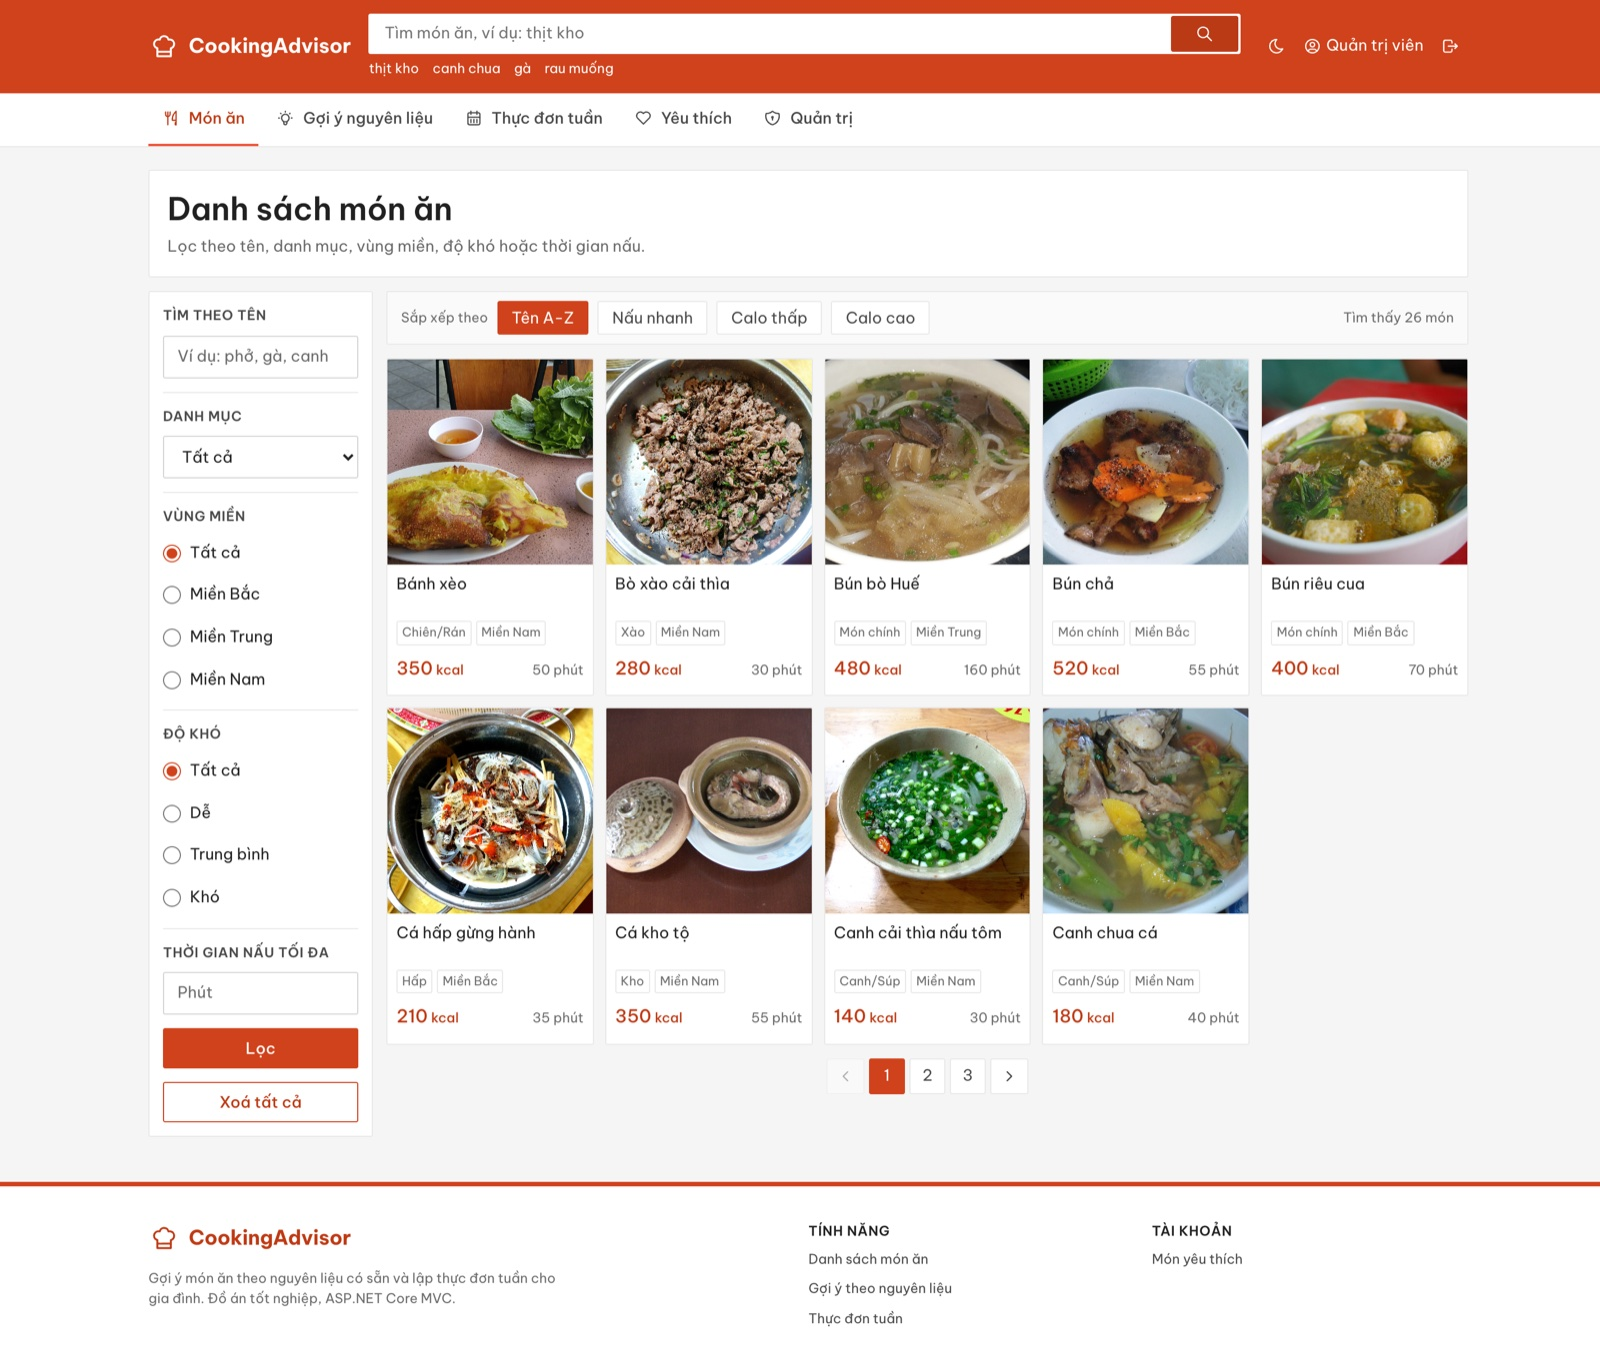
\includegraphics[width=0.65\textwidth]{h4-02-danh-sach-mon.jpg}
\caption{Trang danh sách món ăn với bộ lọc bên trái và lưới kết quả}
\label{fig:h4-02}
\end{figure}

Màn hình danh sách gồm ô tìm kiếm theo tên (chức năng A3), nhóm bộ lọc bên trái
theo danh mục, vùng miền, độ khó và thời gian nấu tối đa (A4), hộp chọn sắp xếp
với bốn phương án tên A-Z, nấu nhanh, calo thấp, calo cao (A5), và lưới thẻ món
phân trang 9 món mỗi trang; các liên kết phân trang giữ nguyên trạng thái lọc và
sắp xếp hiện tại. Nút thêm yêu thích trên từng thẻ chỉ hiện với người dùng đã
đăng nhập. Bấm vào một thẻ mở trang chi tiết, nơi hiển thị đầy đủ thông số, danh
sách nguyên liệu kèm định lượng và các bước nấu.

\subsection{Tìm kiếm, lọc và sắp xếp}

Khi lọc theo vùng miền Nam, độ khó Dễ và sắp xếp theo năng lượng tăng dần, số
món giảm từ 26 xuống còn tập con thỏa mãn cả hai điều kiện, đồng thời thứ tự
hiển thị tuân theo tiêu chí đã chọn; các liên kết sắp xếp và phân trang đều giữ
nguyên trạng thái lọc hiện tại. Tính đúng đắn của từng phương án sắp xếp được
kiểm chứng bằng các ca kiểm thử TC-24 tới TC-29 ở mục~\ref{sec:kiem-thu}.

\subsection{Gợi ý theo nguyên liệu}

Trang gợi ý liệt kê toàn bộ nguyên liệu dưới dạng bảng hộp kiểm sắp theo tên.
Khi người dùng chưa chọn nguyên liệu nào, trang giữ trạng thái ban đầu kèm hướng
dẫn sử dụng thay vì trả về danh sách rỗng.

\begin{figure}[H]
\centering
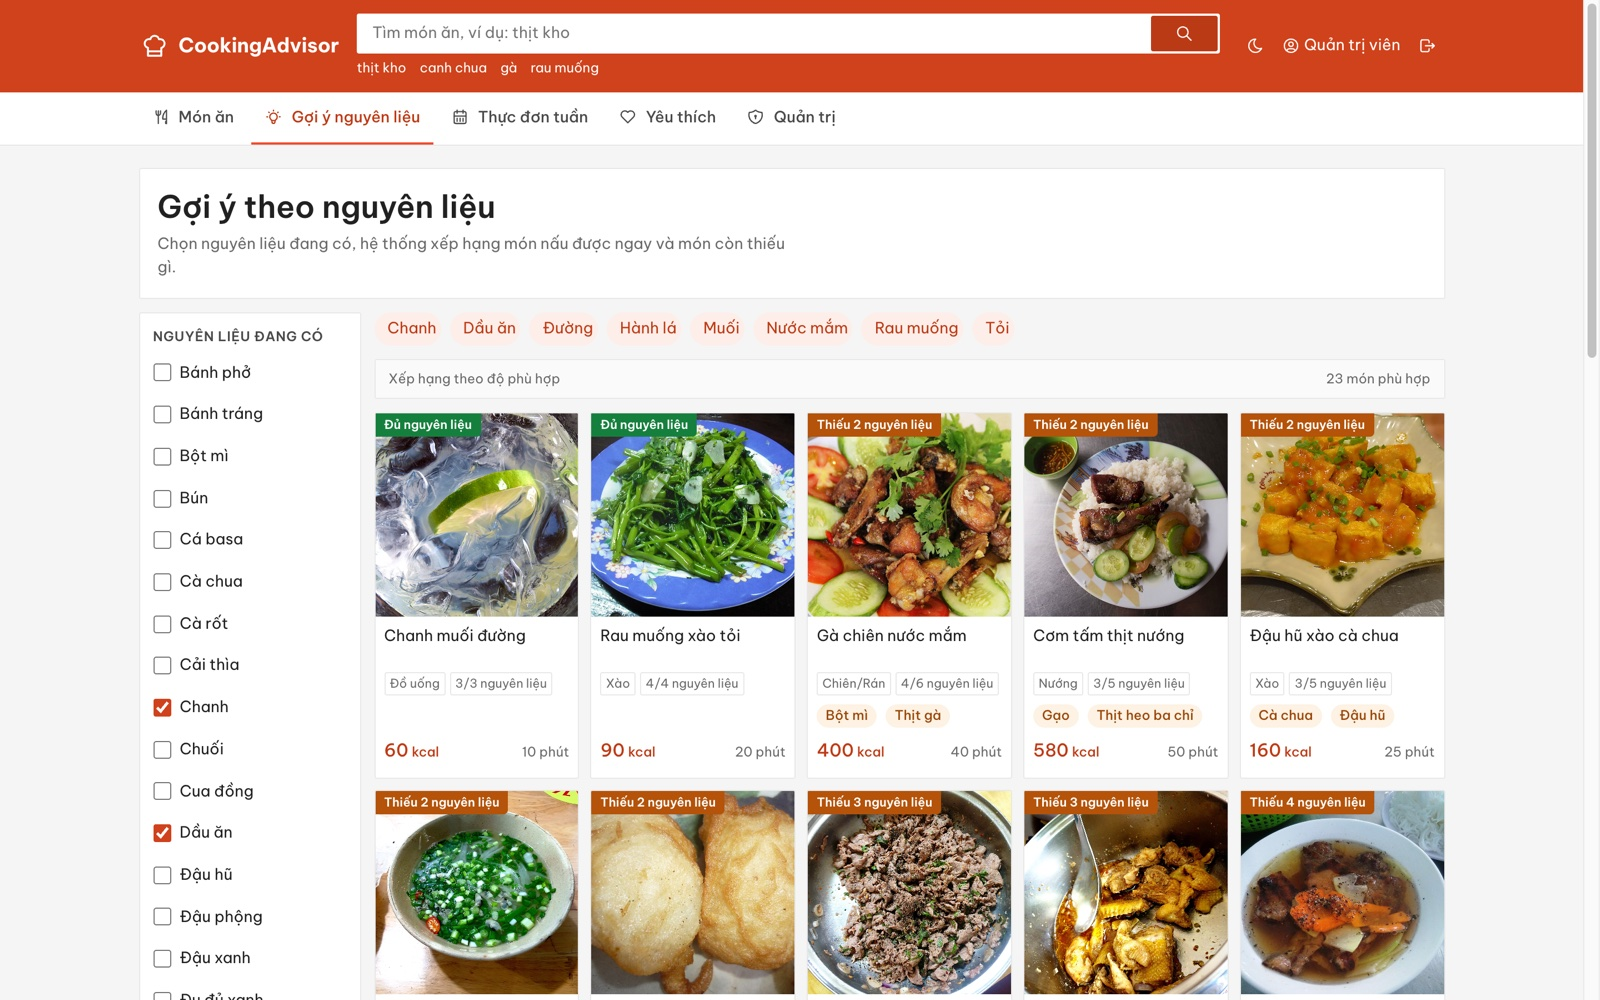
\includegraphics[width=0.67\textwidth]{h4-06-goi-y-ket-qua.jpg}
\caption{Kết quả gợi ý với 8 nguyên liệu đầu vào}
\label{fig:h4-06}
\end{figure}

Với đầu vào gồm 8 nguyên liệu (chanh, dầu ăn, đường, hành lá, muối, nước mắm, rau
muống, tỏi), hệ thống trả về \textbf{24 món phù hợp}, trong đó \textbf{2 món nấu
được ngay} và 22 món còn thiếu nguyên liệu. Hai món nấu được ngay được xếp lên
đầu danh sách và mang nhãn màu xanh ``Đủ nguyên liệu''; các món còn lại mang nhãn
màu hổ phách ghi rõ số nguyên liệu còn thiếu, kèm danh sách tên nguyên liệu đó
ngay dưới tên món. Nhãn ``Đủ nguyên liệu'' được gắn cho món có độ phủ bằng 1,
tương ứng $M = \emptyset$; thứ tự các thẻ kết quả phản ánh trực tiếp bốn tiêu
chí xếp hạng đã thiết kế ở mục~\ref{sec:thuat-toan-goi-y}.

\subsection{Thực đơn tuần}

Trang thực đơn gồm biểu mẫu sinh thực đơn (nhập tên, chọn tuần bắt đầu và vùng
miền nếu muốn, ứng với chức năng B1) và danh sách các thực đơn đã lưu của riêng
người dùng đang đăng nhập (B4).

\begin{figure}[H]
\centering
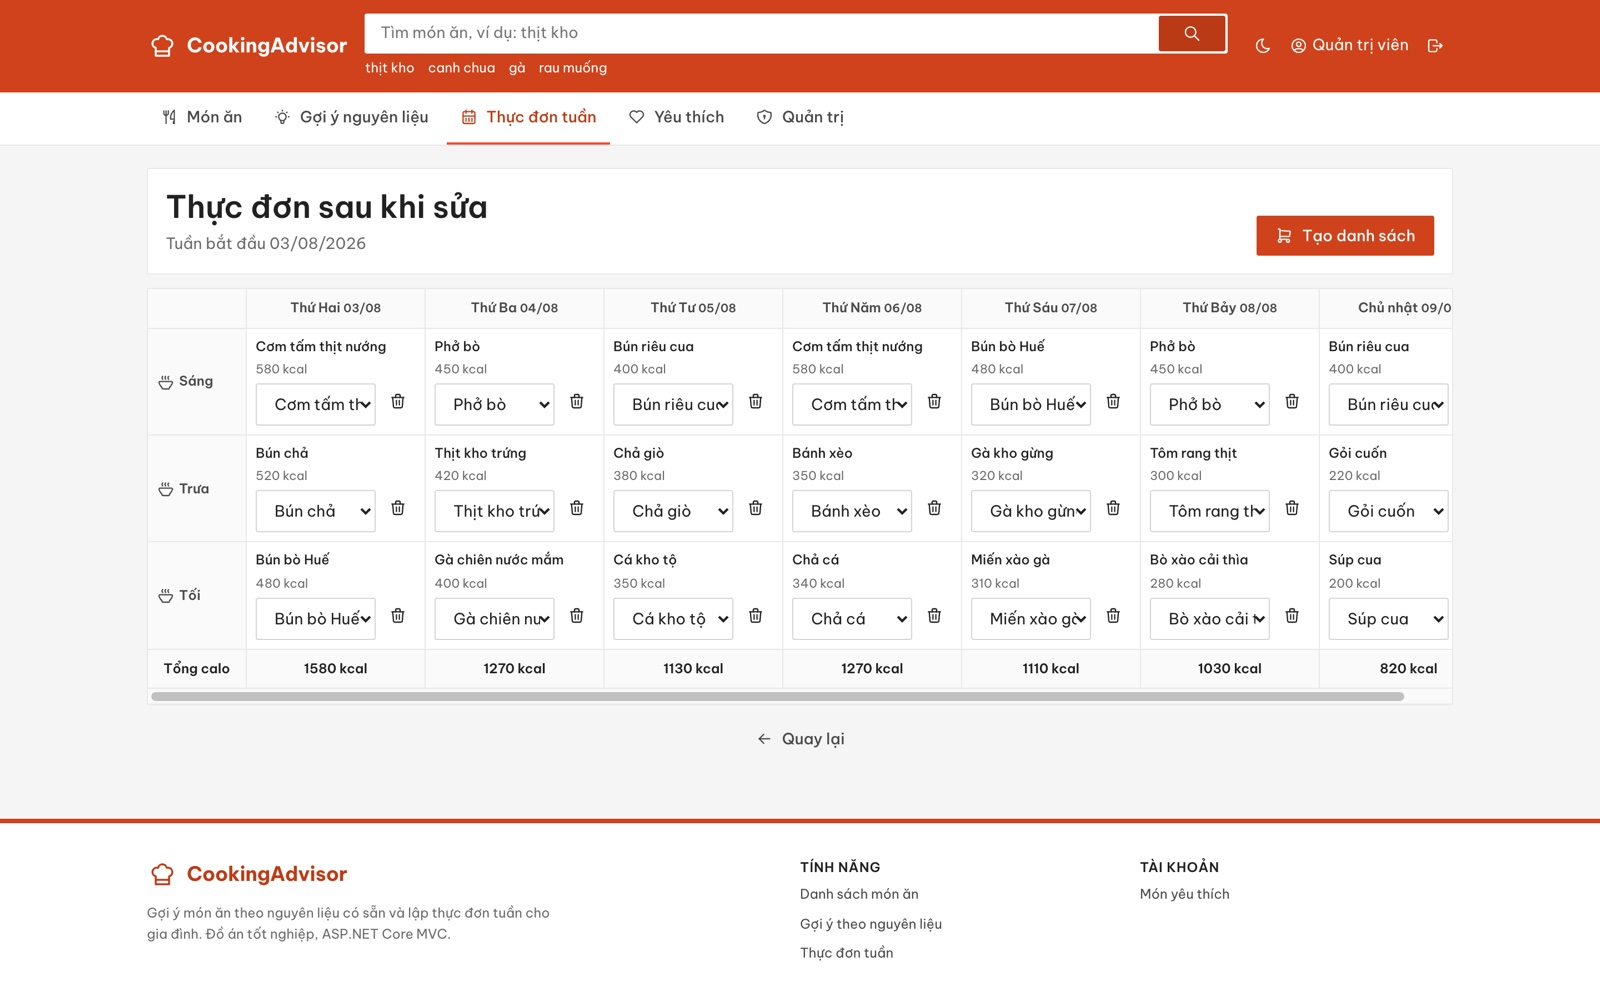
\includegraphics[width=0.70\textwidth]{h4-08-thuc-don-tuan.jpg}
\caption{Lịch thực đơn 7 ngày $\times$ 3 bữa}
\label{fig:h4-08}
\end{figure}

Lưới thực đơn hiển thị đủ 21 suất ăn, mỗi ô ứng với một bản ghi
\code{MenuPlanItem} gồm tên món, năng lượng theo khẩu phần, một hộp chọn để đổi
sang món khác và một nút xóa (chức năng B3); cột của ngày vẫn được giữ lại kể cả
khi cả ba bữa đều trống. Dòng cuối cùng hiển thị tổng năng lượng theo từng ngày,
lần lượt là 1580, 1270, 1130, 1270, 1110, 1030 và 820 kcal, được tính lại sau
mỗi lần chỉnh sửa. Nút ``Tạo danh sách đi chợ'' chuyển sang chức năng B5 với mã
thực đơn hiện tại.

\subsection{Danh sách đi chợ}

\begin{figure}[H]
\centering
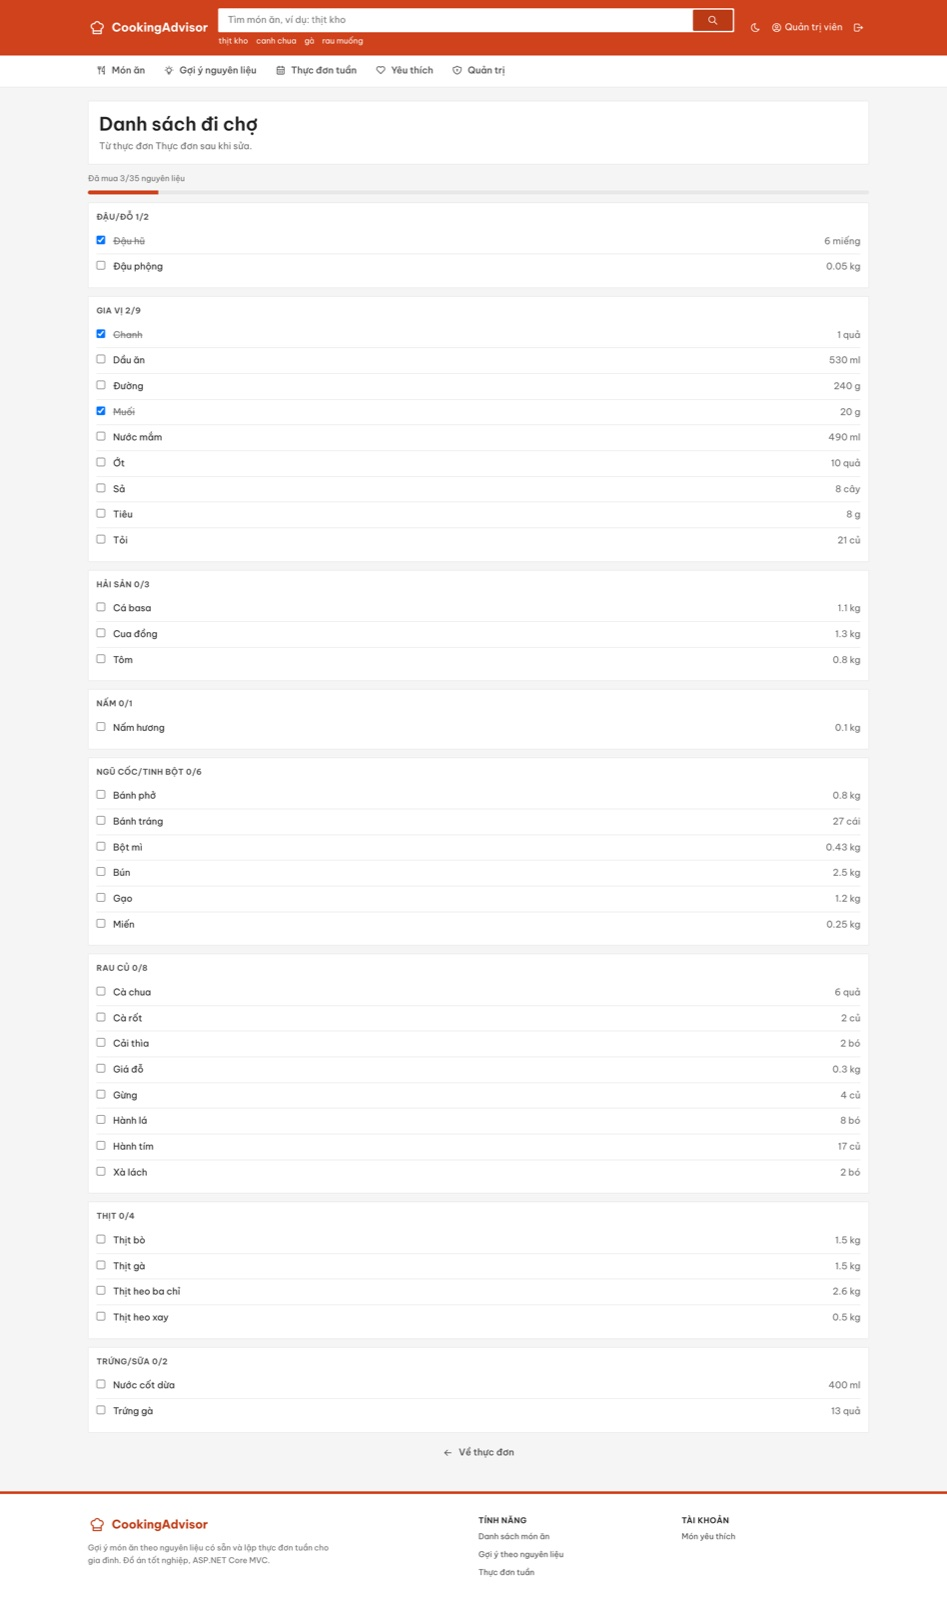
\includegraphics[height=0.44\textheight]{h4-09-di-cho.jpg}
\caption{Danh sách đi chợ sinh từ thực đơn ở Hình~\ref{fig:h4-08}}
\label{fig:h4-09}
\end{figure}

Từ thực đơn 21 suất ăn, hệ thống sinh ra danh sách gồm \textbf{35 dòng nguyên
liệu} được gộp theo \textbf{8 nhóm}: Đậu/Đỗ, Gia vị, Hải sản, Nấm, Ngũ cốc/Tinh
bột, Rau củ, Thịt và Trứng/Sữa; tiêu đề nhóm lấy theo cột \code{Group} của bảng
\code{Ingredients}. Mỗi dòng hiển thị tên nguyên liệu, tổng khối lượng đã cộng
dồn và đơn vị, kèm hộp kiểm ``đã mua'' đảo trạng thái \code{IsPurchased}; thanh
tiến độ ở đầu trang cập nhật theo số dòng đã đánh dấu. Nút tạo lại danh sách ghi
đè danh sách cũ để phản ánh thực đơn vừa chỉnh sửa.

\subsection{Tài khoản và phân quyền}

Biểu mẫu đăng nhập xác thực bằng thư điện tử và mật khẩu; khi thông tin sai, hệ
thống báo lỗi chung mà không tiết lộ sai ở trường nào.

Cơ chế kiểm tra hợp lệ của biểu mẫu đăng ký hoạt động đồng thời trên ba trường:
sai định dạng email, mật khẩu ngắn hơn 8 ký tự và mật khẩu xác nhận không khớp.
Thông báo lỗi hiển thị bằng tiếng Việt ngay dưới ô nhập tương ứng, viền ô nhập
chuyển sang màu đỏ.

Yêu cầu phi chức năng N2 cũng được kiểm chứng trực tiếp trên hệ thống đang chạy:
một tài khoản vừa đăng ký với vai trò \code{User} khi truy cập đường dẫn
\code{/Admin/Recipes} bị chuyển hướng sang trang thông báo không đủ quyền, kèm
tham số \code{ReturnUrl} ghi nhận trang đã bị chặn.

Sau khi đăng nhập, người dùng còn sử dụng được trang danh sách món yêu thích
(chức năng B7): thêm hoặc bỏ yêu thích ngay trên thẻ món và xem lại toàn bộ món
đã đánh dấu; các món này được thuật toán sinh thực đơn ưu tiên chọn.

\subsection{Khu vực quản trị}

Khu vực quản trị gồm bảng điều khiển với thẻ số liệu tổng quan (chức năng C1),
các bảng quản lý món ăn, nguyên liệu và danh mục với nút thêm, sửa, xóa (C2 tới
C4). Biểu mẫu món ăn cho phép nhập thông số món rồi gán từng nguyên liệu kèm
khối lượng và đơn vị ngay trên cùng một trang. Thao tác xóa nguyên liệu đang
được tham chiếu hoặc danh mục còn món sử dụng bị chặn kèm thông báo giải thích,
đúng như thiết kế hành vi xóa ở mục~\ref{sec:hanh-vi-xoa}.

\subsection{Giao diện đáp ứng và chế độ tối}

Trên màn hình hẹp, bố cục các trang tự sắp xếp lại thành một cột và nhóm bộ lọc
của trang danh sách chuyển thành ngăn kéo trượt mở từ cạnh màn hình. Hệ thống
cũng hỗ trợ chế độ tối: toàn bộ cặp màu chữ và
nền được định nghĩa lại qua biến CSS, và các trang hiển thị trạng thái rỗng có
hướng dẫn thay vì bảng trống khi chưa có dữ liệu.

\section{Kịch bản demo}
\label{sec:demo}

Luồng sử dụng xuyên suốt ba chức năng lõi diễn ra như sau. Người dùng mở mục
``Gợi ý nguyên liệu'', tick 8 nguyên liệu đang có rồi bấm ``Gợi ý món'' và nhận
về 24 món xếp hạng với 2 món nấu được ngay ở đầu danh sách
(Hình~\ref{fig:h4-06}); mở chi tiết vài món và bấm ``Thêm yêu thích'' để các món
đó được ưu tiên khi sinh thực đơn. Sang mục ``Thực đơn tuần'', nhập tên, chọn
tuần bắt đầu rồi bấm ``Tạo thực đơn'', hệ thống sinh đủ 21 suất ăn trong một
thao tác (Hình~\ref{fig:h4-08}); ô nào chưa vừa ý thì chọn món khác ngay trong ô
đó và tổng năng lượng của ngày được tính lại. Cuối cùng bấm ``Tạo danh sách'' để
gộp nguyên liệu của 21 suất thành 35 dòng theo 8 nhóm (Hình~\ref{fig:h4-09});
khi đi chợ, mua xong nguyên liệu nào thì tick vào ô tương ứng, dòng đó bị gạch
ngang và thanh tiến độ tăng lên.

\section{Kết quả kiểm thử}
\label{sec:kiem-thu}

\subsection{Phương pháp kiểm thử}

Kiểm thử được thực hiện ở mức \textbf{kiểm thử đơn vị} bằng thư viện xUnit, tập
trung vào ba lớp dịch vụ chứa thuật toán lõi cùng chức năng sắp xếp danh sách
món. Cơ sở dữ liệu được thay bằng nhà cung cấp \textbf{EF Core In-Memory}, nhờ đó
các ca kiểm thử chạy độc lập, không phụ thuộc vào SQL Server và không để lại dữ
liệu thừa. Mỗi ca kiểm thử tạo một cơ sở dữ liệu riêng mang tên ngẫu nhiên, bảo
đảm các ca không ảnh hưởng lẫn nhau.

Việc kiểm thử được ở mức này là kết quả trực tiếp của quyết định kiến trúc đã nêu
ở mục~\ref{sec:kien-truc}: vì logic nghiệp vụ nằm ở tầng Service chứ không nằm
trong Controller, nên có thể khởi tạo và kiểm thử trực tiếp mà không cần hạ tầng
web.

Cần lưu ý một giới hạn của cách tiếp cận này: nhà cung cấp In-Memory
\textbf{không thực thi} ràng buộc duy nhất, khóa ngoại hay quy tắc so sánh chuỗi
của SQL Server. Vì vậy các ca kiểm thử ở đây kiểm chứng logic của thuật toán, còn
các hành vi phụ thuộc vào cơ sở dữ liệu thật (tranh chấp ghi đồng thời, vi phạm
khóa ngoại, thứ tự sắp xếp theo bảng mã tiếng Việt) nằm ngoài vùng phủ và được
kiểm tra thủ công trên môi trường chạy thật.

\subsection{Kết quả chạy kiểm thử}

Bộ kiểm thử gồm \textbf{29 ca}, chia theo bốn nhóm ứng với ba thuật toán lõi và
chức năng tìm kiếm, sắp xếp. Danh sách đầy đủ từ TC-01 tới TC-29 kèm mục tiêu
kiểm chứng của từng ca được liệt kê ở Phụ lục F. Lệnh
\code{dotnet test src/CookingAdvisor.sln} cho kết quả:

\begin{codeblock}
Test run for .../CookingAdvisor.Tests.dll
    (.NETCoreApp,Version=v10.0)
A total of 1 test files matched the specified pattern.

Passed!  - Failed: 0, Passed: 29, Skipped: 0, Total: 29,
Duration: 337 ms - CookingAdvisor.Tests.dll (net10.0)
\end{codeblock}

\begin{table}[H]
\centering
\caption{Tổng hợp kết quả kiểm thử theo nhóm}
\label{tab:tong-hop-kiem-thu}
\begin{tabularx}{\textwidth}{|Y|P{2.0cm}|P{2.0cm}|P{2.4cm}|}
\hline
\bfseries Nhóm & \bfseries Số ca & \bfseries Đạt & \bfseries Không đạt \\ \hline
\code{SuggestionService} & 6 & 6 & 0 \\ \hline
\code{MenuPlannerService} & 9 & 9 & 0 \\ \hline
\code{ShoppingListService} & 8 & 8 & 0 \\ \hline
\code{RecipeService} & 6 & 6 & 0 \\ \hline
\bfseries Tổng & \bfseries 29 & \bfseries 29 & \bfseries 0 \\ \hline
\end{tabularx}
\end{table}

\subsection{Khiếm khuyết phát hiện qua kiểm thử}
\label{sec:khiem-khuyet}

Quá trình kiểm thử đã phát hiện hai khiếm khuyết mà quan sát bằng mắt thường khó
nhận ra. Đây là kết quả có giá trị nhất của phần kiểm thử.

\noindent\textbf{Khiếm khuyết 1: suy thoái tính đa dạng của thực đơn.}

\textit{Hiện tượng.} Khi thư viện món không đủ lấp 21 suất mà không lặp, thuật
toán chọn lại đúng một món cho hầu hết các suất còn trống.

\textit{Đo lường.} Trên bộ dữ liệu thử, một món xuất hiện 12 lần trong khi nhiều
món khác dùng được lại không được chọn lần nào. Con số này là kết quả đo tại thời
điểm phát hiện khiếm khuyết, trước khi vá.

\textit{Nguyên nhân.} Như đã phân tích ở mục~\ref{sec:thuat-toan-thuc-don}, trong
nhánh phải lặp, tiêu chí quyết định lùi về khoảng cách năng lượng. Do trạng thái
năng lượng tích lũy lặp lại theo chu kỳ, cùng một món luôn cho khoảng cách nhỏ
nhất.

\textit{Khắc phục.} Bổ sung tiêu chí ưu tiên món có số lần đã dùng ít nhất, đặt
trước tiêu chí năng lượng và chỉ áp dụng trong nhánh lặp.

\textit{Kết quả sau khắc phục.} Thực đơn sinh ra đạt \textbf{17 món khác nhau
trên 21 suất}. Hai ca kiểm thử hồi quy TC-10 và TC-11 được bổ sung để ngăn khiếm
khuyết tái diễn.

\noindent\textbf{Khiếm khuyết 2: thứ tự không xác định khi phân trang.}

\textit{Hiện tượng.} Khi sắp xếp theo năng lượng, các món có cùng giá trị năng
lượng không có thứ tự tất định giữa hai lần truy vấn, dẫn tới nguy cơ một món
xuất hiện ở cả trang trước và trang sau.

\textit{Nguyên nhân.} Câu lệnh sắp xếp chỉ có một khóa duy nhất. Với các bản ghi
có khóa bằng nhau, hệ quản trị cơ sở dữ liệu được tự do trả về theo thứ tự bất
kỳ.

\textit{Khắc phục.} Bổ sung khóa sắp xếp phụ là tên món cho mọi phương án sắp
xếp.

\textit{Kiểm chứng.} Ca kiểm thử TC-28 dựng 12 món có cùng giá trị năng lượng,
\textbf{nạp theo thứ tự tên giảm dần} để loại trừ khả năng kết quả đúng chỉ nhờ
trùng với thứ tự chèn dữ liệu, sau đó yêu cầu hai trang liên tiếp và kiểm tra
không có món nào lặp lại. Ca kiểm thử này đã được xác nhận là \textbf{có hiệu
lực}: khi tạm gỡ khóa sắp xếp phụ khỏi mã nguồn, ca kiểm thử chuyển sang trạng
thái không đạt; khi khôi phục, ca kiểm thử đạt trở lại.

\subsection{Kiểm thử giao diện}
\label{sec:kiem-thu-giao-dien}

Ngoài kiểm thử tự động ở mức đơn vị, giao diện được kiểm tra thủ công trên trình
duyệt theo các tiêu chí phi chức năng đã nêu ở
mục~\ref{sec:yeu-cau-phi-chuc-nang}.

\begin{table}[H]
\centering
\caption{Kết quả kiểm tra giao diện theo tiêu chí phi chức năng}
\label{tab:kiem-thu-giao-dien}
\begin{tabularx}{\textwidth}{|P{3.4cm}|Y|Y|}
\hline
\bfseries Tiêu chí & \bfseries Cách kiểm tra & \bfseries Kết quả \\ \hline
N4, không cuộn ngang & Đo \code{scrollWidth} so với \code{clientWidth} ở 375 px
  trên các trang chính & Đạt, không trang nào cuộn ngang \\ \hline
N5, tương phản WCAG AA & Đo tỉ lệ tương phản của các cặp màu chữ và nền
  trên trang thật & Đạt, cặp thấp nhất 4,69:1 so với ngưỡng 4,5:1 \\ \hline
Chế độ tối & Chuyển chế độ và đo lại toàn bộ cặp màu & Đạt ở cả hai chế độ \\ \hline
Điều hướng bàn phím & Kiểm tra bộ lọc dạng ngăn kéo: mở, giữ tiêu điểm,
  đóng bằng phím Esc & Đạt \\ \hline
Nhật ký lỗi trình duyệt & Theo dõi bảng điều khiển của trình duyệt khi duyệt các
  trang & Không có lỗi \\ \hline
\end{tabularx}
\end{table}

\section{Đánh giá}
\label{sec:danh-gia}

\subsection{Kết quả đạt được}
\label{sec:ket-qua-dat-duoc}

Đối chiếu với sáu mục tiêu đề ra ở phần Mở đầu:

\begin{table}[H]
\centering
\caption{Đối chiếu kết quả đạt được với mục tiêu đề ra}
\label{tab:doi-chieu-muc-tieu}
\begin{tabularx}{\textwidth}{|P{5.6cm}|Y|}
\hline
\bfseries Mục tiêu & \bfseries Kết quả \\ \hline
1. Quản lý kho dữ liệu món ăn & Đạt, 26 món với đầy đủ thuộc tính và định lượng
  nguyên liệu \\ \hline
2. Thuật toán gợi ý theo nguyên liệu & Đạt, 6 ca kiểm thử đều đạt \\ \hline
3. Thuật toán sinh thực đơn tuần & Đạt, 9 ca kiểm thử đều đạt \\ \hline
4. Sinh danh sách đi chợ & Đạt, 8 ca kiểm thử đều đạt \\ \hline
5. Xác thực và phân quyền & Đạt, kiểm chứng trên hệ thống đang chạy \\ \hline
6. Kiểm chứng bằng kiểm thử tự động & Đạt, 29 ca kiểm thử, phát hiện 2
  khiếm khuyết thực tế \\ \hline
\end{tabularx}
\end{table}

\subsection{Hạn chế}
\label{sec:han-che}

Hệ thống còn các hạn chế sau, được nêu đầy đủ để làm cơ sở cho phần Hướng phát
triển ở Chương~\ref{ch:ket-luan}:

\textbf{Một là gợi ý chưa xét định lượng:} thuật toán hiện chỉ xét việc có hay
không có một nguyên liệu, chưa xét người dùng có đủ khối lượng hay không, nên
một người có 50 gam thịt vẫn được gợi ý món cần 500 gam. \textbf{Hai là chưa cá
nhân hóa:} kết quả gợi ý chỉ phụ thuộc tập nguyên liệu đầu vào, giống nhau với
mọi người dùng, lịch sử nấu ăn chưa được khai thác. \textbf{Ba là dinh dưỡng ở
mức thô:} mới dừng ở năng lượng theo khẩu phần, chưa bóc tách đạm, béo, tinh bột
hay vi chất. \textbf{Bốn là} ảnh minh họa nhập bằng đường dẫn, chưa có chức năng
tải ảnh lên. \textbf{Năm là} chưa có đổi mật khẩu, quên mật khẩu và xác thực
email. \textbf{Sáu là} khu quản trị chưa phân trang và chưa có tìm kiếm, với quy
mô dữ liệu mẫu hiện tại thì chưa gây trở ngại nhưng sẽ là hạn chế khi số món
tăng lên. \textbf{Bảy là} thuật toán lập thực đơn theo hướng tham lam nên không
bảo đảm nghiệm tối ưu toàn cục về cân đối năng lượng. \textbf{Tám là} chưa có
kiểm thử tích hợp và kiểm thử giao diện tự động, phần giao diện mới được kiểm
tra thủ công.

% ============================================================
%  CHUONG 5. KET LUAN VA HUONG PHAT TRIEN
% ============================================================
\chapter{Kết luận và hướng phát triển}
\label{ch:ket-luan}

\section{Kết luận}

Đồ án đã hoàn thành việc xây dựng \textbf{CookingAdvisor}, một ứng dụng web hỗ
trợ người nấu ăn trong gia đình ở ba khâu: tìm món từ nguyên liệu sẵn có, lập
thực đơn cho cả tuần và tổng hợp danh sách đi chợ.

\subsection{Kết quả đạt được}

\textbf{Về mặt chức năng,} hệ thống cung cấp 20 chức năng phân thành ba nhóm theo
mức quyền truy cập, chạy hoàn chỉnh đầu-cuối trên cơ sở dữ liệu mẫu gồm 26 món ăn
Việt Nam, 40 nguyên liệu và 10 danh mục. Toàn bộ sáu mục tiêu đặt ra ở phần Mở
đầu đều đã đạt, với kết quả kiểm chứng cụ thể trình bày ở
mục~\ref{sec:ket-qua-dat-duoc}.

\textbf{Về mặt thuật toán,} ba thuật toán lõi đã được thiết kế, cài đặt và kiểm
chứng:

\begin{itemize}
  \item \textit{Thuật toán gợi ý theo nguyên liệu} sử dụng độ phủ tập hợp kết hợp
        xếp hạng bốn tiêu chí. Đóng góp đáng chú ý ở đây là lập luận chọn độ phủ
        thay cho hệ số Jaccard: do Jaccard là độ đo đối xứng nên nó phạt cả phần
        nguyên liệu dư của người dùng, dẫn tới việc một món nấu được ngay có thể
        bị xếp hạng rất thấp.
  \item \textit{Thuật toán sinh thực đơn tuần} theo hướng tham lam có ràng buộc,
        với thứ tự nới lỏng ràng buộc được quy định rõ ràng và ràng buộc vùng
        miền được giữ cứng.
  \item \textit{Thuật toán sinh danh sách đi chợ} gộp nhóm theo khóa ghép (nguyên
        liệu, đơn vị), bảo đảm không cộng dồn nhầm hai giá trị khác đơn vị.
\end{itemize}

\textbf{Về mặt kiểm chứng,} bộ 29 ca kiểm thử đơn vị đã phát hiện được hai khiếm
khuyết mà việc quan sát bằng mắt thường khó nhận ra:

\begin{enumerate}[label=\arabic*.]
  \item \textit{Suy thoái tính đa dạng của thực đơn.} Khi thư viện món không đủ
        lớn, tiêu chí phụ theo năng lượng khiến thuật toán chọn lại đúng một món
        cho hầu hết các suất còn trống, đo được là một món chiếm 12 suất. Sau khi
        bổ sung tiêu chí rải đều theo số lần đã dùng, thực đơn đạt 17 món khác
        nhau trên 21 suất.
  \item \textit{Thứ tự không xác định khi phân trang.} Việc sắp xếp chỉ theo một
        khóa duy nhất khiến các bản ghi có giá trị bằng nhau không có thứ tự ổn
        định, dẫn tới nguy cơ một món xuất hiện ở hai trang. Đã khắc phục bằng
        khóa sắp xếp phụ theo tên món.
\end{enumerate}

Việc phát hiện được hai khiếm khuyết này là minh chứng cho giá trị thực tế của
kiểm thử tự động, đồng thời cho thấy quyết định kiến trúc tách tầng Service khỏi
tầng Controller (mục~\ref{sec:kien-truc}) đã phát huy tác dụng: nếu logic nằm
trong Controller, việc viết các ca kiểm thử này sẽ khó khăn hơn nhiều.

\textbf{Về mặt giao diện,} hệ thống hiển thị đúng trên dải màn hình từ 375 px tới
1440 px, không xuất hiện cuộn ngang, hỗ trợ chế độ tối và đạt chuẩn tương phản
WCAG 2.1 mức AA với cặp màu thấp nhất đo được là 4,69:1.

\subsection{Đóng góp của đồ án}

So với các ứng dụng đã khảo sát ở mục~\ref{sec:khao-sat}, đồ án có ba điểm khác
biệt.

\textbf{Thứ nhất, tích hợp trọn vẹn ba chức năng trong một luồng công việc liền
mạch.} Các sản phẩm khảo sát thường mạnh ở một khâu và thiếu ở khâu khác. Mealime
lập được thực đơn nhưng không hỗ trợ truy vấn ngược từ nguyên liệu. Paprika quản
lý công thức và danh sách đi chợ tốt nhưng không tự động hóa việc lập thực đơn.
Các trang trong nước chủ yếu dừng ở việc cung cấp nội dung.

\textbf{Thứ hai, dữ liệu món ăn Việt Nam được chuẩn hóa về định lượng.} Bảng
trung gian giữa món ăn và nguyên liệu mang thêm thuộc tính khối lượng và đơn vị.
Đây là điều kiện tiên quyết để danh sách đi chợ có thể cộng dồn chính xác, điều
mà các nền tảng có nội dung do cộng đồng đóng góp khó bảo đảm.

\textbf{Thứ ba, thuật toán minh bạch và kiểm chứng được.} Toàn bộ tiêu chí xếp
hạng và thứ tự nới lỏng ràng buộc đều được phát biểu tường minh, có mã giả, có
lưu đồ và có ca kiểm thử tương ứng.

\subsection{Hạn chế}

Đồ án còn tám hạn chế đã nêu chi tiết ở mục~\ref{sec:han-che}. Trong đó, ba hạn
chế có ảnh hưởng lớn nhất tới trải nghiệm người dùng là:

\begin{itemize}
  \item Thuật toán gợi ý mới xét việc \textbf{có hay không có} một nguyên liệu,
        chưa xét người dùng có \textbf{đủ khối lượng} hay không.
  \item Kết quả gợi ý \textbf{giống nhau với mọi người dùng}, chưa khai thác lịch
        sử nấu ăn để cá nhân hóa.
  \item Thông tin dinh dưỡng mới dừng ở \textbf{năng lượng theo khẩu phần}, chưa
        bóc tách các thành phần dinh dưỡng chi tiết.
\end{itemize}

\section{Hướng phát triển}

\subsection{Hoàn thiện các thuật toán hiện có}

\textbf{Gợi ý có xét định lượng.} Mở rộng mô hình dữ liệu để người dùng khai báo
được khối lượng nguyên liệu đang có, không chỉ khai báo có hay không. Khi đó điều
kiện ``nấu được ngay'' trở thành: với mọi nguyên liệu $i$ của món, khối lượng
người dùng có phải lớn hơn hoặc bằng khối lượng công thức yêu cầu. Thay đổi này
cũng cho phép danh sách đi chợ \textbf{trừ đi phần đã có}, chỉ liệt kê phần còn
thiếu.

\textbf{Lập thực đơn theo hướng tối ưu.} Thay chiến lược tham lam bằng một thuật
toán tìm kiếm cục bộ hoặc quy hoạch ràng buộc, để tổng năng lượng theo ngày bám
sát mục tiêu hơn. Có thể bổ sung các ràng buộc mới như cân đối nhóm thực phẩm
trong tuần hoặc tránh lặp cùng một nguyên liệu chính trong hai ngày liên tiếp.

\textbf{Cá nhân hóa kết quả gợi ý.} Khi hệ thống đã tích lũy đủ dữ liệu về lịch
sử nấu ăn và món yêu thích, có thể áp dụng kỹ thuật lọc cộng tác để bổ sung một
tiêu chí xếp hạng dựa trên mức độ phù hợp với khẩu vị của từng người dùng. Cần
lưu ý đây là hướng chỉ khả thi khi đã có người dùng thực, do các phương pháp này
gặp vấn đề khởi đầu nguội trên hệ thống mới.

\subsection{Mở rộng chức năng}

\begin{table}[H]
\centering
\caption{Các hướng mở rộng chức năng}
\label{tab:mo-rong}
\begin{tabularx}{\textwidth}{p{4.2cm} Y}
\toprule
\bfseries Hướng mở rộng & \bfseries Nội dung \\
\midrule
Dinh dưỡng chi tiết & Bổ sung đạm, béo, tinh bột, chất xơ; cảnh báo theo chế độ
  ăn hoặc bệnh lý \\
\rowhl Quản lý tài khoản & Đổi mật khẩu, quên mật khẩu, xác thực email, trang hồ
  sơ cá nhân \\
Tải ảnh lên & Thay việc nhập đường dẫn ảnh bằng chức năng tải tệp và tự tạo ảnh
  thu nhỏ \\
\rowhl Cộng đồng & Cho phép người dùng đóng góp công thức, đánh giá và bình
  luận \\
Chia sẻ thực đơn & Xuất thực đơn tuần ra tệp hoặc chia sẻ qua đường dẫn công
  khai \\
\rowhl In danh sách đi chợ & Xuất bản in hoặc tệp PDF để mang theo khi đi chợ \\
\bottomrule
\end{tabularx}
\end{table}

\subsection{Cải thiện kỹ thuật}

\textbf{Phân trang và tìm kiếm cho khu quản trị.} Hiện các danh sách trong khu
quản trị hiển thị toàn bộ bản ghi. Với quy mô dữ liệu mẫu thì chưa gây trở ngại,
nhưng sẽ trở thành hạn chế khi số món tăng lên.

\textbf{Bổ sung kiểm thử tích hợp và kiểm thử giao diện tự động.} Hiện phần giao
diện mới được kiểm tra thủ công. Có thể bổ sung kiểm thử tích hợp cho các luồng
Controller và kiểm thử giao diện tự động cho các kịch bản chính. Việc này cũng
giúp phủ được nhóm hành vi mà nhà cung cấp EF Core In-Memory không mô phỏng được,
như đã nêu ở mục~\ref{sec:kiem-thu}.

\textbf{Ứng dụng di động.} Bối cảnh sử dụng thực tế của chức năng danh sách đi
chợ là khi người dùng đang ở chợ hoặc siêu thị. Một ứng dụng di động có khả năng
hoạt động ngoại tuyến sẽ phù hợp hơn giao diện web.

% ============================================================
%  DANH MUC TAI LIEU THAM KHAO
%  Dinh dang IEEE, xep theo thu tu tu dien. GIU NGUYEN thu tu
%  danh so nay, moi trich dan trong than bai deu bam theo.
% ============================================================
\unnumberedchapter{DANH MỤC TÀI LIỆU THAM KHẢO}

Danh mục xếp theo thứ tự từ điển và trình bày theo định dạng IEEE, thống nhất cho
toàn bộ báo cáo.

% Nhan [n] can nam sat le trai; dinh nghia ngoai moi truong list de tranh
% ky tu # trong tham so cua \begin{list}.
\newcommand{\tltklabel}[1]{#1\hfill}

\begin{list}{}{%
  \setlength{\labelwidth}{2.2em}
  \setlength{\leftmargin}{2.6em}
  \setlength{\labelsep}{0.4em}
  \setlength{\itemsep}{4pt}
  \setlength{\parsep}{0pt}
  \let\makelabel\tltklabel
}

\item[{[1]}] Apple App Store, ``Cookpad Recipes''. [Online]. Địa chỉ:
\url{https://apps.apple.com/us/app/cookpad-recipes/id340368403}. [Truy cập ngày
25/07/2026].

\item[{[2]}] Apple App Store, ``Mealime Meal Plans \& Recipes''. [Online]. Địa
chỉ: \url{https://apps.apple.com/us/app/mealime-meal-plans-recipes/id1079999103}.
[Truy cập ngày 25/07/2026].

\item[{[3]}] Apple App Store, ``Paprika Recipe Manager 3''. [Online]. Địa chỉ:
\url{https://apps.apple.com/us/app/paprika-recipe-manager-3/id1303222628}. [Truy
cập ngày 25/07/2026].

\item[{[4]}] CafeF, ``Thị trường quá khốc liệt, Cooky, startup đi chợ online của
Founder ShopeeFood rời thị trường Hà Nội, chỉ còn hoạt động tại TPHCM''.
[Online]. Địa chỉ:
\url{https://cafef.vn/thi-truong-qua-khoc-liet-cooky-startup-di-cho-online-cua-founder-shopeefood-roi-thi-truong-ha-noi-chi-con-hoat-dong-tai-tphcm-188231205162148255.chn}.
[Truy cập ngày 25/07/2026].

\item[{[5]}] Cookpad, ``Cookpad Việt Nam''. [Online]. Địa chỉ:
\url{https://cookpad.com/vn}. [Truy cập ngày 25/07/2026].

\item[{[6]}] T. H. Cormen, C. E. Leiserson, R. L. Rivest, C. Stein,
\textit{Introduction to Algorithms}, 4th ed., MIT Press, Cambridge, MA, 2022.

\item[{[7]}] Esheep Kitchen, Trang chủ. [Online]. Địa chỉ:
\url{https://www.esheepkitchen.com/}. [Truy cập ngày 25/07/2026].

\item[{[8]}] C. D. Manning, P. Raghavan, H. Schütze, \textit{Introduction to
Information Retrieval}, Cambridge University Press, Cambridge, 2008.

\item[{[9]}] Mealime, Trang chủ. [Online]. Địa chỉ:
\url{https://www.mealime.com/}. [Truy cập ngày 25/07/2026].

\item[{[10]}] Microsoft Learn, ``Introduction to Identity on ASP.NET Core''.
[Online]. Địa chỉ:
\url{https://learn.microsoft.com/en-us/aspnet/core/security/authentication/identity}.
[Truy cập ngày 25/07/2026].

\item[{[11]}] Microsoft Learn, ``Migrations Overview, EF Core''. [Online]. Địa
chỉ: \url{https://learn.microsoft.com/en-us/ef/core/managing-schemas/migrations/}.
[Truy cập ngày 25/07/2026].

\item[{[12]}] Microsoft Learn, ``Overview of ASP.NET Core MVC''. [Online]. Địa
chỉ: \url{https://learn.microsoft.com/en-us/aspnet/core/mvc/overview}. [Truy cập
ngày 25/07/2026].

\item[{[13]}] Paprika App, Trang chủ. [Online]. Địa chỉ:
\url{https://www.paprikaapp.com/}. [Truy cập ngày 25/07/2026].

\item[{[14]}] Plan to Eat, ``Yummly is Closing: Discover the Best Meal Planning
Alternative''. [Online]. Địa chỉ:
\url{https://www.plantoeat.com/blog/2024/12/yummly-is-closing-discover-the-best-meal-planning-alternative/}.
[Truy cập ngày 25/07/2026].

\item[{[15]}] Yummly, kiểm tra trực tiếp trong quá trình khảo sát: truy vấn
\url{https://www.yummly.com/} trả về mã chuyển hướng HTTP 301 tới
\url{https://www.kitchenaid.com/recipes}; tên miền help.yummly.com không phân
giải được. [Ngày kiểm tra 25/07/2026].

\end{list}

% ============================================================
%  PHU LUC
% ============================================================
\unnumberedchapter{PHỤ LỤC}

\unnumberedsection{Phụ lục A. Hướng dẫn cài đặt và chạy hệ thống}

Hệ thống dùng EF Core theo hướng Code-First nên cơ sở dữ liệu được dựng tự động
từ migrations, \textbf{không cần nhập tệp sao lưu} \code{.bak}. Cùng một mã nguồn
chạy giống hệt nhau trên macOS và Windows; điểm khác biệt duy nhất là \textbf{chuỗi
kết nối}, vốn nằm trong cấu hình chứ không nằm trong mã nguồn.

\unnumberedsubsection{A.1. Chuẩn bị công cụ}

\begin{codeblock}
dotnet --version                     # can tu 10.0 tro len
dotnet tool install --global dotnet-ef    # neu chua co
\end{codeblock}

\unnumberedsubsection{A.2. Dựng SQL Server}

Chọn một trong ba cách, kết quả như nhau.

\textbf{Cách A, Docker (khuyến nghị, giống nhau trên macOS và Windows).} macOS
dùng OrbStack hoặc Docker Desktop; Windows dùng Docker Desktop. Cùng một tệp
\code{docker-compose.yml}:

\begin{codeblock}
cd setup
docker compose up -d
# SQL Server lang nghe o localhost:1433
# tai khoan sa / CookAdvisor@2026
\end{codeblock}

Mật khẩu SA mặc định chỉ dùng cho môi trường phát triển cục bộ, có thể đổi bằng
biến môi trường \code{MSSQL\_\allowbreak{}SA\_\allowbreak{}PASSWORD} trước khi chạy lệnh trên. Trên máy
Apple Silicon, ảnh container chạy dưới giả lập amd64, cấu hình đã có sẵn trong
tệp compose.

\textbf{Cách B, SQL Server cài trực tiếp trên Windows:} cài bản Express hoặc
Developer, bật chế độ xác thực hỗn hợp. \textbf{Cách C, LocalDB (Windows, nhẹ
nhất cho demo):} có sẵn khi cài Visual Studio.

\unnumberedsubsection{A.3. Cấu hình chuỗi kết nối}

Chuỗi kết nối chứa mật khẩu nên \textbf{không được đưa vào mã nguồn}. Đặt qua
User Secrets:

\begin{codeblock}
cd src/CookingAdvisor
dotnet user-secrets set \
  "ConnectionStrings:DefaultConnection" "<chuoi phu hop>"
\end{codeblock}

\begin{table}[H]
\centering
\caption{Chuỗi kết nối theo từng môi trường}
\label{tab:chuoi-ket-noi}
\begin{tabularx}{\textwidth}{|P{4.0cm}|Y|}
\hline
\bfseries Môi trường & \bfseries Chuỗi kết nối \\ \hline
Docker (macOS hoặc Windows) &
  \codelong{Server=localhost,1433;Database=CookingAdvisor;User Id=sa;
  Password=CookAdvisor@2026;TrustServerCertificate=True} \\ \hline
SQL Server cài trực tiếp (Windows) &
  \codelong{Server=localhost;Database=CookingAdvisor;User Id=sa;
  Password=<mật khẩu của bạn>;TrustServerCertificate=True} \\ \hline
LocalDB (Windows) &
  \codelong{Server=(localdb)\textbackslash MSSQLLocalDB;Database=CookingAdvisor;
  Trusted\_\allowbreak{}Connection=True;TrustServerCertificate=True} \\ \hline
\end{tabularx}
\end{table}

Tham số \code{TrustServerCertificate=True} cần thiết vì chứng chỉ của môi trường
phát triển là chứng chỉ tự ký. Tiếng Việt được lưu bằng kiểu \code{nvarchar}
(Unicode) nên hiển thị đúng trên mọi môi trường.

\unnumberedsubsection{A.4. Tạo cơ sở dữ liệu và chạy ứng dụng}

\begin{codeblock}
# tu thu muc goc cua repository
# dung luoc do co so du lieu
dotnet ef database update --project src/CookingAdvisor
# chay ung dung
dotnet run --project src/CookingAdvisor
\end{codeblock}

Ở lần chạy đầu tiên, lớp \code{DbInitializer} nạp dữ liệu mẫu gồm danh mục,
nguyên liệu, 26 món ăn và tài khoản quản trị.

\unnumberedsubsection{A.5. Cách thay thế cho Windows: dùng script T-SQL}

Nếu máy Windows chưa cài công cụ dòng lệnh \code{dotnet-ef}, có thể dựng lược đồ
bằng script T-SQL đã xuất sẵn tại \codelong{setup/sql/InitialCreate.sql}. Mở tệp bằng
SQL Server Management Studio hoặc \code{sqlcmd}, kết nối tới máy chủ, chọn hoặc
tạo cơ sở dữ liệu \code{CookingAdvisor} rồi thực thi.

Script này có tính lũy đẳng: nó tự kiểm tra bảng \code{\_\allowbreak{}\_\allowbreak{}EFMigrationsHistory}
nên chạy lại nhiều lần không gây lỗi. Script được sinh ra từ toàn bộ chuỗi
migrations hiện có nên lược đồ giống hệt bản dựng qua EF Core; khi có migration
mới cần sinh lại script theo lệnh trong \code{setup/README.md}.

Lưu ý: script chỉ tạo \textbf{lược đồ} (bảng, cột, khóa ngoại), không chứa dữ liệu
mẫu. Sau khi thực thi xong vẫn cần chạy ứng dụng \textbf{một lần} để
\code{DbInitializer} nạp dữ liệu, vì phần nạp dữ liệu nằm trong mã C\# chứ không
nằm trong tệp SQL.

\unnumberedsubsection{A.6. Tài khoản mặc định}

\begin{table}[H]
\centering
\caption{Tài khoản quản trị mặc định của môi trường demo}
\label{tab:tai-khoan}
\begin{tabularx}{\textwidth}{|P{3.4cm}|Y|Y|}
\hline
\bfseries Vai trò & \bfseries Email & \bfseries Mật khẩu \\ \hline
Quản trị viên & \codelong{admin@cookingadvisor.local} & \code{Admin@2026!Cook} \\ \hline
\end{tabularx}
\end{table}

Tài khoản này được tạo tự động khi chạy ứng dụng lần đầu trên cơ sở dữ liệu
trống, chỉ dùng cho môi trường demo của đồ án.

\unnumberedsubsection{A.7. Chạy kiểm thử}

\begin{codeblock}
dotnet test src/CookingAdvisor.sln
\end{codeblock}

Bộ kiểm thử dùng nhà cung cấp EF Core In-Memory nên chạy được mà không cần khởi
động SQL Server.

\unnumberedsection{Phụ lục B. Cấu trúc mã nguồn}

\begin{codeblock}
CookingAdvisor/
  setup/                       Tai nguyen cai dat
    docker-compose.yml         Cau hinh container SQL Server
    sql/InitialCreate.sql      Script T-SQL dung luoc do
    README.md                  Huong dan cai dat
  src/
    CookingAdvisor.sln
    CookingAdvisor/            Project web
      Controllers/             Tang dieu khien
      Areas/Admin/             Khu vuc quan tri
      Services/                Tang nghiep vu, 3 thuat toan
      Models/                  Thuc the EF Core, kieu liet ke
      ViewModels/              Du lieu truyen cho View
      Data/                    AppDbContext va DbInitializer
      Views/                   Giao dien Razor
      TagHelpers/              Tag helper he thong bieu tuong
      Migrations/              Lich su thay doi luoc do
      wwwroot/                 CSS, JavaScript, phong chu, anh
    CookingAdvisor.Tests/      Du an kiem thu xUnit
  thesis/                      Tai lieu do an
    doc/                       Ban .docx cua bao cao
    pdf/                       Ban .pdf de nop
    latex/                     Nguon LaTeX ban bao cao chinh
    images/                    Anh chup giao dien
    diagrams/                  So do (ma nguon Mermaid va anh)
\end{codeblock}

\unnumberedsection{Phụ lục C. Nguồn ảnh minh họa món ăn}

Toàn bộ 26 ảnh món ăn sử dụng trong hệ thống được tải từ \textbf{Wikimedia
Commons}, đều thuộc các giấy phép cho phép sử dụng tự do (CC0, Public Domain, CC
BY, CC BY-SA). Ảnh đã được giảm kích thước về 900 px chiều ngang.

Danh sách đầy đủ gồm tên món, tên tệp, tác giả, giấy phép và đường dẫn tới trang
nguồn được lưu tại \codelong{src/CookingAdvisor/wwwroot/images/recipes/CREDITS.md}.
Bảng~\ref{tab:nguon-anh} trích một số mục tiêu biểu.

\begin{table}[H]
\centering
\caption{Một số nguồn ảnh minh họa món ăn tiêu biểu}
\label{tab:nguon-anh}
\begin{tabularx}{\textwidth}{|Y|Y|P{3.4cm}|}
\hline
\bfseries Món ăn & \bfseries Tác giả & \bfseries Giấy phép \\ \hline
Phở bò & Andy Li & CC0 \\ \hline
Bún chả & Phương Huy & Public Domain \\ \hline
Bún bò Huế & Baoothersks & CC BY-SA 4.0 \\ \hline
Cơm tấm thịt nướng & Tokeisan & Public Domain \\ \hline
Gỏi cuốn & Tran Hai Duong & CC0 \\ \hline
Chả giò & Satdeep Gill & CC BY-SA 4.0 \\ \hline
Bánh xèo & Orderinchaos & CC BY-SA 4.0 \\ \hline
Rau muống xào tỏi & Andy Wright & CC BY 2.0 \\ \hline
\end{tabularx}
\end{table}

\unnumberedsection{Phụ lục D. Mã nguồn tiêu biểu}

\unnumberedsubsection{D.1. Thuật toán gợi ý theo nguyên liệu}

{\raggedright Trích từ \codelong{src/CookingAdvisor/Services/SuggestionService.cs}:\par}

\begin{codeblock}
public async Task<List<RecipeSuggestionViewModel>>
    SuggestAsync(IReadOnlyCollection<int> ownedIngredientIds)
{
    var owned = ownedIngredientIds.ToHashSet();
    if (owned.Count == 0)
        return [];

    // Recipes sharing no ingredient with the owned set are
    // not worth suggesting.
    var recipes = await db.Recipes
        .Where(r => r.RecipeIngredients
            .Any(ri => owned.Contains(ri.IngredientId)))
        .Select(r => new { /* ... */ })
        .ToListAsync();

    return recipes
        .Select(r =>
        {
            var missing = r.Ingredients
                .Where(i => !owned.Contains(i.IngredientId))
                .Select(i => i.Name)
                .OrderBy(name => name)
                .ToList();

            return new RecipeSuggestionViewModel
            {
                TotalIngredientCount = r.Ingredients.Count,
                MatchedCount =
                    r.Ingredients.Count - missing.Count,
                MissingIngredients = missing
                /* ... */
            };
        })
        .OrderByDescending(s => s.CanCookNow)
        .ThenByDescending(s => s.Coverage)
        .ThenBy(s => s.MissingIngredients.Count)
        .ThenBy(s => s.Name)
        .ToList();
}
\end{codeblock}

\unnumberedsubsection{D.2. Xử lý trường hợp phải lặp món trong thuật toán lập
thực đơn}

{\raggedright Trích từ \codelong{src/CookingAdvisor/Services/MenuPlannerService.cs}. Đây là đoạn
khắc phục khiếm khuyết suy thoái tính đa dạng đã trình bày ở
mục~\ref{sec:khiem-khuyet}:\par}

\begin{codeblock}
var suitable = candidates
    .Where(c => c.SuitableMealTypes.HasFlag(flag)).ToList();
var pool = suitable.Where(c => !used.Contains(c.Id)).ToList();

// Repeats only become necessary once every suitable dish
// has been used; meal-type suitability is relaxed after that.
var repeating = pool.Count == 0;
if (repeating) pool = suitable;
if (pool.Count == 0) pool = candidates;

var ordered = repeating
    // Variety beats preference once repeats are unavoidable:
    // without this key the calorie tie-break returns the same
    // dish for every remaining slot, so one dish fills the
    // week and the rest go unused.
    ? pool.OrderBy(c => useCounts.GetValueOrDefault(c.Id))
        .ThenByDescending(c => favoriteIds.Contains(c.Id))
    : pool.OrderByDescending(c => favoriteIds.Contains(c.Id));

var chosen = ordered
    .ThenBy(c => Math.Abs(
        dayCalories + c.CaloriesPerServing - mealTarget))
    .ThenBy(c => c.Id)
    .First();
\end{codeblock}

\unnumberedsubsection{D.3. Gộp nhóm sinh danh sách đi chợ}

{\raggedright Trích từ \codelong{src/CookingAdvisor/Services/ShoppingListService.cs}:\par}

\begin{codeblock}
var plan = await db.MenuPlans
    .Include(p => p.Items).ThenInclude(i => i.Recipe)
        .ThenInclude(r => r.RecipeIngredients)
    .FirstOrDefaultAsync(p =>
        p.Id == menuPlanId && p.UserId == userId);

if (plan is null)
    throw new InvalidOperationException(
        "Menu plan not found.");

var aggregated = plan.Items
    .SelectMany(i => i.Recipe.RecipeIngredients)
    .GroupBy(ri => (ri.IngredientId, ri.Unit))
    .Select(g => new ShoppingListItem
    {
        IngredientId = g.Key.IngredientId,
        Unit = g.Key.Unit,
        Quantity = g.Sum(ri => ri.Quantity)
    })
    .ToList();
\end{codeblock}

\unnumberedsection{Phụ lục E. Đặc tả chi tiết ba ca sử dụng lõi}

Ba ca sử dụng ứng với ba thuật toán lõi được đặc tả đầy đủ dưới đây; các ca còn
lại đã tóm tắt ở Bảng~\ref{tab:uc-tom-tat}.

\unnumberedsubsection{E.1. UC01. Gợi ý món theo nguyên liệu sẵn có}

\begin{longtable}{|P{3.4cm}|P{10.6cm}|}
\caption{Đặc tả ca sử dụng UC01. Gợi ý món theo nguyên liệu sẵn có}
\label{tab:uc01}\\
\hline
\bfseries Thành phần & \bfseries Nội dung \\ \hline
\endfirsthead
\hline
\bfseries Thành phần & \bfseries Nội dung \\ \hline
\endhead
\endfoot
Tác nhân & Khách, Người dùng, Quản trị viên \\ \hline
Mục tiêu & Tìm những món có thể nấu từ tập nguyên liệu đang có, xếp theo mức độ
  phù hợp \\ \hline
Tiền điều kiện & Kho dữ liệu đã có món ăn và nguyên liệu; không cần đăng nhập \\ \hline
Luồng chính & Người dùng mở mục Gợi ý nguyên liệu; hệ thống nạp danh sách nguyên
  liệu sắp theo tên; người dùng tick các nguyên liệu đang có rồi bấm Gợi ý món;
  hệ thống tính độ phủ cho từng món, xếp hạng theo bốn tiêu chí và hiển thị lưới
  kết quả kèm nhãn tình trạng nguyên liệu \\ \hline
Luồng thay thế & Nếu người dùng chưa chọn nguyên liệu nào, hệ thống giữ nguyên
  trạng thái ban đầu kèm hướng dẫn thay vì trả về kết quả rỗng. Nếu không có món
  nào chung nguyên liệu với tập đã chọn, hệ thống hiển thị trạng thái rỗng \\ \hline
Hậu điều kiện & Danh sách món được hiển thị theo đúng thứ tự ưu tiên đã thiết
  kế; hệ thống không ghi dữ liệu nào xuống cơ sở dữ liệu \\ \hline
\end{longtable}

\unnumberedsubsection{E.2. UC02. Sinh thực đơn tuần tự động}

\begin{longtable}{|P{3.4cm}|P{10.6cm}|}
\caption{Đặc tả ca sử dụng UC02. Sinh thực đơn tuần tự động}
\label{tab:uc02}\\
\hline
\bfseries Thành phần & \bfseries Nội dung \\ \hline
\endfirsthead
\hline
\bfseries Thành phần & \bfseries Nội dung \\ \hline
\endhead
\endfoot
Tác nhân & Người dùng \\ \hline
Mục tiêu & Sinh tự động một thực đơn đủ 21 suất ăn cho bảy ngày \\ \hline
Tiền điều kiện & Người dùng đã đăng nhập; kho dữ liệu có ít nhất một món thỏa bộ
  lọc vùng miền \\ \hline
Luồng chính & Người dùng mở mục Thực đơn tuần, nhập tên thực đơn, chọn tuần bắt
  đầu và vùng miền nếu muốn, rồi bấm Tạo thực đơn; hệ thống kiểm tra dữ liệu
  nhập, gọi thuật toán sinh 21 suất ăn, lưu thực đơn cùng 21 suất và chuyển sang
  trang chi tiết \\ \hline
Luồng thay thế & Nếu dữ liệu nhập không hợp lệ, hệ thống hiển thị lỗi ngay dưới
  ô nhập tương ứng và giữ nguyên giá trị đã nhập. Nếu không có món nào thỏa bộ
  lọc vùng miền, thuật toán ném ngoại lệ và hệ thống hiển thị thông báo không
  sinh được thực đơn \\ \hline
Hậu điều kiện & Một bản ghi \code{MenuPlan} và 21 bản ghi \code{MenuPlanItem}
  được lưu, gắn với đúng tài khoản đang đăng nhập \\ \hline
\end{longtable}

\unnumberedsubsection{E.3. UC04. Tạo danh sách đi chợ}

\begin{longtable}{|P{3.4cm}|P{10.6cm}|}
\caption{Đặc tả ca sử dụng UC04. Tạo danh sách đi chợ}
\label{tab:uc04}\\
\hline
\bfseries Thành phần & \bfseries Nội dung \\ \hline
\endfirsthead
\hline
\bfseries Thành phần & \bfseries Nội dung \\ \hline
\endhead
\endfoot
Tác nhân & Người dùng \\ \hline
Mục tiêu & Tổng hợp toàn bộ nguyên liệu của thực đơn thành danh sách cần mua \\ \hline
Tiền điều kiện & Thực đơn đã tồn tại và thuộc về người dùng đang đăng nhập \\ \hline
Luồng chính & Người dùng bấm Tạo danh sách ở trang chi tiết thực đơn; hệ thống
  nạp thực đơn kèm điều kiện lọc theo tài khoản, duyệt toàn bộ suất ăn, gộp
  nhóm theo cặp nguyên liệu và đơn vị, cộng dồn khối lượng rồi lưu danh sách và
  chuyển sang trang chi tiết danh sách \\ \hline
Luồng thay thế & Nếu thực đơn không tồn tại hoặc không thuộc về người dùng, hệ
  thống trả về lỗi không tìm thấy. Nếu thực đơn đã có danh sách đi chợ, hệ thống
  xóa toàn bộ dòng cũ rồi ghi lại thay vì tạo bản ghi mới \\ \hline
Hậu điều kiện & Một bản ghi \code{ShoppingList} và các bản ghi
  \code{ShoppingListItem} đã gộp được lưu \\ \hline
\end{longtable}

\unnumberedsection{Phụ lục F. Danh sách ca kiểm thử}

\begin{longtable}{|P{1.3cm}|P{5.4cm}|P{5.2cm}|P{1.2cm}|}
\caption{Bảng ca kiểm thử của bốn nhóm chức năng}
\label{tab:tc}\\
\hline
\bfseries Mã & \bfseries Tên ca kiểm thử & \bfseries Mục tiêu kiểm chứng &
\bfseries Kết quả \\ \hline
\endfirsthead
\hline
\bfseries Mã & \bfseries Tên ca kiểm thử & \bfseries Mục tiêu kiểm chứng &
\bfseries Kết quả \\ \hline
\endhead
\endfoot
\multicolumn{4}{|P{14.37cm}|}{\bfseries Nhóm 1. Thuật toán gợi ý theo nguyên liệu (SuggestionService)} \\ \hline
TC-01 & \codelong{SuggestAsync\_\allowbreak{}EmptyIngredientSet\_\allowbreak{}ReturnsEmpty} & Tập nguyên liệu
  rỗng trả về danh sách rỗng & Đạt \\ \hline
TC-02 & \codelong{SuggestAsync\_\allowbreak{}AllIngredientsOwned\_\allowbreak{}IsCookableWithNoMissing}
  & Có đủ nguyên liệu thì món được đánh dấu nấu được ngay, danh sách thiếu
  rỗng & Đạt \\ \hline
TC-03 & \codelong{SuggestAsync\_\allowbreak{}SomeIngredientsMissing\_\allowbreak{}ListsMissingNamesAndCoverage}
  & Liệt kê đúng tên nguyên liệu thiếu và tính đúng độ phủ & Đạt \\ \hline
TC-04 & \codelong{SuggestAsync\_\allowbreak{}NoMatchedIngredient\_\allowbreak{}RecipeIsExcluded} & Món
  không chung nguyên liệu nào bị loại khỏi kết quả & Đạt \\ \hline
TC-05 & \codelong{SuggestAsync\_\allowbreak{}RanksCookableFirstThenCoverageThenFewerMissing} &
  Thứ tự xếp hạng đúng theo bốn tiêu chí & Đạt \\ \hline
TC-06 &
  \codelong{GetIngredientOptionsAsync\_\allowbreak{}ReturnsAllIngredientsOrderedByName} & Danh
  sách nguyên liệu trả về đầy đủ và sắp theo tên & Đạt \\ \hline
\multicolumn{4}{|P{14.37cm}|}{\bfseries Nhóm 2. Thuật toán sinh thực đơn tuần (MenuPlannerService)} \\ \hline
TC-07 & \codelong{GenerateWeeklyPlanAsync\_\allowbreak{}FillsAll21Slots} & Sinh đủ 21 suất ăn &
  Đạt \\ \hline
TC-08 & \codelong{GenerateWeeklyPlanAsync\_\allowbreak{}EnoughRecipes\_\allowbreak{}NoRepeatsWithinWeek}
  & Thư viện đủ lớn thì không lặp món trong tuần & Đạt \\ \hline
TC-09 &
  \codelong{GenerateWeeklyPlanAsync\_\allowbreak{}FewRecipes\_\allowbreak{}AllowsRepeatsButStillFills21} & Thư
  viện nhỏ vẫn lấp đủ 21 suất bằng cách cho lặp & Đạt \\ \hline
TC-10 & \codelong{GenerateWeeklyPlanAsync\_\allowbreak{}FewRecipes\_\allowbreak{}SpreadsRepeatsEvenly} &
  Khi buộc lặp thì rải đều, không dồn vào một món & Đạt \\ \hline
TC-11 &
  \codelong{GenerateWeeklyPlanAsync\_\allowbreak{}ScarceBreakfastRecipes\_\allowbreak{}VariesBreakfastAcrossWeek}
  & Bữa sáng thiếu món vẫn đa dạng qua các ngày & Đạt \\ \hline
TC-12 & \codelong{GenerateWeeklyPlanAsync\_\allowbreak{}RespectsRegionFilter} & Ràng buộc
  vùng miền không bị nới & Đạt \\ \hline
TC-13 & \codelong{GenerateWeeklyPlanAsync\_\allowbreak{}PrefersFavoriteRecipe} & Món yêu thích
  được ưu tiên chọn & Đạt \\ \hline
TC-14 & \codelong{GenerateWeeklyPlanAsync\_\allowbreak{}NoRecipesAvailable\_\allowbreak{}Throws} & Không
  có món nào thì ném ngoại lệ & Đạt \\ \hline
TC-15 & \codelong{GenerateWeeklyPlanAsync\_\allowbreak{}PersistsMenuPlanAndItems} & Thực đơn và
  các suất được lưu xuống cơ sở dữ liệu & Đạt \\ \hline
\multicolumn{4}{|P{14.37cm}|}{\bfseries Nhóm 3. Thuật toán sinh danh sách đi chợ (ShoppingListService)} \\ \hline
TC-16 &
  \codelong{GenerateFromMenuPlanAsync\_\allowbreak{}AggregatesSameIngredientAndUnitAcrossRecipes}
  & Cùng nguyên liệu, cùng đơn vị ở nhiều món được cộng dồn & Đạt \\ \hline
TC-17 &
  \codelong{GenerateFromMenuPlanAsync\_\allowbreak{}KeepsSeparateRowsForDifferentUnits} & Cùng
  nguyên liệu khác đơn vị được tách thành hai dòng & Đạt \\ \hline
TC-18 &
  \codelong{GenerateFromMenuPlanAsync\_\allowbreak{}RepeatedRecipeOccurrences\_\allowbreak{}MultipliesQuantity}
  & Món lặp trong tuần thì khối lượng nhân lên tương ứng & Đạt \\ \hline
TC-19 & \codelong{GenerateFromMenuPlanAsync\_\allowbreak{}Regenerate\_\allowbreak{}ReplacesOldItems} &
  Tạo lại thì ghi đè, không nhân đôi dữ liệu & Đạt \\ \hline
TC-20 &
  \codelong{GenerateFromMenuPlanAsync\_\allowbreak{}EmptyPlan\_\allowbreak{}CreatesShoppingListWithNoItems} &
  Thực đơn rỗng vẫn tạo được danh sách rỗng hợp lệ & Đạt \\ \hline
TC-21 & \codelong{GenerateFromMenuPlanAsync\_\allowbreak{}NonexistentPlan\_\allowbreak{}Throws} & Thực
  đơn không tồn tại thì ném ngoại lệ & Đạt \\ \hline
TC-22 & \codelong{GenerateFromMenuPlanAsync\_\allowbreak{}PlanOwnedByDifferentUser\_\allowbreak{}Throws} &
  Không truy cập được thực đơn của người dùng khác & Đạt \\ \hline
TC-23 & \codelong{GenerateFromMenuPlanAsync\_\allowbreak{}PersistsMenuPlanIdAndUserId} &
  Lưu đúng liên kết tới thực đơn và người dùng & Đạt \\ \hline
\multicolumn{4}{|P{14.37cm}|}{\bfseries Nhóm 4. Chức năng tìm kiếm và sắp xếp (RecipeService)} \\ \hline
TC-24 & \codelong{Defaults\_\allowbreak{}to\_\allowbreak{}alphabetical\_\allowbreak{}order} & Mặc định sắp theo tên món &
  Đạt \\ \hline
TC-25 & \codelong{Sorts\_\allowbreak{}by\_\allowbreak{}total\_\allowbreak{}time\_\allowbreak{}using\_\allowbreak{}prep\_\allowbreak{}plus\_\allowbreak{}cook} & Sắp theo
  tổng thời gian chuẩn bị cộng nấu & Đạt \\ \hline
TC-26 & \codelong{Sorts\_\allowbreak{}by\_\allowbreak{}calories\_\allowbreak{}in\_\allowbreak{}both\_\allowbreak{}directions} (calo tăng dần) & Sắp
  đúng chiều tăng & Đạt \\ \hline
TC-27 & \codelong{Sorts\_\allowbreak{}by\_\allowbreak{}calories\_\allowbreak{}in\_\allowbreak{}both\_\allowbreak{}directions} (calo giảm dần) &
  Sắp đúng chiều giảm & Đạt \\ \hline
TC-28 & \codelong{Breaks\_\allowbreak{}ties\_\allowbreak{}by\_\allowbreak{}name\_\allowbreak{}so\_\allowbreak{}paging\_\allowbreak{}cannot\_\allowbreak{}repeat\_\allowbreak{}a\_\allowbreak{}dish} & Có
  khóa phá vỡ thế cân bằng, phân trang không lặp món & Đạt \\ \hline
TC-29 & \codelong{Sort\_\allowbreak{}survives\_\allowbreak{}alongside\_\allowbreak{}a\_\allowbreak{}filter\_\allowbreak{}and\_\allowbreak{}is\_\allowbreak{}echoed\_\allowbreak{}back}
  & Sắp xếp hoạt động cùng bộ lọc và được phản hồi lại giao diện & Đạt \\ \hline
\end{longtable}

\unnumberedsection{Phụ lục G. Cấu trúc chi tiết các bảng cơ sở dữ liệu}

Kiểu dữ liệu ghi trong bảng là kiểu trên SQL Server sau khi EF Core ánh xạ từ
lớp thực thể; các cột khóa chính tự tăng (\code{Id}, kiểu int IDENTITY) không
lặp lại trong phần mô tả. Vai trò và khóa của từng bảng đã tóm tắt ở
Bảng~\ref{tab:tom-tat-bang}.

\begin{longtable}{|P{4.2cm}|P{3.0cm}|P{6.2cm}|}
\caption{Cấu trúc chi tiết các bảng của cơ sở dữ liệu}
\label{tab:cau-truc-bang}\\
\hline
\bfseries Trường & \bfseries Kiểu & \bfseries Mô tả \\ \hline
\endfirsthead
\hline
\bfseries Trường & \bfseries Kiểu & \bfseries Mô tả \\ \hline
\endhead
\endfoot
\multicolumn{3}{|P{14.24cm}|}{\bfseries Bảng Categories: danh mục món ăn, làm bộ lọc
  trên trang danh sách} \\ \hline
\code{Name} & nvarchar, NOT NULL & Tên danh mục, ví dụ Món canh, Món xào \\ \hline
\multicolumn{3}{|P{14.24cm}|}{\bfseries Bảng Ingredients: kho nguyên liệu dùng chung} \\ \hline
\code{Name} & nvarchar, NOT NULL & Tên nguyên liệu \\ \hline
\code{Unit} & nvarchar, NOT NULL & Đơn vị đo mặc định khi hiển thị \\ \hline
\code{Group} & nvarchar, NOT NULL & Nhóm nguyên liệu (Rau củ, Thịt, Gia vị...),
  căn cứ gom nhóm của danh sách đi chợ \\ \hline
\multicolumn{3}{|P{14.24cm}|}{\bfseries Bảng Recipes: bảng trung tâm, lưu thông tin món
  ăn} \\ \hline
\code{Name} & nvarchar, NOT NULL & Tên món, bắt buộc \\ \hline
\code{Description} & nvarchar, NULL & Mô tả ngắn \\ \hline
\code{Instructions} & nvarchar, NULL & Các bước nấu, lưu dạng văn xuôi \\ \hline
\code{Servings} & int & Số khẩu phần \\ \hline
\code{PrepMinutes} & int & Thời gian chuẩn bị, tính bằng phút \\ \hline
\code{CookMinutes} & int & Thời gian nấu, tính bằng phút \\ \hline
\code{Difficulty} & int & Độ khó: 0 Dễ, 1 Trung bình, 2 Khó \\ \hline
\code{Region} & int & Vùng miền: 0 Bắc, 1 Trung, 2 Nam \\ \hline
\codelong{CaloriesPerServing} & int & Năng lượng mỗi khẩu phần, kcal \\ \hline
\code{ImageUrl} & nvarchar, NULL & Đường dẫn ảnh minh họa \\ \hline
\codelong{SuitableMealTypes} & int & Cờ nhị phân các bữa phù hợp \\ \hline
\code{CategoryId} & int, FK & Khóa ngoại tới \code{Categories} \\ \hline
\multicolumn{3}{|P{14.24cm}|}{\bfseries Bảng RecipeIngredients: bảng trung gian món ăn -
  nguyên liệu, mấu chốt của cả ba thuật toán} \\ \hline
\code{RecipeId} & int, PK, FK & Khóa chính thành phần, trỏ tới \code{Recipes} \\ \hline
\code{IngredientId} & int, PK, FK & Khóa chính thành phần, trỏ tới
  \code{Ingredients} \\ \hline
\code{Quantity} & decimal(10,2) & Khối lượng cần dùng \\ \hline
\code{Unit} & nvarchar, NOT NULL & Đơn vị đo dùng trong công thức này \\ \hline
\multicolumn{3}{|P{14.24cm}|}{\bfseries Bảng MenuPlans: thông tin chung của một thực đơn
  tuần} \\ \hline
\code{UserId} & nvarchar, FK & Khóa ngoại tới bảng người dùng của Identity \\ \hline
\code{Name} & nvarchar, NOT NULL & Tên thực đơn do người dùng đặt \\ \hline
\code{WeekStartDate} & date & Ngày bắt đầu của tuần được lập \\ \hline
\code{CreatedAt} & datetime2 & Thời điểm tạo thực đơn \\ \hline
\multicolumn{3}{|P{14.24cm}|}{\bfseries Bảng MenuPlanItems: từng ô của lưới thực đơn, một
  thực đơn đầy đủ gồm 21 bản ghi} \\ \hline
\code{MenuPlanId} & int, FK & Khóa ngoại tới \code{MenuPlans} \\ \hline
\code{DayOfWeek} & int & Thứ trong tuần, nhận giá trị từ 0 tới 6 \\ \hline
\code{MealType} & int & Bữa ăn: 0 Sáng, 1 Trưa, 2 Tối \\ \hline
\code{RecipeId} & int, FK & Khóa ngoại tới \code{Recipes} \\ \hline
\multicolumn{3}{|P{14.24cm}|}{\bfseries Bảng Favorites: dấu yêu thích của người dùng đối
  với một món} \\ \hline
\code{UserId} & nvarchar, PK, FK & Khóa chính thành phần, trỏ tới bảng người
  dùng \\ \hline
\code{RecipeId} & int, PK, FK & Khóa chính thành phần, trỏ tới \code{Recipes} \\ \hline
\multicolumn{3}{|P{14.24cm}|}{\bfseries Bảng ShoppingLists: thông tin chung của một danh
  sách đi chợ} \\ \hline
\code{MenuPlanId} & int, FK, UNIQUE & Khóa ngoại tới \code{MenuPlans}, có ràng
  buộc duy nhất \\ \hline
\code{UserId} & nvarchar, FK & Khóa ngoại tới bảng người dùng \\ \hline
\code{CreatedAt} & datetime2 & Thời điểm sinh danh sách \\ \hline
\multicolumn{3}{|P{14.24cm}|}{\bfseries Bảng ShoppingListItems: từng dòng nguyên liệu đã
  gộp} \\ \hline
\code{ShoppingListId} & int, FK & Khóa ngoại tới \code{ShoppingLists} \\ \hline
\code{IngredientId} & int, FK & Khóa ngoại tới \code{Ingredients} \\ \hline
\code{Quantity} & decimal(10,2) & Tổng khối lượng cần mua sau khi cộng dồn \\ \hline
\code{Unit} & nvarchar, NOT NULL & Đơn vị đo, là một nửa của khóa gộp nhóm \\ \hline
\code{IsPurchased} & bit & Đã mua hay chưa, phục vụ thanh tiến độ \\ \hline
\end{longtable}

\unnumberedsection{Phụ lục H. Mã giả ba thuật toán lõi}

Các quyết định cài đặt của ba thuật toán được phân tích ở
mục~\ref{sec:cai-dat-thuat-toan}, tham chiếu theo số dòng của mã giả dưới đây.

\unnumberedsubsection{H.1. Thuật toán gợi ý theo nguyên liệu}

\begin{codeblock}
THUẬT TOÁN GoiYTheoNguyenLieu
Đầu vào : A - tập mã nguyên liệu người dùng đang có
Đầu ra  : danh sách món đã xếp hạng kèm nguyên liệu thiếu

 1  nếu A rỗng thì
 2      trả về danh sách rỗng
 3  hết nếu
 4
 5  A <- chuyển A thành bảng băm      // tra cứu O(1)
 6  R <- truy vấn món có ít nhất 1 nguyên liệu thuộc A
 7  KetQua <- danh sách rỗng
 8
 9  với mỗi món r thuộc R lặp
10      I_r      <- tập nguyên liệu của r
11      missing  <- { i thuộc I_r | i không thuộc A }
12      missing  <- sắp xếp missing theo bảng chữ cái
13      matched  <- |I_r| - |missing|
14      coverage <- matched / |I_r|
15      canCook  <- (missing rỗng)
16      thêm (r, missing, coverage, canCook) vào KetQua
17  hết lặp
18
19  sắp xếp KetQua theo thứ tự từ điển:
20      khóa 1: canCook    giảm dần  // nấu được ngay trước
21      khóa 2: coverage   giảm dần
22      khóa 3: |missing|  tăng dần
23      khóa 4: tên món    tăng dần  // giữ thứ tự tất định
24
25  trả về KetQua
\end{codeblock}

\unnumberedsubsection{H.2. Thuật toán sinh thực đơn tuần}

\begin{codeblock}
THUẬT TOÁN SinhThucDonTuan
Đầu vào : userId, tenThucDon, tuanBatDau, vungMien (tuỳ chọn)
Đầu ra  : đối tượng MenuPlan chứa 21 MenuPlanItem
Hằng số : MUC_TIEU_CALO_NGAY = 2000
          BUA[] = [ (Sáng, cờ Breakfast), (Trưa, cờ Lunch),
                    (Tối, cờ Dinner) ]

 1  candidates <- các món thoả vùng miền   // ràng buộc CỨNG
 2  nếu candidates rỗng thì ném ngoại lệ
 3
 4  favoriteIds <- tập mã món yêu thích của userId
 5  used      <- tập rỗng      // món đã dùng trong tuần
 6  useCounts <- từ điển rỗng  // số lần mỗi món đã dùng
 7  items     <- danh sách rỗng
 8
 9  với d <- 0 đến 6 lặp                   // 7 ngày
10      dayCalories <- 0
11      với m <- 0 đến 2 lặp               // 3 bữa
12          (bua, co) <- BUA[m]
13          mealTarget <- MUC_TIEU_CALO_NGAY x (m+1) / 3
14
15          suitable <- { c thuộc candidates | c hợp cờ co }
16          pool     <- suitable \ used
17          repeating <- (pool rỗng)
18
19          nếu repeating: pool <- suitable   // nới KHÔNG LẶP
20          nếu pool rỗng: pool <- candidates // nới HỢP BỮA
21
22          nếu repeating thì
23              ordered <- sắp pool theo: useCounts[c] tăng,
24                            rồi (c thuộc favoriteIds) giảm
25          ngược lại
26              ordered <- sắp pool theo: c thuộc favoriteIds
27          hết nếu
28
29          chosen <- phần tử đầu của ordered sau khi sắp:
30                  |dayCalories + c.Calo - mealTarget| tăng,
31                    rồi c.Id tăng dần
32
33          dayCalories <- dayCalories + chosen.Calo
34          thêm chosen vào used
35          useCounts[chosen] <- useCounts[chosen] + 1
36          thêm MenuPlanItem(d, bua, chosen) vào items
37      hết lặp
38  hết lặp
39
40  lưu MenuPlan(userId, tenThucDon, tuanBatDau, items)
41  trả về MenuPlan
\end{codeblock}

\unnumberedsubsection{H.3. Thuật toán sinh danh sách đi chợ}

\begin{codeblock}
THUẬT TOÁN SinhDanhSachDiCho
Đầu vào : userId, menuPlanId
Đầu ra  : đối tượng ShoppingList

 1  plan <- nạp MenuPlan kèm Items, Recipe, RecipeIngredients
 2          với điều kiện Id = menuPlanId VÀ UserId = userId
 3  nếu plan là null thì ném ngoại lệ  // chặn truy cập chéo
 4
 5  tatCa <- danh sách rỗng
 6  với mỗi suất s thuộc plan.Items lặp  // duyệt theo SUẤT
 7      thêm toàn bộ s.Recipe.RecipeIngredients vào tatCa
 8  hết lặp
 9
10  nhom <- gộp nhóm tatCa theo khóa (IngredientId, Unit)
11  kq <- danh sách rỗng
12  với mỗi nhóm g thuộc nhom lặp
13      thêm ShoppingListItem(g.Key, tổng g.Quantity) vào kq
14  hết lặp
15
16  list <- tìm ShoppingList có MenuPlanId = menuPlanId
17  nếu list tồn tại thì
18      xóa toàn bộ dòng cũ của list      // ghi đè bản cũ
19  ngược lại
20      list <- tạo ShoppingList mới
21  hết nếu
22
23  gán kq vào list.Items và lưu
24  trả về list
\end{codeblock}


\end{document}
